\documentclass[11pt, a4paper]{report}

\usepackage{glossaries}
\loadglsentries{Glossary}
\makeglossaries

\usepackage{etoolbox}
\patchcmd{\chapter}{\thispagestyle{plain}}{\thispagestyle{fancy}}{}{}
\renewcommand{\thesection}{\arabic{section}}

\usepackage[utf8]{inputenc}
\usepackage[dvipsnames]{xcolor}

\usepackage[bottom=1in,top=1.5in,headsep=0.55in]{geometry}

\usepackage{txfonts}
\usepackage{pdflscape}
\usepackage{todonotes}
\usepackage{float}

\usepackage{titlesec}
\titleformat{\chapter}[frame]{}{\thechapter}{0pt}{}
\titlespacing*{\chapter}{0cm}{-\topskip}{0pt}[0pt]
\titleformat{\chapter}{\normalfont\huge\bf}{\thechapter.}{20pt}{\huge\bf}

\setcounter{secnumdepth}{4}

\titleformat{\paragraph}
{\normalfont\normalsize\bfseries}{\theparagraph}{1em}{}
\titlespacing*{\paragraph}
{0pt}{3.25ex plus 1ex minus .2ex}{1.5ex plus .2ex}

\usepackage{graphicx}
\usepackage[english]{babel}
\graphicspath{ {images/} }
\usepackage{amsmath}
\usepackage{subscript} 
\usepackage{enumitem}
\usepackage{subfig}

\usepackage{mathtools}
\usepackage{amsmath}

\usepackage{listings}
\usepackage{booktabs}

\usepackage{booktabs}

\usepackage{fancyhdr}
\pagestyle{fancy}
\lhead{\hspace*{-0.7cm}
\includegraphics[width=7cm]{fhnw}}
\rhead{}

\usepackage{tabularx}
\newcolumntype{L}[1]{>{\raggedright\arraybackslash}p{#1}}

\usepackage{parskip}

\usepackage[round]{natbib}
\bibliographystyle{plainnat}

\usepackage{color}

\newcommand*{\Signatures}[2]{%
	\par\noindent\makebox[1.5in]{Location, Date, Signature}
	\hfill\makebox[1.5in]{Location, Date, Signature}
	\hfill\makebox[0.5in]{}%
	\vspace{0.7in}
	\par\noindent\makebox[1.5in]{\hrulefill}
	\hfill\makebox[1.5in]{\hrulefill}
	\hfill\makebox[0.5in]{}%
	\par\noindent\makebox[1.5in][l]{#1}      \hfill\makebox[1.5in][l]{#2}
	\hfill\makebox[0.5in]{}%
}%

\lstset{
basicstyle=\scriptsize\sffamily\color{black},
frame=single,
numbers=left,
numbersep=5pt,
numberstyle=\tiny\color{gray},
showspaces=false,
showstringspaces=false,
tabsize=1
}

\lstdefinelanguage{Kotlin}{
  keywords={package, as, typealias, this, super, val, var, fun, for, null, true, false, is, in, throw, return, break, continue, object, if, try, else, while, do, when, yield, typeof, yield, typeof, class, interface, enum, object, override, public, private, get, set, import, abstract, },
  keywordstyle=\color{NavyBlue}\bfseries,
  ndkeywords={@Deprecated, Iterable, Int, Integer, Float, Double, String, Runnable, dynamic},
  ndkeywordstyle=\color{BurntOrange}\bfseries,
  emph={println, return@, forEach,},
  emphstyle={\color{OrangeRed}},
  identifierstyle=\color{black},
  sensitive=true,
  commentstyle=\color{gray}\ttfamily,
  comment=[l]{//},
  morecomment=[s]{/*}{*/},
  stringstyle=\color{ForestGreen}\ttfamily,
  morestring=[b]",
  morestring=[s]{"""*}{*"""},
}

\lstdefinelanguage{XML}
{
  morestring=[b]",
  morestring=[s]{>}{<},
  morecomment=[s]{<?}{?>},
  stringstyle=\color{ForestGreen},
  identifierstyle=\color{NavyBlue},
  keywordstyle=\color{OrangeRed},
  morekeywords={xmlns,version,type,onAction,text,orientation}
}

\begin{document}
	\title{\textbf{Bachelor Thesis \\ - \\Automatic analysis and simplification of architectural floor plans}}
	\author{
			\begin{tabular}{l  l}
				Principals: & PlanFabrik GmbH \\
				Authors: & Alexander Wyss, Florian Bruggisser \\
				Supervising Prof.: & Prof. Dr. Simon Schubiger, Prof. Dr. Stefan Arisona \\ University: & FHNW Technik \\
				Email: & alexander.wyss@students.fhnw.ch \\ & florian.bruggisser@students.fhnw.ch				
			\end{tabular}
	}
	
\maketitle

\section{Abstract}
The goal of this work is, to do a fast and robust room detection on floor plans. The idea is, that a wide range of non standardized floor plans can be analyzed, time efficient, with little drawbacks in its precision.
The used workflow consists of several algorithms, that are combined to deliver the expected result. It consists of \textit{Morphological cleaning} for noise removal, \textit{Machine Learning} and \textit{Convex Hull closing} for gap closing and a \textit{Connected Component analysis} for the final room detection. It is the best result out of different approaches that were tested. All of the approaches are discussed, in greater detail, in the \textit{Implementation} part of this work. All of the algorithms used, use an image of a plan  as the start for detection and return the location and size of each room as a CSV-table or SVG-vectors. The software is prepared to return the rooms as a DWG- or DXF-Format for a CAD-Program, but the license for a library, to convert the format, is not finally evaluated.
The algorithm implemented, shows improvement in room detection accuracy, compared to similar works done in the last few years. The room accuracy for the algorithm itself, for cleaned images, is on average 84 percent. It can be improved with user interaction, by using the editor. Then the room detection rate is able to reach between 95 to 100 percent. Generally, using the algorithm for room detection, considerably improves the clicks and time used, compared to the program used at the Planfabrik GmbH.

\tableofcontents
	
\chapter{Introduction}
\section{Basics}
The company PlanFabrik GmbH creates floor plans for house technology. In a first step the plans are analysed and enhanced through an employee. He adds more information to the plan, like room polygons or he marks areas where house technology can be installed and where not.
\newline
\newline
This process is currently tool supported but still takes a lot of time, equal to the rising amount of rooms the employee has to analyse. The idea is to create a more automated system which does require only a small amount of user input.

\section{Goals}
The goal of this bachelor thesis is to create a software which automatically analyses architectural floor plans and simplifies them. Using the simplified plan, the software should recognise the room walls and calculates the polygons for the rooms. This information should be exportable to an existing calculation software.
\section{Software Architecture}
This chapter describes the architecture of the software developed. First there will be a description of the big picture of the software, which shows the separation into different parts. Each of these parts will then be explained in greater detail in a separate chapter.

The software architecture has to fulfill multiple requirements for this project. It should be easily extendable with new algorithms and \acrshort{acro:UI} extensions. The input and output format of the application should be independent from the algorithms to support different file types like bitmap images or \gls{gloss:DXF}/\gls{gloss:DWG} formats. The algorithms of the application should be linked together as workflows which then can be executed by an engine simultaneously.

The idea behind this separation concept is that it should be possible to create new combinations of algorithm pipelines with already implemented algorithms. Every algorithm is just a blackbox which can be connected together with other algorithms to create a processing pipeline, called workflow. This makes it possible to replace existing algorithms and test out new ideas without modifying other parts of the pipeline. 

\begin{figure}[H]
  \centering
      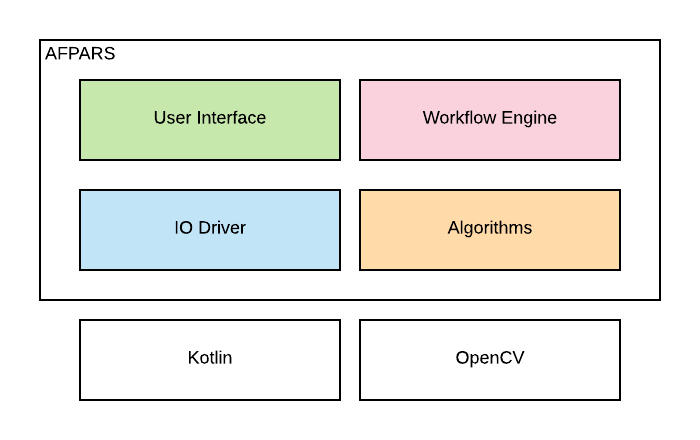
\includegraphics[width=0.8\textwidth]{AFPARS_Architecture}
  \caption{AFPARS software architecture.}
  \label{fig:AFPARS_Architecture}
\end{figure}


To fulfill these requirements, the architecture of the software is split into four parts as shown in figure \ref{fig:AFPARS_Architecture}. The complete application is based on the \acrfull{acro:JVM} on which \gls{gloss:Kotlin} is running. For image processing and recognition the application uses the library \gls{gloss:OpenCV} in version 3.1.

Every part of the architecture has its own area of responsibility and is connected with the other parts through interfaces which have been designed to be as generic as possible to support the most flexibility.

\subsection{Programming Language}

The software is built with the modern language \gls{gloss:Kotlin}, which is a statically typed programming language for the \acrfull{acro:JVM}. It supports special language features like extension methods, optional parameters and functional programming concepts, which all were used in this project and help to make the code more readable and maintainable \citep{kotlin}.

\subsubsection{Extension Methods}
This section shows an example of how the new language is used in the software.

The language feature \textit{Extension Methods} can be used to make the code more readable. It extends an existing object with a new method, however, without the concept of inheritance. The code of the method will be outsourced into a separate file.

\begin{lstlisting}[caption={Erode image without extension methods},label={lst:imageOperations},language=Kotlin]
// threshold image
Imgproc.threshold(image, image, 128.0, 255.0, 
		Imgproc.THRESH_BINARY)

// erode image
val structureSize = 3
val element = Imgproc.getStructuringElement(Imgproc.MORPH_RECT, 
        Size(structureSize.toDouble(), structureSize.toDouble()))
Imgproc.erode(image, image, element)
\end{lstlisting}

It is used in this software to make calls to \gls{gloss:OpenCV} more natural for object oriented developers. For example, instead of using the static Imgproc class (Listing \ref{lst:imageOperations}), it is possible to call a lot of methods on the Mat object itself (Listing \ref{lst:imageOperationsWithExtensions}).

\begin{lstlisting}[caption={Erode image with extension methods},label={lst:imageOperationsWithExtensions},language=Kotlin]
// threshold image
image.threshold(128.0, 255.0, Imgproc.THRESH_BINARY)

// erode image
image.erode(3)
\end{lstlisting}

\subsection{Meta Format}
\label{sub:MetaFormat}
To support the different input and output formats, the architecture uses a meta format for the
floor plan images, called \textit{AFImage}. Different \gls{gloss:Drivers} add the support for multiple file formats. With this architecture it is possible to extend the software with new file formats and work internally with the meta container format.

The meta container \textit{AFImage} contains a map of attributes (Figure \ref{fig:AFImage_CD}), which can be used by algorithms to get information created by other algorithms or to store information into an existing image.

\begin{figure}[H]
  \centering
      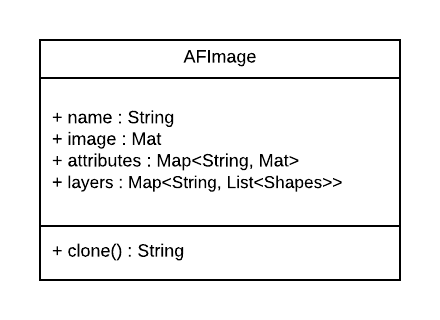
\includegraphics[width=0.6\textwidth]{AFImage_CD}
  \caption{\textit{AFImage} class diagram.}
  \label{fig:AFImage_CD}
\end{figure}

To interact with the user interface there is also a map of layers which contain shapes that are printed onto the image. The software uses this for example for recognised doors or rooms, which are shown as overlay.

By default there is an attribute called \textit{originalimage}, which is a copy of the original image, read by the AFImageReader. This is used in some algorithms to have access to the original, unprocessed picture.

\subsection{Input \& Output}
\label{sub:ImportExport}
The following sections gives a brief overview about the different input and output formats used by the software.

\subsubsection{Raster Graphics}
For importing floor plans into the software the decision was made to only read raster graphics like JPEG or PNG file formats. Raster graphics are flat pixel based images like pictures captured by a photo-camera.

The disadvantage of this restriction is, that raster images do not contain any layers or information about objects of the floor plan. Usually floor plans are stored in a \gls{gloss:DXF} or \gls{gloss:DWG} file format and contain different layers with multiple objects, which could be used to simply detect doors and walls and other steps which are done in the semantic analysis.

\begin{figure}[H]
	\centering
	\subfloat[Layers of 50er EG.]{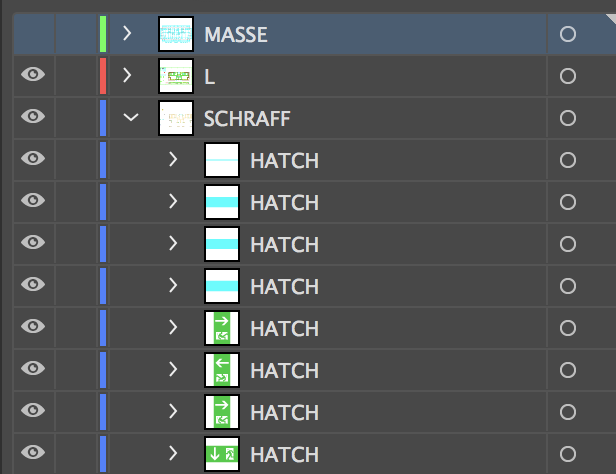
\includegraphics[width=0.3\textwidth]{layers_50er_eg}\label{fig:layers_50_er_eg}}
	\hfill
	\subfloat[Layers of A N1.]{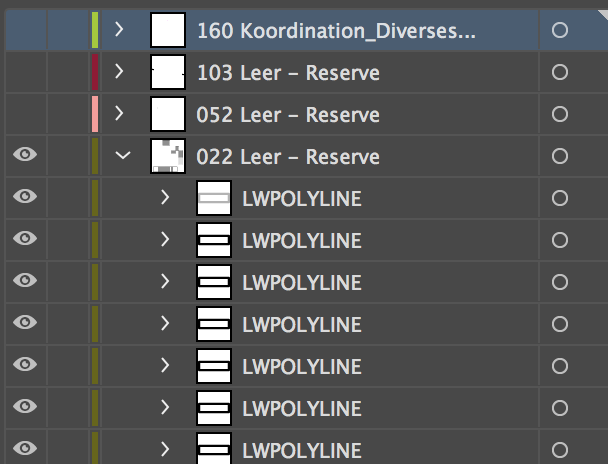
\includegraphics[width=0.3\textwidth]{layers_a_n1}\label{fig:layers_a_n1}}
	\hfill
	\subfloat[Layers of OG.]{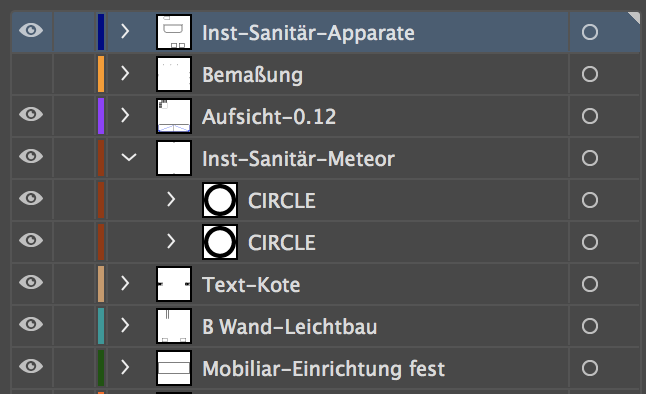
\includegraphics[width=0.3\textwidth]{layers_og}\label{fig:layers_og}}
	\caption{Layers of different DWG floor plans. }
	\label{fig:layer_comparison}
\end{figure}

As figure \ref{fig:layer_comparison} shows, there is no convention or standard for the layer structure of a \gls{gloss:DXF} or \gls{gloss:DWG} file. This problem led to the decision to not work with vector based graphic formats as input and only work with raster images of floor plans.

The advantage of working with raster graphics is that the software is able to use conventional methods for image processing, like pixel based filters.

\subsubsection{DWG / DXF}
As requested by the client, the software should support the import and export of DWG and DXF formats. These file formats are standard in the architectural environment and can be imported and exported by the software AutoCAD, developed by the company Autodesk.

There are several libraries for Java which support reading and writing of DWG and DXF files, but a lot of them are not maintained anymore or cost something. The table \ref{tbl:DWGEvaluationResult} shows the evaluated libraries, including the reason, why they are not suitable for this software (Please consult table \ref{tbl:DWGEvaluationMatrix} in the appendix for an extended comparison).

\begin{table}[H]
\centering
\caption{DWG / DXF evaluation result.}
\label{tbl:DWGEvaluationResult}
\begin{tabular}{@{}lll@{}}
\toprule
Name         & Vendor         & Reason                                               \\ \midrule
YCAD Library & Ed Karlo       & No documentation and very unintuitive.                \\
Teigha       & ODA            & Too expensive and only for conversion.               \\
Kabeja       & -              & Could not read the example document.                 \\
Tika         & Apache         & Only a meta text reader.                             \\
jnetcad      & Johannes Raida & Only a converter.                                    \\
CaffViewer   & DeCaff         & Too expensive but able to read the example document. \\ \bottomrule
\end{tabular}
\end{table}

The only library which could read the test document provided by the client is the CaffViewer. But it is licensed under a closed source license and costs about 1350 Euro.

\subsubsection{Scalable Vector Graphics}
Because DWG and DXF support could not be implemented, rooms and other shapes, which the software recognises, can be exported to \gls{acro:SVG}.

In contrast to the raster image format, the \gls{acro:SVG} file contains commands to draw the image in a later step. This is useful because it enables the resizing of images, without loss of quality and the possibility to select every single element of the image.

With \gls{acro:SVG} it is possible to create an overlay for an existing plan.

\subsubsection{Comma-separated Values}
For exporting the different rooms and their room size, the software contains \gls{acro:CSV} format support. This file format is used to store table data like Microsoft Excel data-sheets.

\subsection{Algorithm}
\label{sub:algorithm}
The architecture of the algorithms follows the single responsibility principle \citep[p.~484]{mclaughlin_pollice_west_2010}. To simply reuse and replace algorithms in a pipeline, every algorithm is responsible for solving just one problem. For example, the morphological transform algorithm is solely responsible for creating a clean image of a given input image and has no other task to do.

\begin{figure}[H]
  \centering
      \includegraphics[width=0.6\textwidth]{IAlgorithm_CD}
  \caption{Algorithm interface class diagram.}
  \label{fig:IAlgorithm_CD}
\end{figure}

An algorithm is context unaware and stateless. It gets an input image and returns an output image which is enhanced by more information or pixel based processed (Figure \ref{fig:IAlgorithm_CD}).

\subsubsection{History}
As seen in figure \ref{fig:IAlgorithm_CD} and figure \ref{fig:parameter_window}, an algorithm is not just able to return one \textit{AFImage}, instead it can return an unlimited count of \textit{AFImages}, which then are displayed in the parameter window. These images are used to show a history of the steps the algorithm performed. This makes it easier to set the right parameter for the given algorithm and helps to debug all steps of an algorithm.

\subsection{Workflow \& Workflow Engine}
To create a pipeline which connects multiple algorithms together, there is the concept of workflows. A workflow is a list of algorithms which have a defined order in which they are executed.

The reason why there is the possibility to define multiple workflows, is because the user can run different combinations of algorithms parallel to one other or to test out multiple versions of pipelines. With workflows it is also simple to implement a flexible system, where the user is able to create new combinations of algorithms on his own.

\begin{figure}[H]
  \centering
      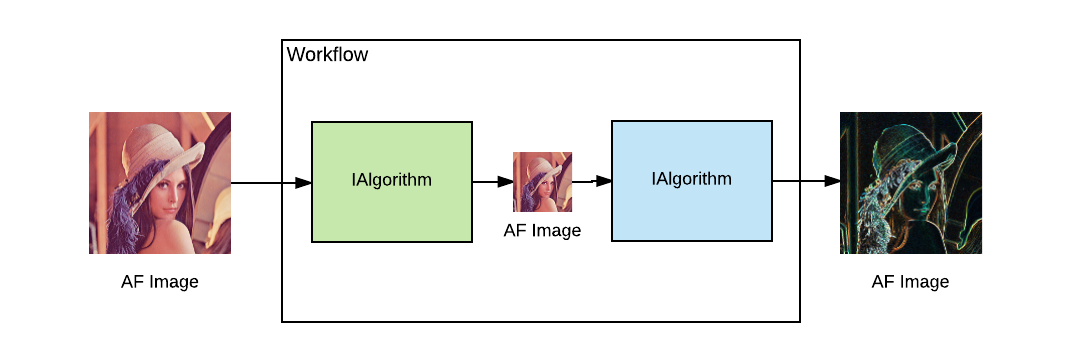
\includegraphics[width=1\textwidth]{workflow}
  \caption{Workflow example with two algorithms.}
  \label{fig:Workflow}
\end{figure}

The execution of a workflow is managed by the workflow engine which takes a workflow and an input image and passes the image through the different algorithms defined in the workflow (Figure \ref{fig:Workflow}).

\begin{figure}[H]
  \centering
      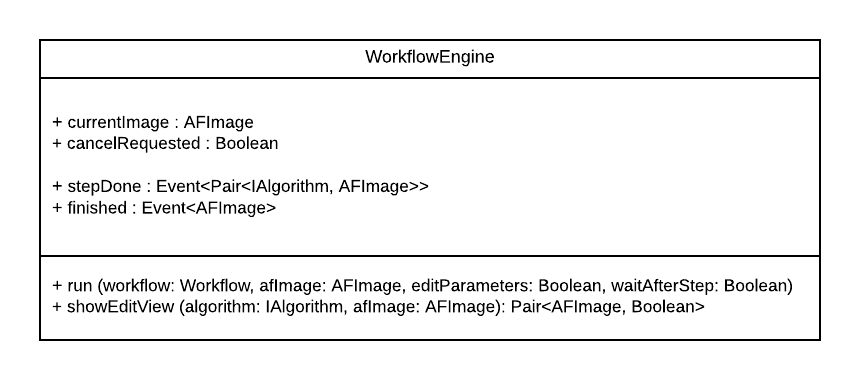
\includegraphics[width=0.8\textwidth]{WorkflowEngine_CD}
  \caption{Workflow engine class diagram.}
  \label{fig:WorkflowEngine_CD}
\end{figure}

The workflow engine runs the workflows in a new thread and communicates with the application through events. It is possible to stop the workflow after each algorithm and make changes to the current \textit{AFImage} of the process. This feature is used to let the user fix recognition errors.

It is also possible to show the parameter window which is described in the following chapter (Figure \ref{sub:parameter_window}).

\subsection{User Interface}
\label{sub:userInterface}

The user interface of the software is designed to be user friendly and very intuitive. It guides the user through the process and offers the tools to fix algorithm errors. The interface itself is very simple and contains only the controls which are absolutely necessarily (Figure \ref{fig:afpars_window}).

\begin{figure}[H]
  \centering
      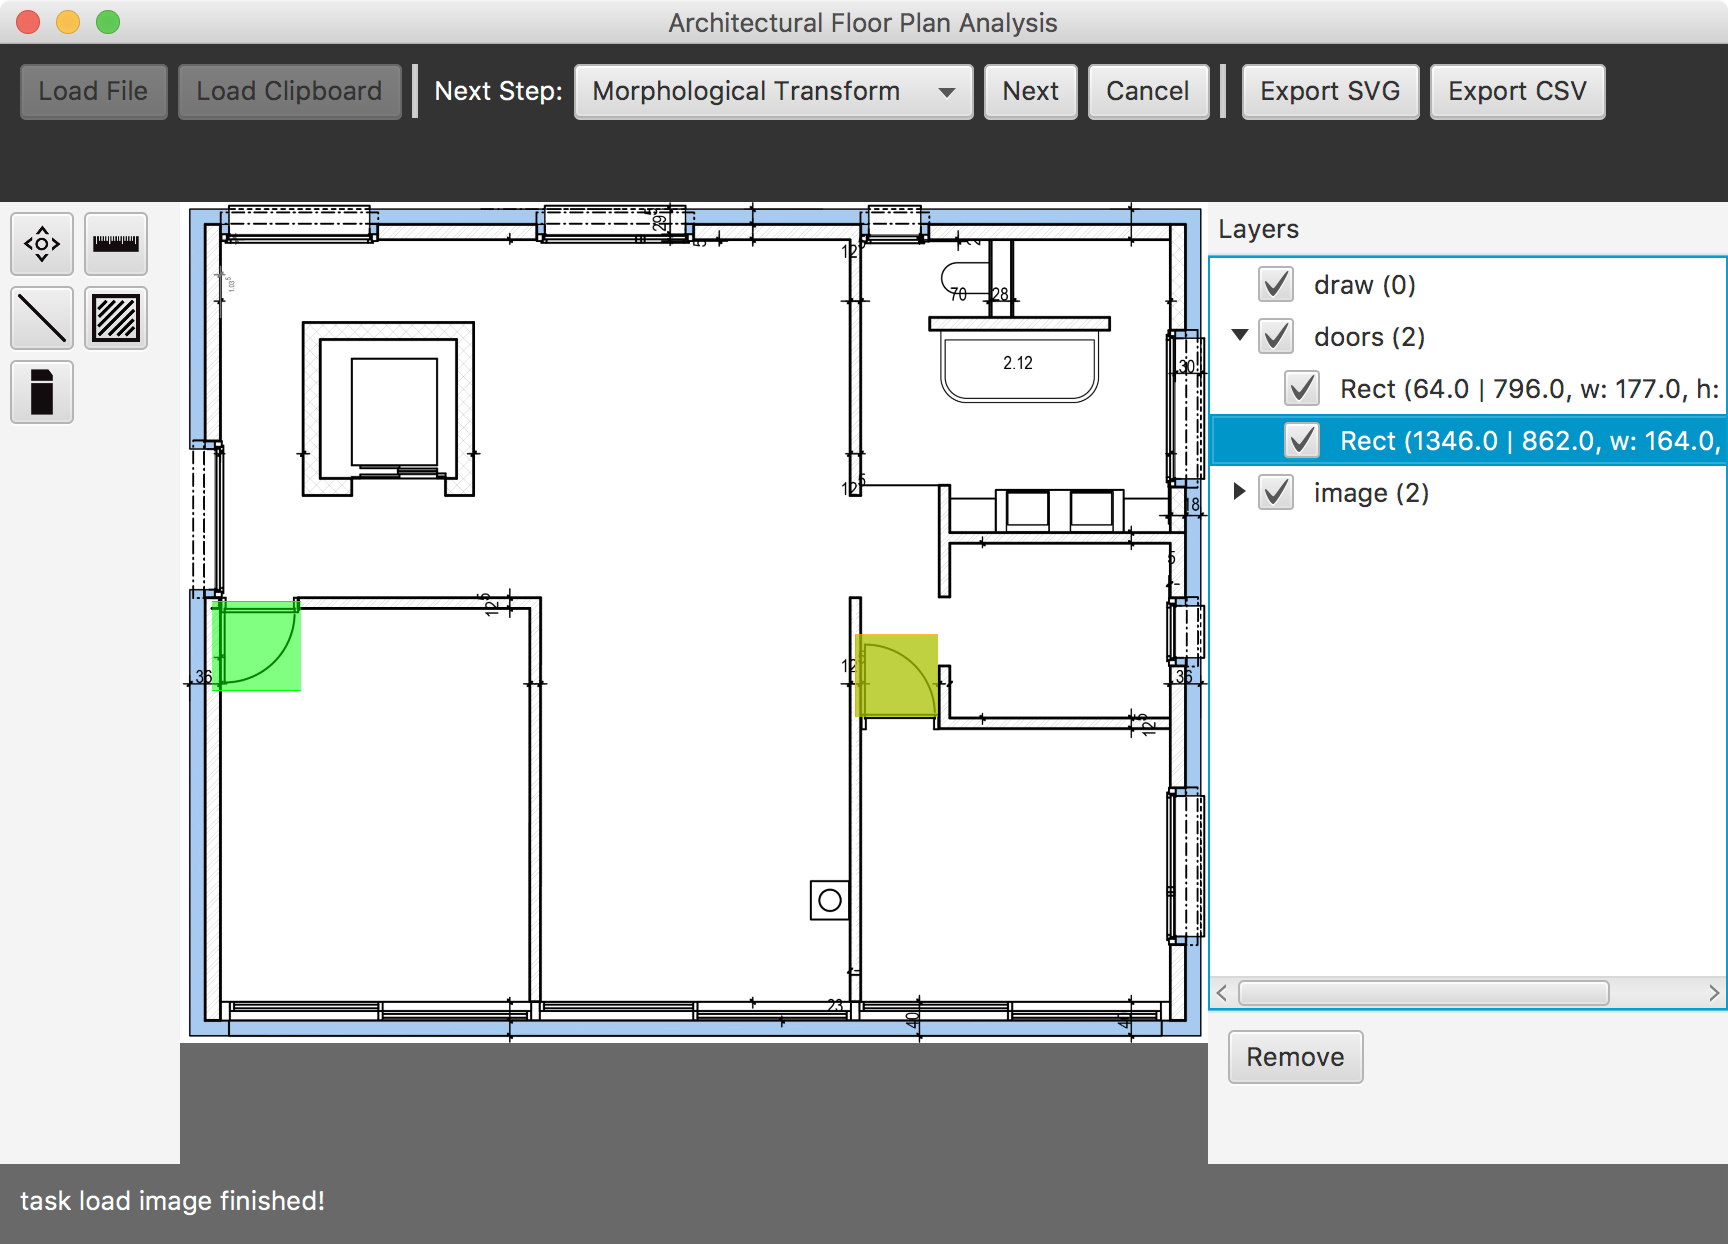
\includegraphics[width=1\textwidth]{afpars_window}
  \caption{Main window of the software.}
  \label{fig:afpars_window}
\end{figure}

\subsubsection{Integration}
During the development process the decision was made to not use an existing application infrastructure like, for example, \gls{gloss:ImageJ}, to host the user interface of this project.

The reason behind this decision is, that the user interface has to fulfil a lot of requirements and should be as intuitive to a normal user as possible. \gls{gloss:ImageJ} and other image processing applications have too many features on board which would not be helpful to guide the user through the process of the application.

\subsubsection{Layout}

The layout of the interface is inspired by popular design softwares like Adobe Illustrator or Autodesks AutoCAD. The different parts of the layout are shown in figure \ref{fig:afpars_window_zones}.

At the top is the navigation section which guides the user through the process of the application. The navigation buttons are arranged in a sequential manner to reflect the application workflow. First of all, the user has to load the image from a file or the clipboard. After that he is able to start the workflow and run through the different steps.

After finishing the workflow, the user has the possibility to export the different layers or a \gls{acro:CSV} file with all the detected rooms and room sizes.

The canvas section is located at the center of the window and acts as the applications drawing pane. It always shows the current image of the process and lets the user correct and inspect the algorithm output.

To edit the current image, there are tools on the left side of the window. Those controls change the current tool used to manipulate the image.


\begin{figure}[H]
  \centering
      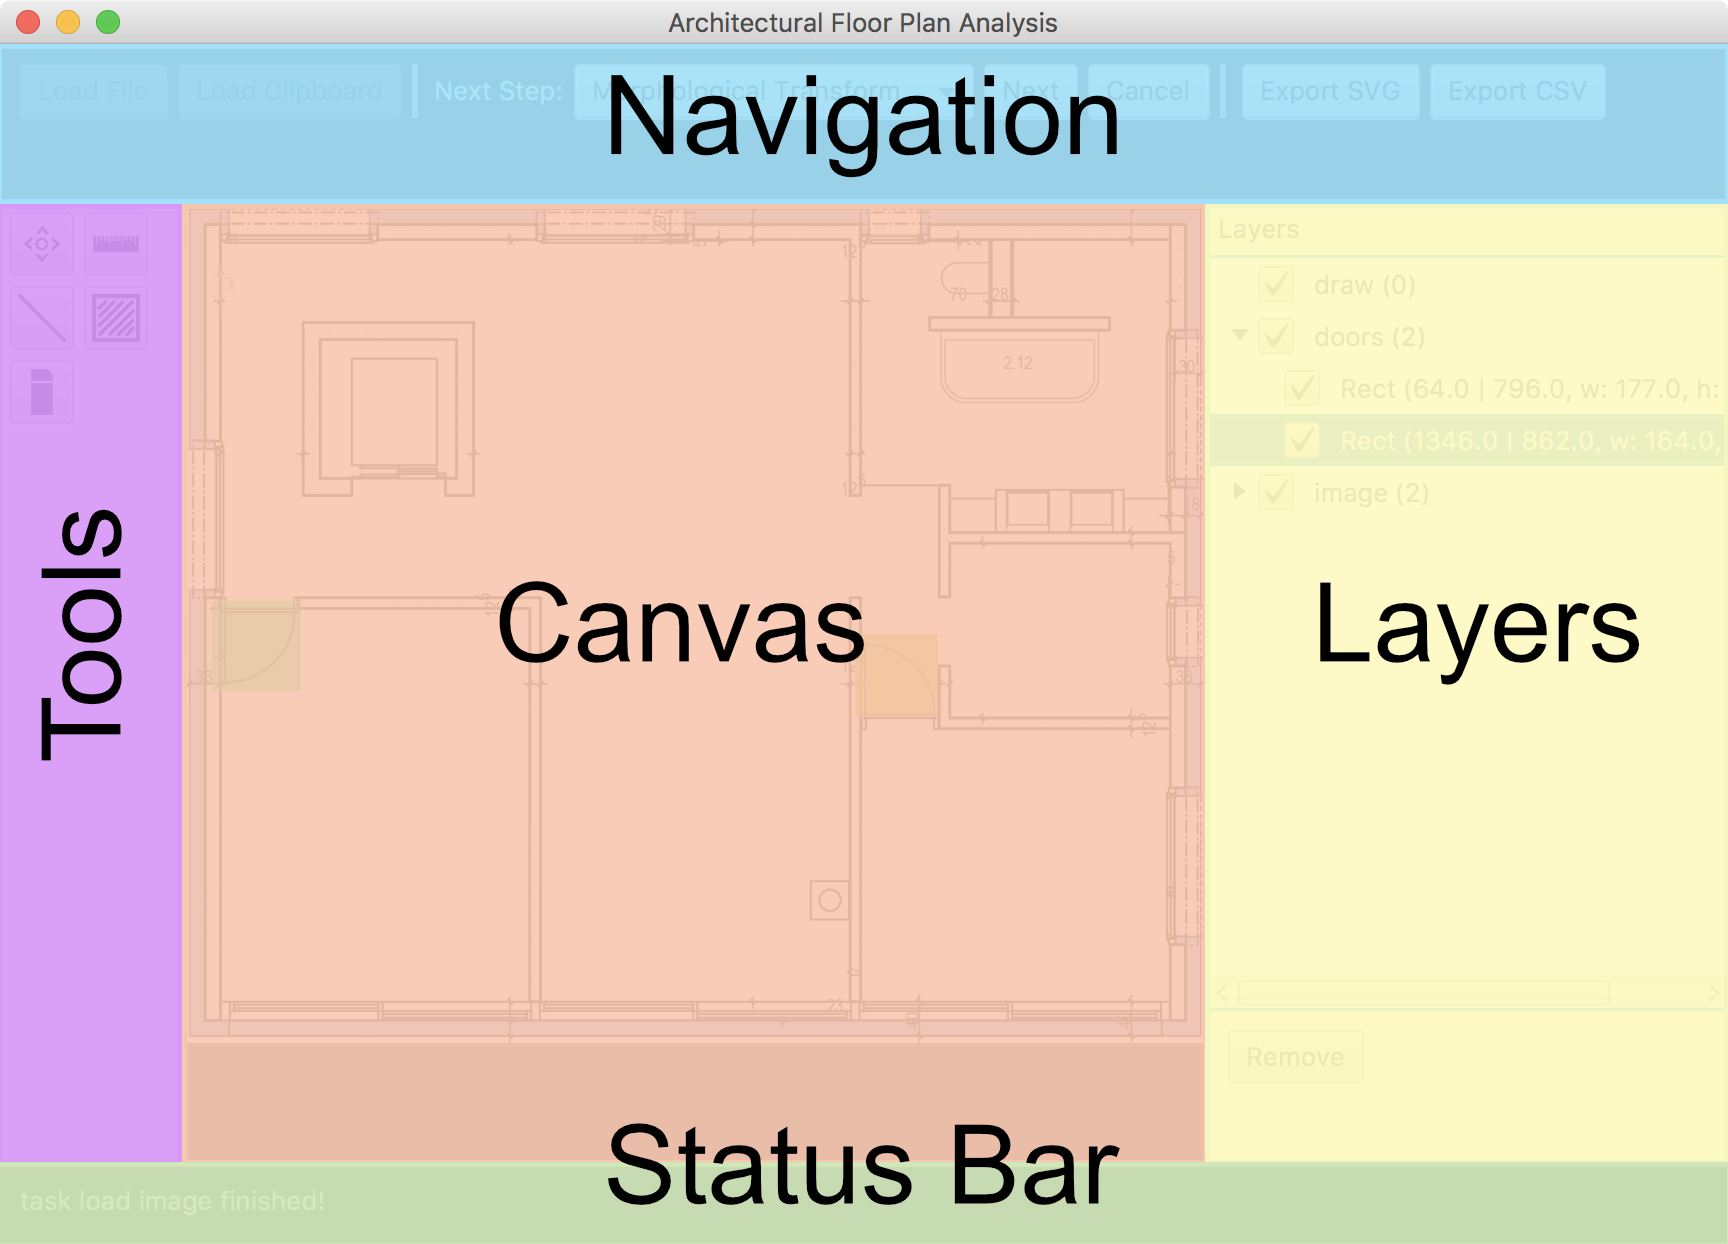
\includegraphics[width=1\textwidth]{afpars_window_zones}
  \caption{Main window with zones.}
  \label{fig:afpars_window_zones}
\end{figure}

On the right side of the application window, is the layer section. The layer section shows the different layers which are printed onto the canvas. Each layer contains shapes which can be toggled as visible or not. There is always a draw layer which contains all the drawings done by the tools on the right side. It is also possible mark these drawings and to delete them if needed.

Only drawn shapes and detected rooms can be deleted through the user interface. Every other layer is locked and can only be disabled.

At the base is the status bar which shows the status of the different task the user interface is performing.


\subsubsection{Parameter Window} \label{sub:parameter_window}
Because a lot of the algorithms need parameters to be set manually, there is the possibility to flag these parameters with an attribute in the code and the software is then able to automatically detect them and show an input field in the user interface. With this input field the user is able to set the parameter or use the default values (Figure \ref{fig:parameter_window}).


\begin{figure}[H]
  \centering
      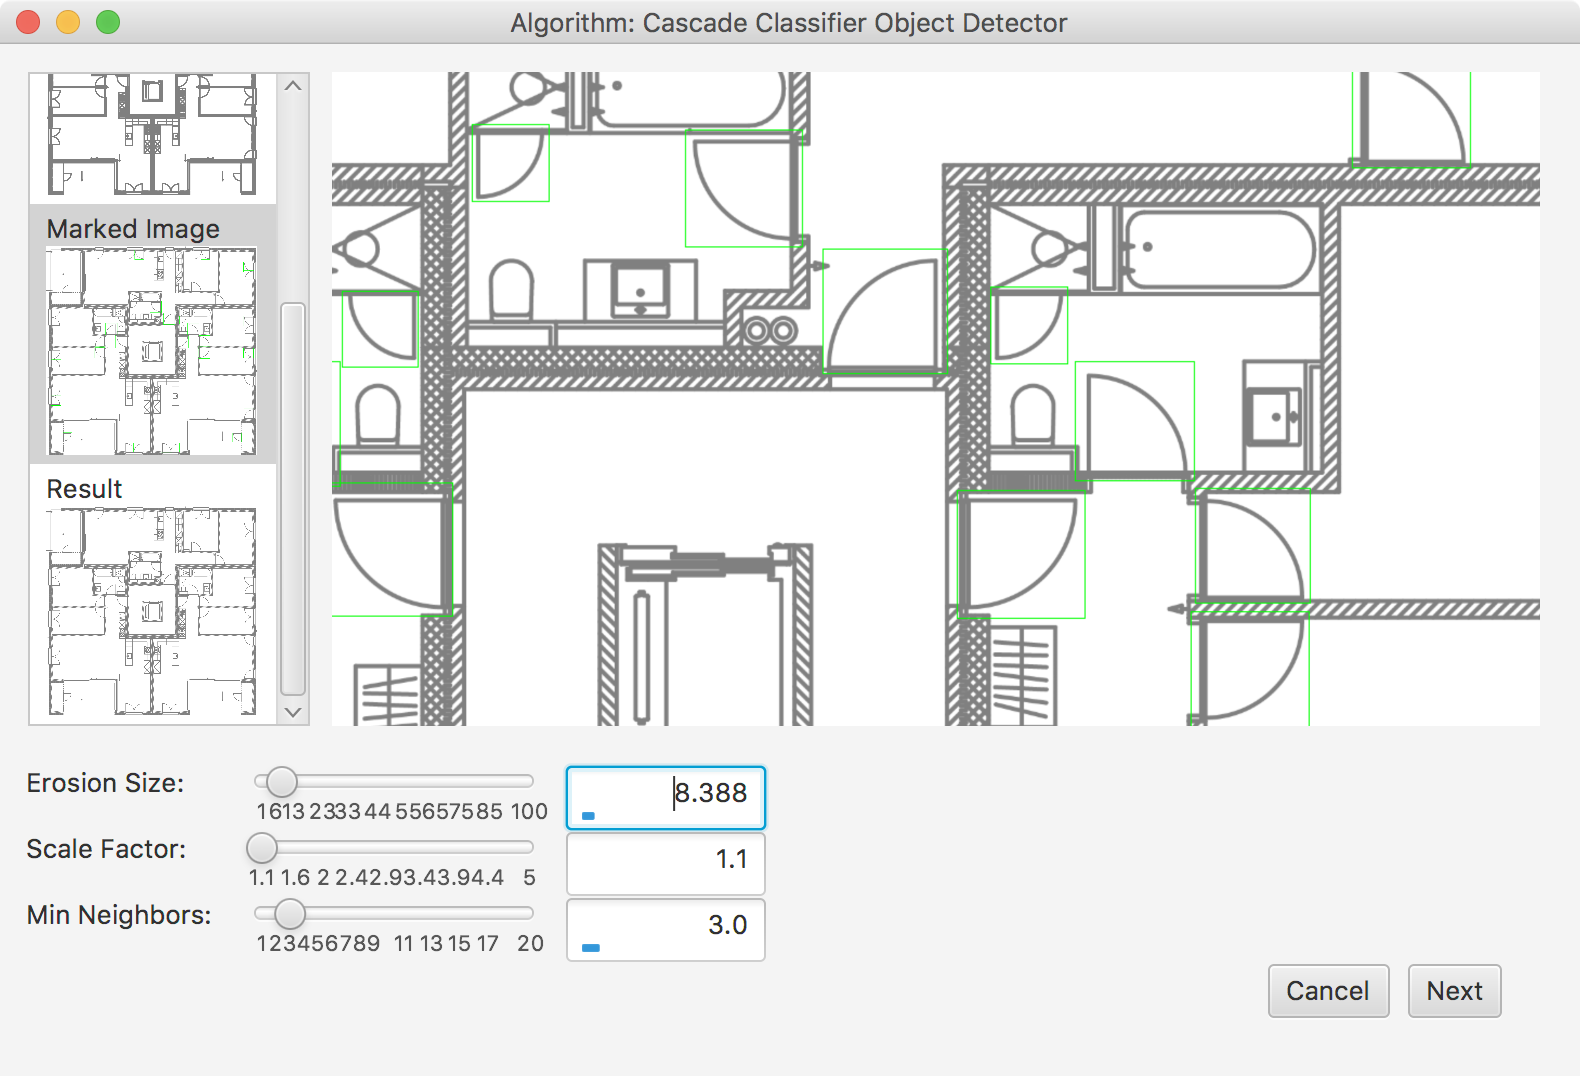
\includegraphics[width=1\textwidth]{parameter_window}
  \caption{Algorithm parameter window.}
  \label{fig:parameter_window}
\end{figure}

This parameter window is shown by the application when an algorithm is started. It runs the algorithm once and then shows its output of it in the preview window. Each change in the parameters makes the algorithm run again. With this behaviour the user always gets an instant visual feedback of the changes he has made.
\section{Implementation}
\label{sub:Implemenation}
The following sections describe, how the implementation of the automatic room recognition was achieved. Basically it is split into three parts, later called workflows. Each workflow is a combination of algorithms, which solves a different problem.

Every section will describe why and how the algorithm is implemented and what the results of the implementation was.

\subsection{Workflow 1}
\label{sub:workflow1}
This section describes the first combination of algorithms that was implemented to try and achieve room detection. It is based on research of the paper by Ahmed, Liwicki, Weber and Dengel \citep{mace_valveny_loctea_tabbone_2010} to find the walls in an image with a Hough transformation. To then detect the rooms, the idea was to detect them with a watershed algorithm. This algorithm is used by several projects on the internet, on the context of room segmentation. The general idea, how this algorithm is supposed to work and what problems were found, are described in this section.

\begin{figure}[H]
	\centering
	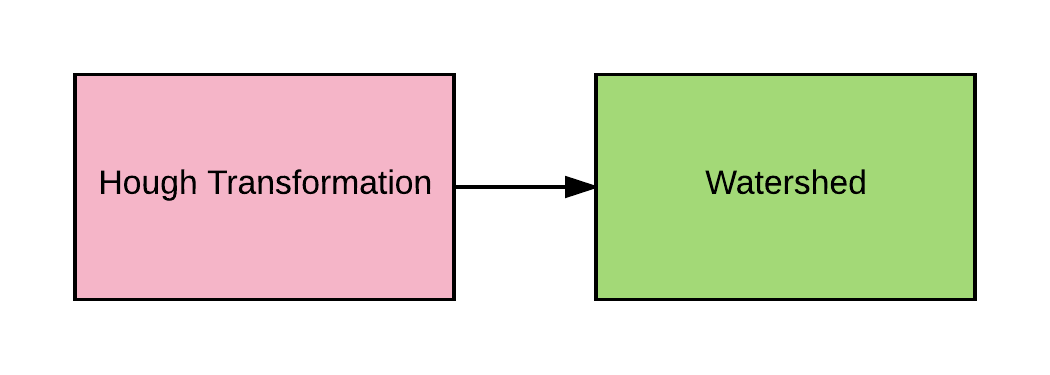
\includegraphics[width=0.6\textwidth]{Workflow1Flowchart}
	\caption{Workflow 1 flowchart.}
	\label{fig:Workflow1Flowchart}
\end{figure}

\subsubsection{Hough transformation}
This implementation is based on the fact that the Hough transformation will find long lines on an image. These lines will usually be the walls. Cleaned up images of architectural floor plans were used to start off. This was done to remove noise on plans so the walls could be extracted easily.

As described in section~\ref{subsubsec:Hough transformation}, the Hough transformation finds straight lines on an image. Long straight lines on a floor plan are usually the walls, therefore the Hough transformation is supposed to detect them on the plan. As a precondition for the Hough algorithm, a binary image is needed. To create this binary image, we use the Canny Edge detection algorithm by OpenCV. Wherever it detects an edge, the pixels will be white, all other pixels will be black. There will be two edges for each wall, one where the background changes to the wall and the other, where the wall ends and the background starts again. To then detect the lines, the Hough transformation by OpenCv, called HoughLines, was used first. It finds all the suspected lines and returns it in an array represented with the $(r,\theta)$ orientation representation. The problem with this implementation was, that this just represents the orientation and location of the line but not its size.
As a replacement HoughLinesP was used. It does the exact same, but additionally calculates where those lines actually are. The resulting array returns the actual starting and ending position of the lines. 

There were several problems with that algorithm. The algorithm separated a wall line into a lot of small lines. To retrieve the actual wall there would have to be additional computation that connects those several small parts into one big line. As an addition, due to no preprocessing, what was left as a wall, were the actual outlines of the original walls. Therefore, any wall was represented by two parallel lines. This would have led to additional effort. Before any of those efforts were made, a different algorithm was found that showed more promising results. Therefore the optimization of this algorithm was not pursued further.

  
\subsubsection{Watershed}
The idea to find the different rooms within the floor plan, was to run the watershed algorithm on the image (Section~\ref{subsub:watershed}). It is a flood filling algorithm that starts at given starting points and extends its area, until it meets a wall or a different flood from an other starting point. A further explanation will be done in section~\ref{subsubsub:watershed}, as it was actually implemented and used in our second workflow.

\pagebreak

\subsection{Workflow 2}
\label{sub:workflow2}
This section describes the second workflow and what algorithms it is composed of. It is a mix of the work of Sébastien Macé and Peter Dawkins and Hervé Locteau and Salvatore Tabbone~\citep{mace_valveny_loctea_tabbone_2010} and the experiences we made with the first workflow~\ref{sub:workflow1}. What it does, is it removes any noise on the floor plan first with morphological operations, like erosion and dilation. This is followed up with a room detection algorithm that, in the end, uses the watershed algorithm to determine the rooms. In contrast to the first workflow, where the preprocessing for the watershed was not done sufficiently, this algorithm improved that. After optimizing this workflow, it was the first workflow that showed actual potential and was able to detect the rooms and therefore solve the given problem.


\begin{figure}[H]
	\centering
	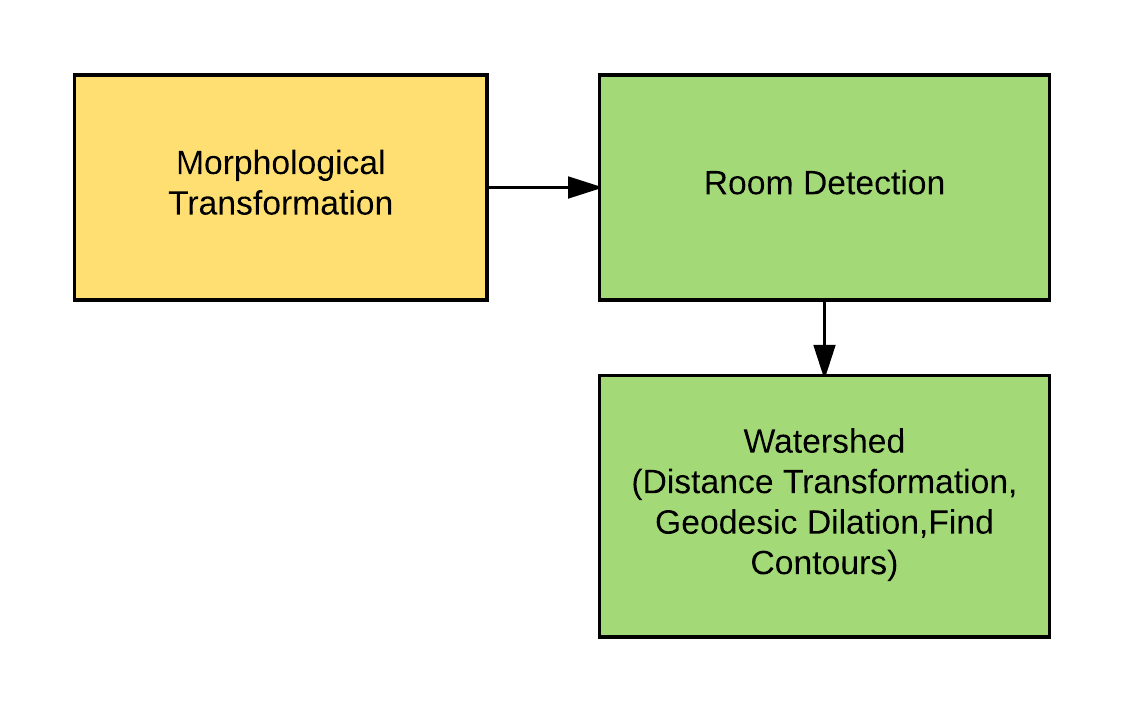
\includegraphics[width=0.6\textwidth]{Workflow2Flowchart}
	\caption{Workflow 2 flowchart.}
	\label{fig:Workflow2Flowchart}
\end{figure}

\subsubsection{Noise removal}
All of the following topics in this section are used to remove or add specific information from our image. The idea is to standardize all incoming floor plans regardless of what "noise" is around in the basic floor plan. Noise is anything that is of no importance to all the following algorithms. This contains elements such as "personal-property" (cars, pianos, etc.) as well as text or any lines to show dimensions on the plan. The idea would be that most of this noise is erased by the user in advance. But it is practically impossible to remove all the noise beforehand, due to it being so time intensive. It would ruin all the benefits of the algorithm, which uses less time than doing everything by hand.

\paragraph{Morphological transformation}
\label{sub:MorphologicalTransformation}

The basic principle to remove noise is erosion and dilation. How the algorithm is processed is explained in section~\ref{subsubsec:Erosion and Dilation}.
The purpose of both of those algorithms in this project is to remove any information on the starting picture, to get a picture containing only the walls. This works due to the fact that usually the walls are the thickest lines on the floor plan. It is a simple heuristic to extract the walls and is according to the method other papers use (see \citep{ahmed_liwicki_weber_dengel_2012}).

This project always uses a combination of erosion and dilation to retain the original place of all the walls. The size of the rooms would differ from the original size if we did not do the same dilation after an erosion and vice versa. This would render all the results useless, since a basic requirement is to find the actual room polygon. There are two ways to use noise removal as a combination of erosion and dilation. 

\begin{description}[style=nextline]
	\item[Erosion first] This removes thin lines from the image. Those are non walls and therefore of no importance to the output image. The dilation brings the remaining lines back to its original size.
	\item[Dilation first] This extends all lines and combines any lines that are close to each other. The erosion following then creates one line out of the bunch. This is used to combine walls that are created out of several thin lines into one thick line.
\end{description}

Both of those combinations are used in the morphological transformation class. First used is the "dilation first" transform to combine the walls out of several lines into one. This results in all the walls being one thick line instead of a multitude of small lines. This guarantees that all walls are thick lines and won't get erased with the "erosion first" transform. This is now followed with the "erosion first" transform to erase all the other lines besides the walls. 

\begin{figure}[H]
	\centering
	\subfloat[Original image.]{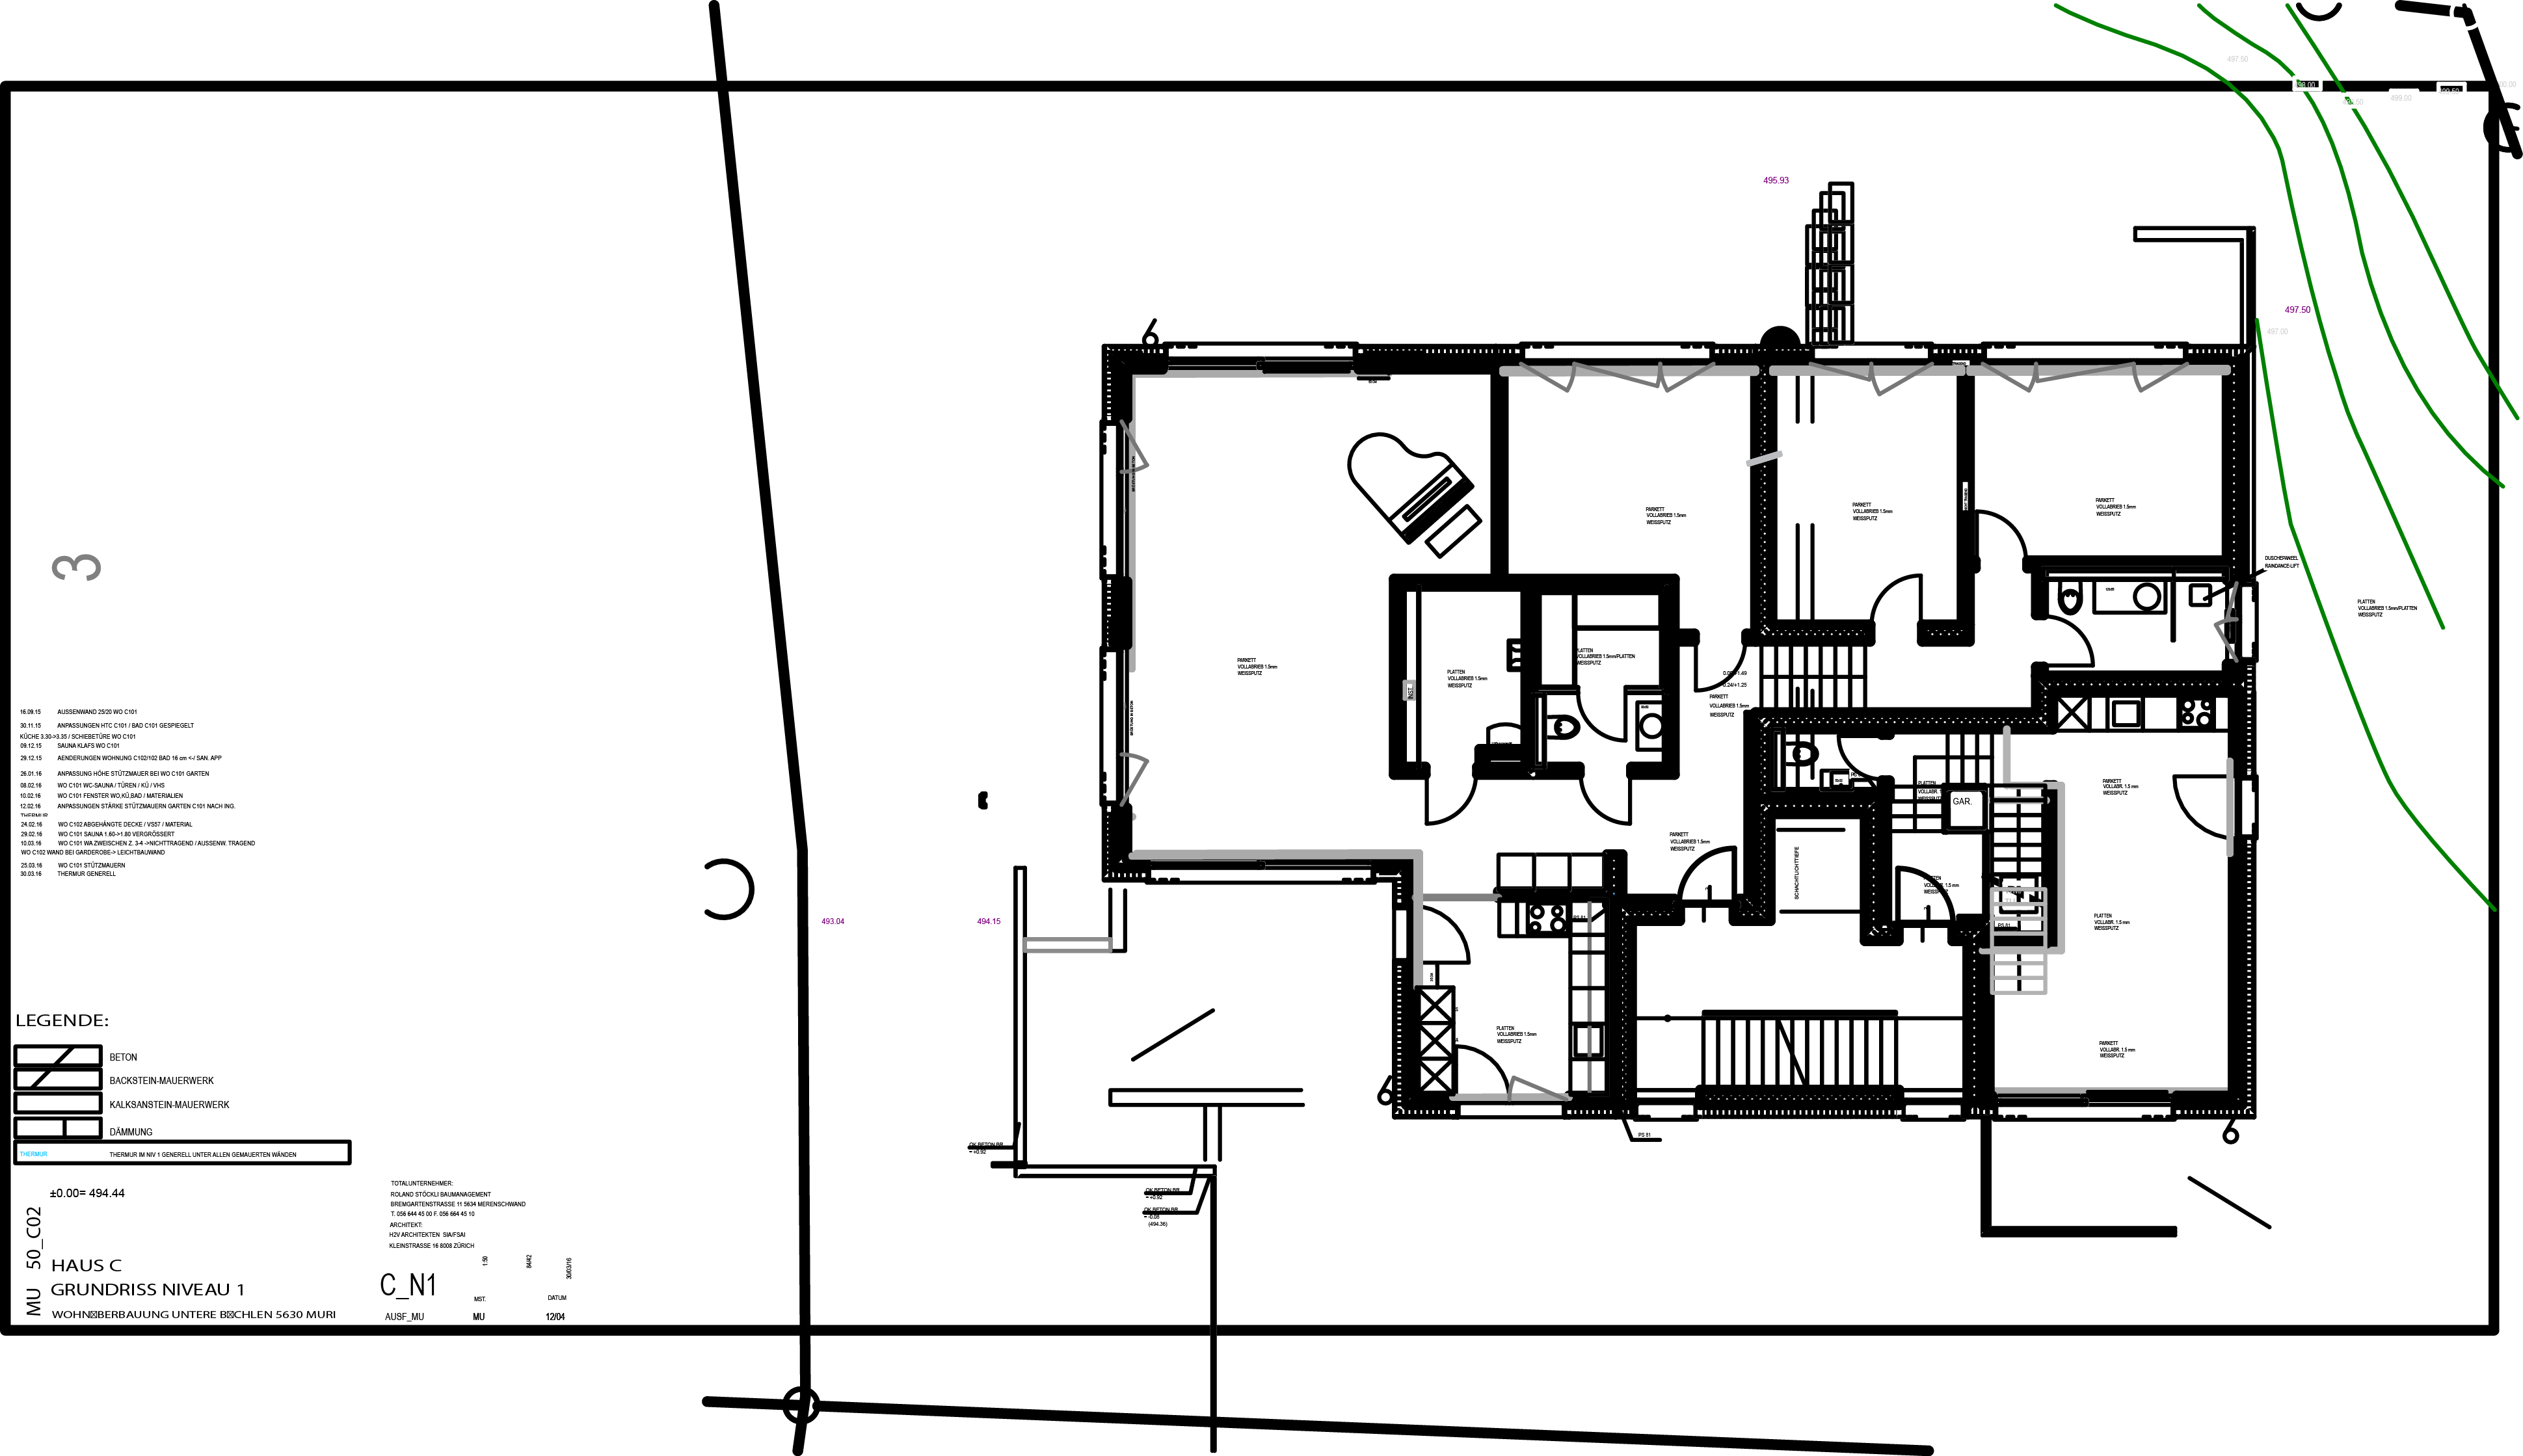
\includegraphics[width=0.5\textwidth]{A_N1.png}\label{fig:A_N1}}
	\hfill
	\subfloat[Image after noise removal.]{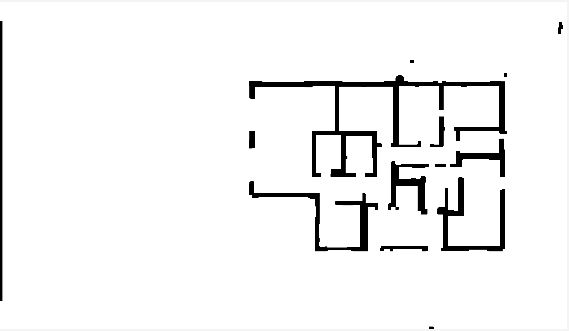
\includegraphics[width=0.4\textwidth]{morphtransuncleaned.jpg}\label{fig:A_N1_Morph}}
	\caption{Before and after of an uncleaned floor plan with noise removal. }
\end{figure}

\begin{figure}[H]
	\centering
	\subfloat[Original image.]{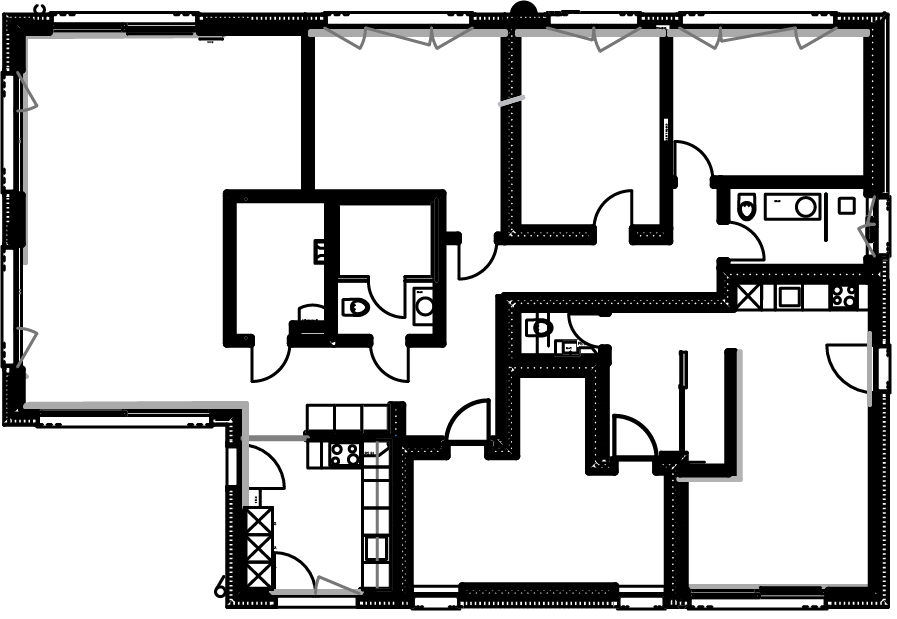
\includegraphics[width=0.5\textwidth]{A_N1_cleaned.png}\label{fig:A_N1_cleaned}}
	\hfill
	\subfloat[Image after noise removal.]{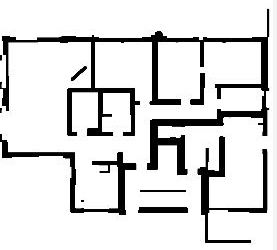
\includegraphics[width=0.4\textwidth]{morphtranscleaned.jpg}\label{fig:A_N1_cleaned_Morph}}
	\caption{Before and after of a cleaned floor plan with noise removal.}
\end{figure}

The figure~\ref{fig:A_N1} is one of the uncleaned testing images before any noise removal. It was cleaned up with an erosion/dilation size of 8. Figure~\ref{fig:A_N1_Morph} is the result of the noise removal. It is easily visible that most of what's left are walls. Due to the thin lines of the windows they get removed in the process. Those will be added later though, as they are an important part of the wall to surround the rooms.

The same was done to the cleaned up image. As a result of different image sizes, the noise removal was actually worse with the same parameters. This shows that each different image has very specific parameters for an optimal noise removal.

As this is not perfect due to the variety of possible objects on a plan, there is the option to delete either before or after with our built in editor. This is so that we can manually improve the quality of the outcome of noise removal.

As a result of the noise removal, we get an image with very basic information about where the walls are. This will be very important for our next step and other steps to come.


\subsubsection{Room detection}
To implement the room detection, the preprocessing had to be improved compared to the first workflow. What was needed is a proper creation of the foreground and background image. The foreground image contains all the centers of the room. Each center receiving its own color value to differentiate them from each other. The background image contains all the walls. Those are then combined into a single image and handed over to the watershed algorithm that then finds the rooms. The center of the rooms are found with a combination of a distance transformation~\ref{sub:DistanceTransformation}, a geodesic dilation~\ref{sub:GeodesicDilation} and a contour finding~\ref{sub:FindContours}. All of those are described in the following paragraphs.

\paragraph{Distance transformation}
\label{sub:DistanceTransformation}
The distance transformation is used to find the centers of the rooms as explained in section~\ref{subsubsec:Distance transformation}. As its base it needs a cleaned up image of all the walls. It is a result of the noise removal we discussed in the previous section. To find the actual area of the of the room there is further processing with a geodesic dilation (Section~\ref{subsubsec:GeodesicDilation}) needed.

The distance transformation gives us an image that represents the distance from the walls (lines in black) as a gradient of grey values going from dark (close to the wall) to bright (farther away). This means that there will be a center in each room that is very bright and has color values close to white.

\begin{figure}[H]
	\centering
	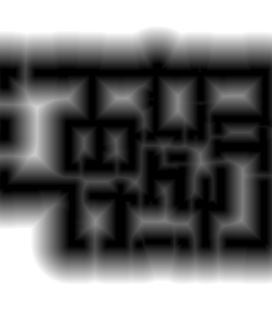
\includegraphics[width=0.6\textwidth]{dist_transform.jpg}
	\caption{Example distance transformation of a architectural floor plan.}
	\label{fig:dist_transform}
\end{figure}

To find the centers, there had to be an additional method that provides us with a specific information where these center areas are.

\paragraph{Geodesic dilation}
\label{sub:GeodesicDilation}
The algorithm to locate the centers after having done the distance transformation is the geodesic dilation~\ref{subsubsec:GeodesicDilation}. The purpose of this algorithm is to find the brightest points in an image and create a marker image. This marker image is a binary image that has all the bright points represented with white color and all other with black color. Based upon the assumption that the distance transformation marked points brighter the further away they are from walls, all room centers consist of bright pixels. Therefore the marker image contains all the room centers. Additionally though, since the plan usually has open space outside the bounding wall, it finds room centers outside of the house as well. The idea was that to close the outside walls and then delete all rooms that are connected to the border of the picture. There is an implementation of this algorithm in workflow 3~\ref{sub:WallClosing}. An implementation of how we tried to avoid this problem is described in the next paragraph about finding contours.

\begin{figure}[H]
	\centering
	
\includegraphics[width=0.6\textwidth]{MarkersGeodesicDilation}
	\caption{This image shows the markers (black areas) for the geodesic dilation of the floor plan AN1.}
	\label{fig:geodesicDilation}
\end{figure}

\paragraph{Find contours}
\label{sub:FindContours}
The find contours algorithm was used to find the centers found in the marker image and give each of those their own color value. This was done so the watershed algorithm automatically creates a border between rooms as soon as the different flooding zones from the algorithm meet each other. This process is further described in the next paragraph. What the find contours algorithm does on the marker image is, that it finds all the borders of the defined centers. With the implementation of findContours in OpenCv you can specify to also fill the found borders with a specified color value. Therefore, each marker found got a new color value. As it is a grayscale image, a base value of 200 was defined and for each new room found we increased that color for that room by one. This gives the option to detect up to around 50 rooms.

\begin{figure}[H]
	\centering
	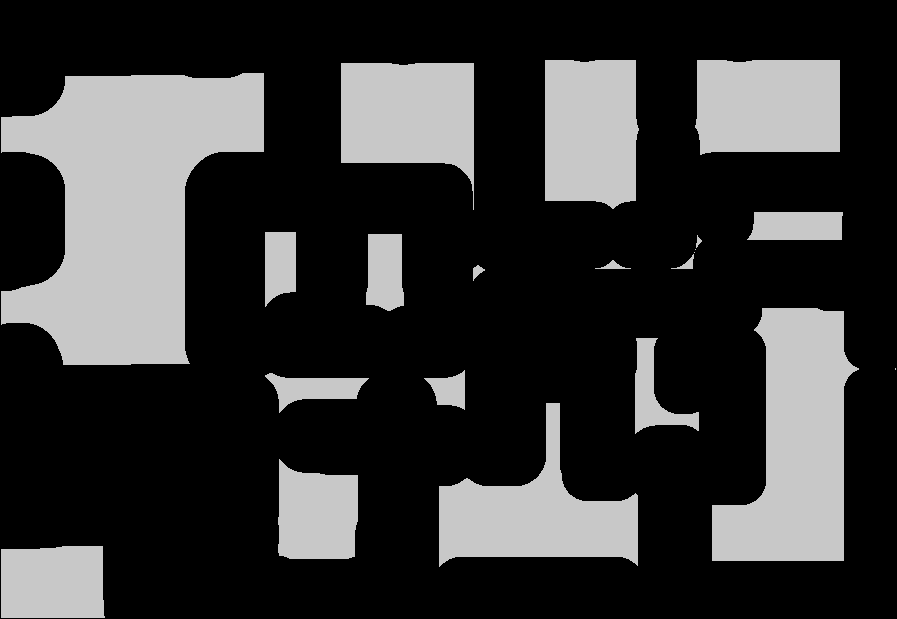
\includegraphics[width=0.6\textwidth]{findContourForeground}
	\caption{This image shows the different marker centers colored in pixel values around 200 and higher on the plan AN1.}
	\label{fig:findContour}
\end{figure}

An additional idea that was tried was to ignore rooms found that had any connection to the border of the image. The findContours algorithm finds a hierarchy on what contour contains other contours. We therefore tried to use the heuristic that the out-most contour that contains all other contours is the contour that contains all "room-centers" that are outside of the house. Therefore this contour could be ignored. As you can see on the image \ref{fig:geodesicDilation}, this heuristic does not work very well as there are too many conditions that can make it fail. One problem was that windows weren't closed and actual room centers existed that connected to the wall itself and therefore were not an inner contour. Additionally, there are sometimes inner contours that are not part of the house itself. As a result of those experiments we came up with a solution that is described in workflow three as wall closing~\ref{sub:WallClosing}.

 
\paragraph{Watershed}
\label{subsubsub:watershed}

The watershed is the core of our room search algorithm. Its purpose is to fill  the unknown areas that are provided in a foreground/background image from previous images. It needs extremely good preprocessing. If it has any previous errors, the resulting rooms will not make sense.

We use the watershed and its ability to find connected rooms with a simple method. It is a simple algorithm that has low computational cost. This and the fact that it was already implemented in openCV, made us use this algorithm.

The algorithm uses a simple image of all the walls as an image to compare to the foreground/background image. This image has been modified with the door recognition algorithm to close all doors within that picture. This is important so rooms are separated when running the watershed algorithm. Additionally, we tried to do a window recognition to close the outside walls. As explained in section \ref{sub:WallClosing}, this did not work out as planned. What we instead used is explained in the second part of section \ref{sub:WallClosing}. With this method we are able to separate all rooms within a building that has no windows on the inside. Any building that has a courtyard will fail with this method. Our goal was to find a solution that can also deal with this. But due to limited time and no reasonable alternative, we chose to go with that.

The background/foreground image is split up in three different zones. The zone with pixel color values of 0 represent the part of the image that are unknown. All pixels with color value 128 represent the walls. As for the rooms, we chose to mark all center with value 200. The image used for comparison has the same areas with walls as the BG-image. This means that the area for the wall will not expand with the watershed. The only exception is the area where doors or windows were closed. This is based on the assumption that the wall has the same pixel color and the inside of the room has a vastly brighter color.
The bright centers of the room inside the BG-image will expand into the unknown areas close to the walls and fill up the rooms. This will result in an image with several enclosed rooms all having the same pixel color. This will be processed with a modified connected component algorithm to find all the edges or the room.

We ran into several problems during the implementation of this algorithm. The most common problem is that not all doors were found. Furthermore, not all rooms have doors to separate them. There are also rooms that are separated with just an open space. There are also objects like cabinets that were drawn with thick lines and were identified as a part of the room. This is easily recognizable as a human but can not be differentiated with the algorithms used.

As a solution to the fact that not all the doors are found, there is the option to close doors by hand with the editor. This is the simplest solution that always guarantees success. We also tried to improve door detection with better samples and bigger sample size. This can be found in the section \ref{sec:ResultsCascade}.
To erase object from the image we initially planned to do an object detection. There was time to do some additional object detection other than just door and window. The cascade files can be found in the code. But there are too many different objects only within those few plans to catch them all. To implement object detection for further objects and erase those objects is a next step for this project. For now the user has to erase all object that do not get caught by noise removal by hand.

\pagebreak
\subsection{Workflow 3}
\label{sub:workflow3}
With all the gained experience in workflow one (Section~\ref{sub:workflow1}) and workflow two (Section~\ref{sub:workflow2}), we started to implement workflow three. This workflow improves the room detection with the use of object detection, to fill gaps caused by the morphological transformation (Section~\ref{sub:MorphologicalTransformation}).

\begin{figure}[H]
	\centering
	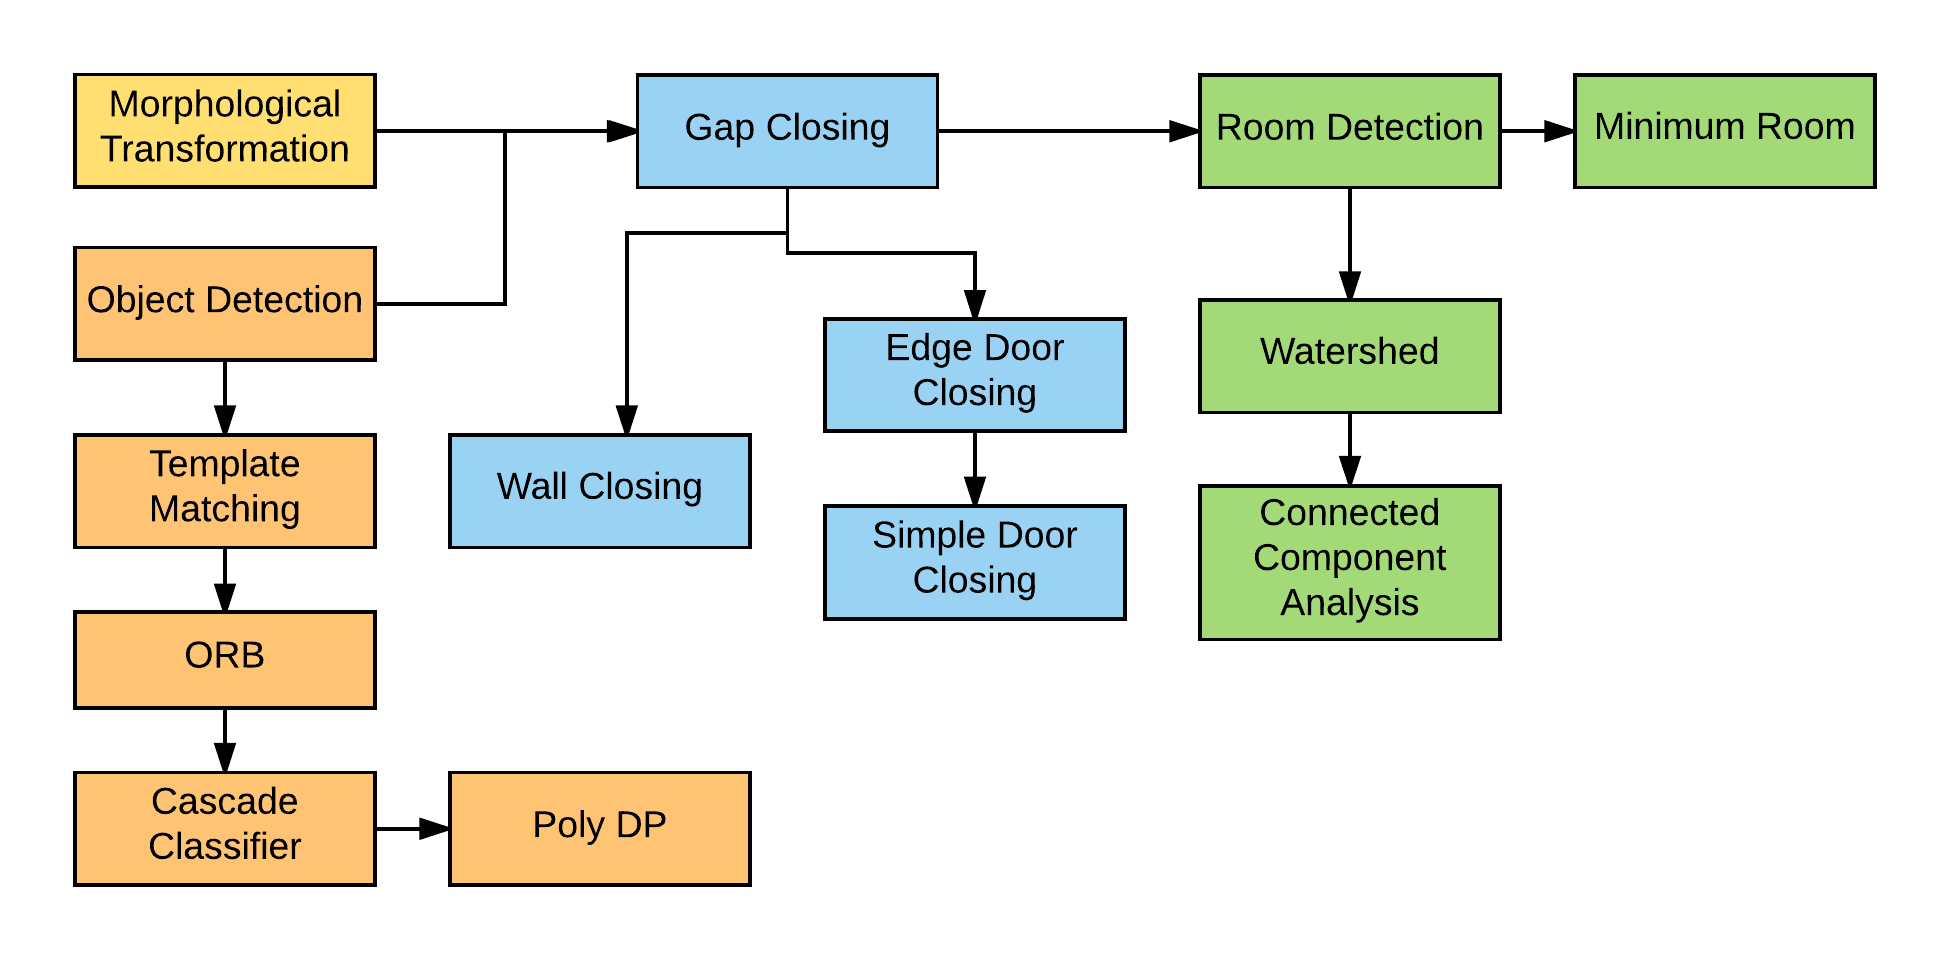
\includegraphics[width=1.0\textwidth]{Workflow3Flowchart}
	\caption{Workflow 3 flowchart.}
	\label{fig:Workflow3Flowchart}
\end{figure}

As shown on figure~\ref{fig:Workflow3Flowchart}, the morphological transformation and object detection step can be run in parallel. Because the user interface needs the assistance of the user, we decided to first run the object detection and then run the morphological transformation.

\subsubsection{Noise removal}
\label{sub:NoiseRemoval}
Noise removal has not been changed from the previous workflow. Morphological transformation is still used in this workflow, to detect the inner and outer walls of the building and to remove unwanted noise from the image like furniture or architectural markings.

For more information about the noise removal, have a look at section~\ref{sub:MorphologicalTransformation}.

\subsubsection{Object detection}
\label{sub:ObjectDetection}
One of the major problems of workflow two (Section~\ref{sub:workflow2}) is, that the morphological transformation erases too many elements from the floor plan. The doors and windows are also removed, but they are needed to separate the individual rooms.

Object detection was contemplated from the beginning of the project, to detect furnishings and other parts of a room, which define the room zones (Section~\ref{sub:RoomZones}). So the idea was to use it to detect doors and windows, and close the gaps between the walls. This would solve the problem of workflow two.

The basic problem was to find an algorithm that can detect objects that vary in their details, regardless of their rotation and size. This is important due to the fact that there is no standard for objects in architectural floor plans that are used by a wide audience of architects. The decision to go with a machine learning approach and not an algorithm that works with heuristics, is because we wanted to be able to process a broad variety of floor plans. Regardless whether they show a small house with just basic features, or a big plan with a lot of details and special objects.

In the following sections, we will take a look at different object detection approaches and how well they performed in detecting doors. The performance for each algorithm will be measured with the F1 score (Section~\ref{sub:F1Score}).

\begin{table}[H]
\centering
\caption{Floor plans with total count of rooms and doors.}
\label{tbl:FloorPlanData}
\begin{tabular}{@{}lll@{}}
\toprule
Name          & Rooms & Doors \\ \midrule
50er\_eg      & 21    & 26    \\
A\_N1         & 9     & 13    \\
A\_1OG        & 50    & 75    \\
Grundriss\_OG & 4     & 2     \\
H\_OG01       & 12    & 19    \\ \bottomrule
\end{tabular}
\end{table}

Table~\ref{tbl:FloorPlanData} shows each test floor plan, with its number of rooms and doors. The data has been raised by hand and does not include doors, windows or closets. This data will be used to calculate the metrics of each object detection algorithm.

To test the algorithms, we decided to just use three of the five experiment images (\textit{50er\_eg}, \textit{A\_N1}, \textit{A\_1OG}). This is due to the fact, that we have to run the test on the original version and the cleaned version of the image. These three images represent the average floor plans, that will be processed by this software.

\paragraph{Template matching}
\label{sub:ImpTemplateMatching}

Template matching is a very simple matching method, which can be used to find one or multiple occurrences of a template $T$ in an image $I$. For a better understanding of the algorithm, have a look at section~\ref{sub:TemplateMatching}.

First of all, we have to define the template $T$ (Figure~\ref{fig:DoorTemplate}), which in our case is a door of the floor plan \textit{AN\_1}.

\begin{figure}[H]
	\centering
	
\includegraphics[width=0.2\textwidth]{door_template}
	\caption{Template $T$.}
	\label{fig:DoorTemplate}
\end{figure}

If we run the template matching algorithm on an image, it returns a correlation matrix of the input image. Brighter spots indicate that the area correlates better. Now to retrieve the best correlated areas, we threshold the image with a threshold value of \textit{250}, to only get the best correlation locations. These bright spots are then analysed with the connected component analysis (Section~\ref{sub:ConnectedComponentAnalysis}), to count the amount.

\begin{figure}[H]
	\centering
	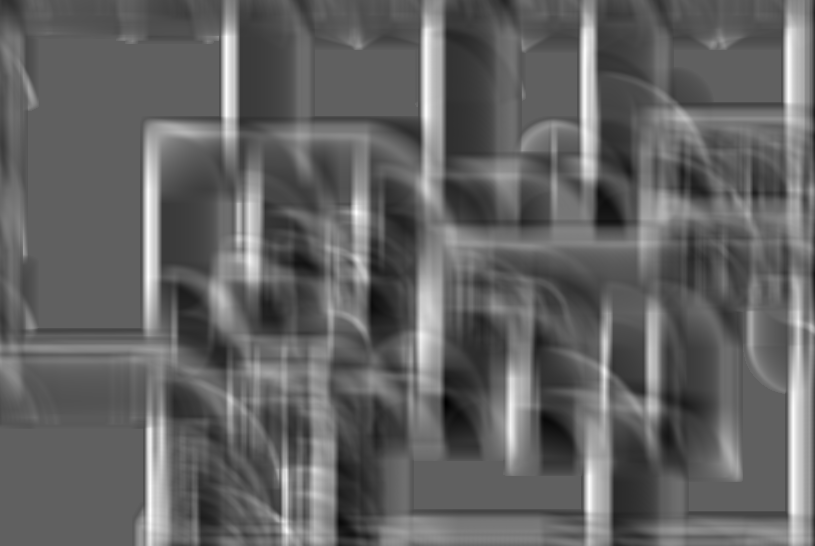
\includegraphics[width=0.8\textwidth]{TMAN1Correlation}
	\caption{Correlation matrix of \textit{A\_N1\_C}.}
	\label{fig:TMAN1Correlation}
\end{figure}

As shown on figure~\ref{fig:TMAN1Correlation}, the template correlates with a lot of objects in the image, like the walls. Instead of doors that will be recognised, the algorithm returns a lot of false positives and only one true positive.

\begin{figure}[H]
	\centering
	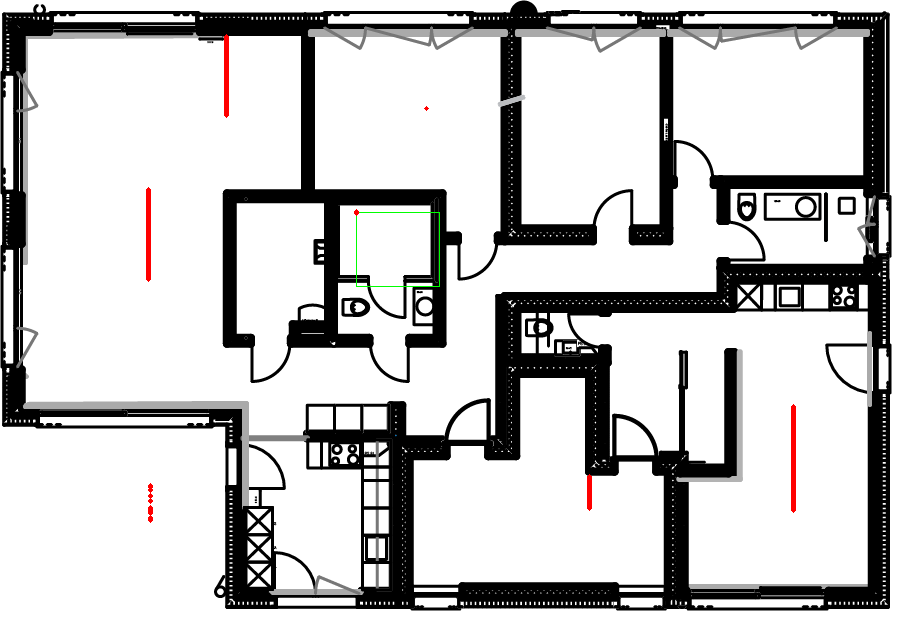
\includegraphics[width=0.8\textwidth]{TMAN1Result}
	\caption{Image \textit{A\_N1\_C} with detected doors.}
	\label{fig:TMAN1Result}
\end{figure}

This over-correlation can also be seen in figure~\ref{fig:TMAN1Result}, which shows the result of the component analysis. The red areas are the marked bright spots of the correlation matrix. Only one door in the middle of the plan is marked close to its location. This door is counted as true positive, even if the location does not perfectly fit.

\begin{figure}[H]
	\centering
	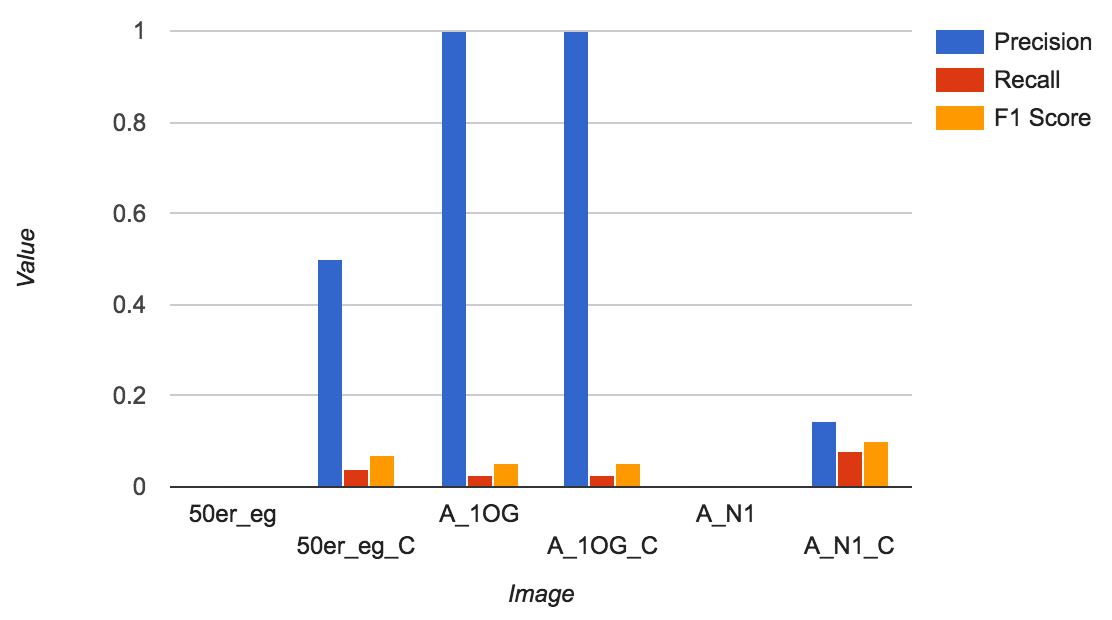
\includegraphics[width=1.0\textwidth]{TMResultDiagram}
	\caption{Results of the template matching experiment.}
	\label{fig:TMResultDiagram}
\end{figure}

This behaviour is also recognisable in the result graph (Figure~\ref{fig:TMResultDiagram}). The precision is very high, if something was detected. This is attributable to the fact, that very few positives have been detected. Recall instead is very low, because of the same reason. If no positives are recognised, whether \textit{true} or \textit{false}, the recall is very low. This is also reflected by the F1 score, which is nearby zero.

Interesting to mention is, that over all floor plans, the cleaned version (\textit{NAME\_C}) is better for the template matching, than the original image. But even the results of the clean versions are very poor.

We think that this bad result arose, because the template matching algorithm is not scale or rotation invariant. This leads to very few true positives. On the other hand, the correlation matrix shows, that the doors correlated with every straight wall on the plan. This could be a problem of the very common shape of doors.

\paragraph{Oriented FAST and Rotated BRIEF (ORB) OpenCV}
\label{sub:ImpORB}

As you see in the results of the template matching method (Section~\ref{sub:ImpTemplateMatching}), the scale and rotation variance of the algorithm delivers very bad results. The idea with ORB is to use an algorithm for object detection, which is rotation and scale invariant.

We use the algorithm implemented in \textit{OpenCV 3.1}. ORB also takes a template image $T$ and tries to find the objects in the image $I$. But ORB tries to find scale and rotation invariant features on the template image $T$. These feature are used to run the detection (Section~\ref{sub:ORBAlgorithm}). 

For our tests, the same template $T$ is used, as for template matching (Figure~\ref{fig:DoorTemplate}).

After implementing the algorithm, we recognized, that it was not able to detect any objects on the images. A visualisation of the features of our template image $T$ showed, that zero features have been detected in our image. Our investigations lead us to the conclusion, that the \textit{nFeatures} parameter of the ORB algorithm, was to low.

We tried to increase this feature count, but then realised, that it is not possible to set parameters for detectors in OpenCV 3.1. The problem is that the method, to read and write algorithm parameters, is implemented in the Java wrapper, but is missing in the C++ implementation (see \citep{orb}).

\paragraph{Oriented FAST and Rotated BRIEF (ORB) JavaCV}
\label{sub:ImpORBJVCV}
We then tried to use JavaCV to be able to access all parameters. The difference to OpenCV's method call is that each parameter can be specified. The problem with that approach was that the matrices used for JavaCV and OpenCV are different. Therefore, we had to copy the whole image, process it and then copy it back into the old matrix. To do this efficiently we had to use a buffer, or do it manually by hand. Both of those options took a lot of time as well as lot of memory and the buffer usually ran out of memory with larger images. At the same time, we had a different approach with the Cascade classifier in the pipeline, which looked a lot more promising. Therefore, this idea was put on hold and as the cascade classifier turned out very promising, it was never actually completely implemented.

\subsubsection{Cascade classification}
\label{sub:ImpCascadeClassifier}
The following section describes the cascade classifier algorithm to detect doors and other objects on the floor plan. After a short introduction, we will discuss the results and improvements of the different iterations of the algorithm training.

The cascade classifier is used for object recognition of doors, windows and other objects that are important for the room detection and zone identification. This algorithm is a machine learning algorithm that has to be trained with positive and negative images. The resulting learned parameters are saved in an XML file (Section~\ref{sub:CascadeTraining}). In the next section, the implementation process is described as well as all the experiences we made during this project.

The algorithm itself is trained with positive and negative images. It took multiple iterations to get to the trained classifier, we now use in the project. Each iteration differs by the parameters we have set during the training stage and the images we trained with.

\paragraph{Iteration 1 (CC\_T1)}
\label{sub:CCT1}
The first iteration of the training was to test out the capabilities of the cascade classifier. The results were not satisfying, but at least we were able to recognise something. We used a window size of \textit{32x24} and about \textit{20} positives samples and \textit{5} negative images. The positive images were a mix between floor plans of the customer and floor plans found on the internet. Negative images were original floor plans, where the object to train was removed.

\begin{figure}[H]
	\centering
	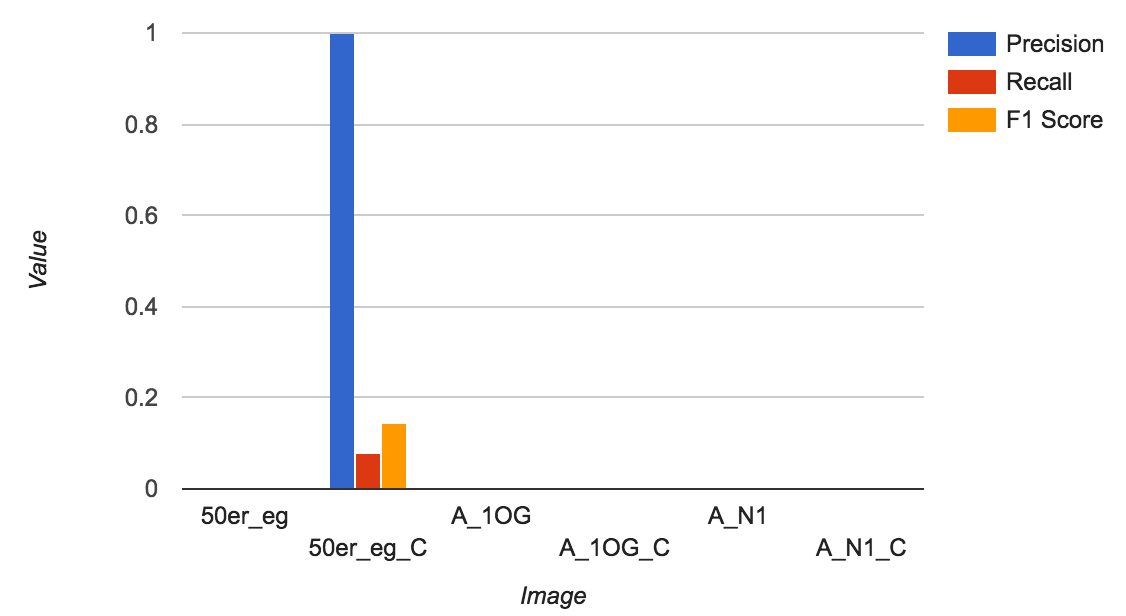
\includegraphics[width=1.0\textwidth]{CCT1Result}
	\caption{Results of the first cascade classification iteration.}
	\label{fig:CCT1Result}
\end{figure}

Figure~\ref{fig:CCT1Result} shows, that the trained classifier could not really find any doors on most of the floor plans. But if something was found, the precision is very high. This showed us that cascading classification is able to detect objects on a floor plan, but we needed to to detect more objects.

\paragraph{Iteration 2 (CC\_T2)}
\label{sub:CCT2}

Regarding iteration 1, we decided to increase the amount of positive samples to train more variations of doors. The second improvement was to lower the window size to \textit{20x20}. This lead to a better recognition of doors on floor plans with a low resolution. This is because the window size defines the lowest object size, which can be recognised by the cascade classifier.

\begin{figure}[H]
	\centering
	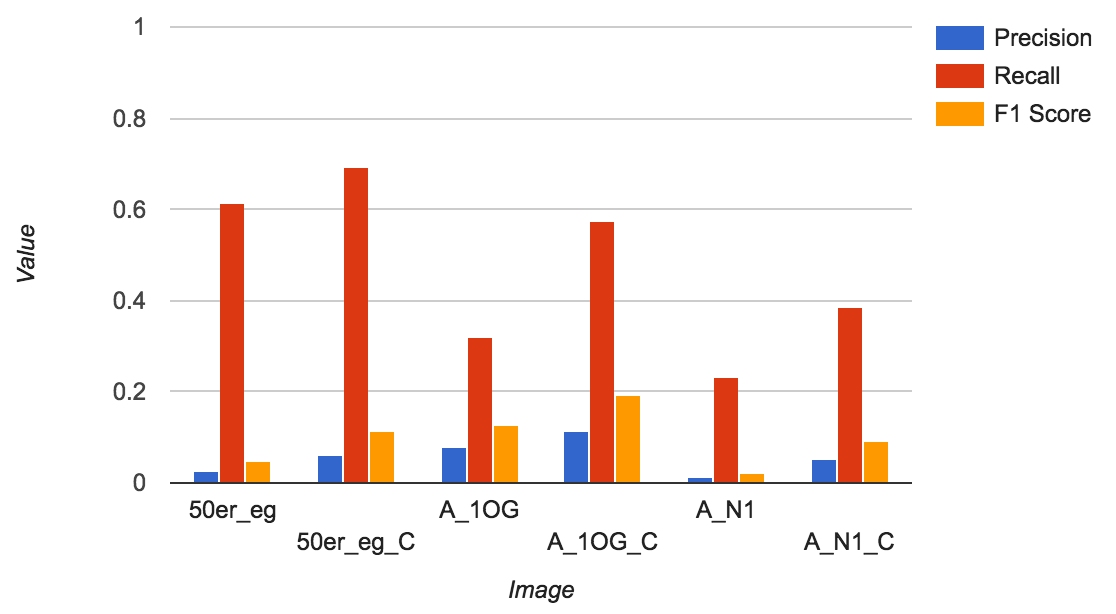
\includegraphics[width=1.0\textwidth]{CCT2Result}
	\caption{Results of the second cascade classification iteration.}
	\label{fig:CCT2Result}
\end{figure}

With this modifications, it was possible to detect much more objects on a plan then in iteration 1. The downside of this was, that the classifier was very inaccurate. There are very few true positives recognised, but a lot of false positives, which leads to a low precision (Figure~\ref{fig:CCT2Result}.

\begin{figure}[H]
	\centering
	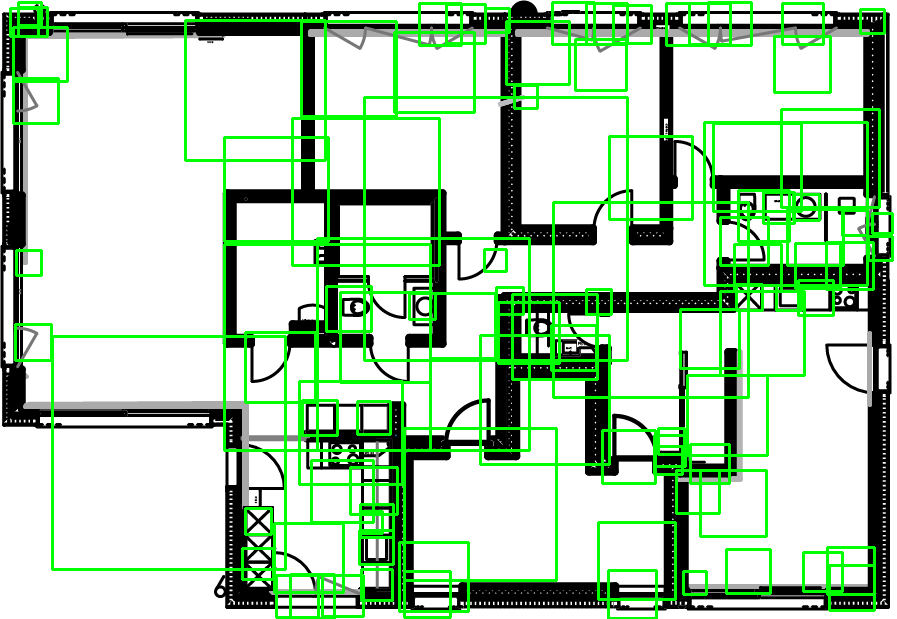
\includegraphics[width=1.0\textwidth]{CCT2ExampleAN1}
	\caption{Example of the second cascade classification iteration.}
	\label{fig:CCT2ExampleAN1}
\end{figure}

Figure~\ref{fig:CCT2ExampleAN1} shows an example of how the second iteration was performing. Nearly every element on the floor plan is detected as door. This lead us to the conclusion, that the door is trained with too few features, like the ORB method did (Section~\ref{sub:ImpORB}).

\paragraph{Iteration 3 (CC\_T3)}
\label{sub:CCT3}

To increase the features which can be detected on the positive samples, the decision was made to add a thickening to the trained floor plans. This thickening was also applied to the test images with the same parameters.

\begin{figure}[H]
	\centering
	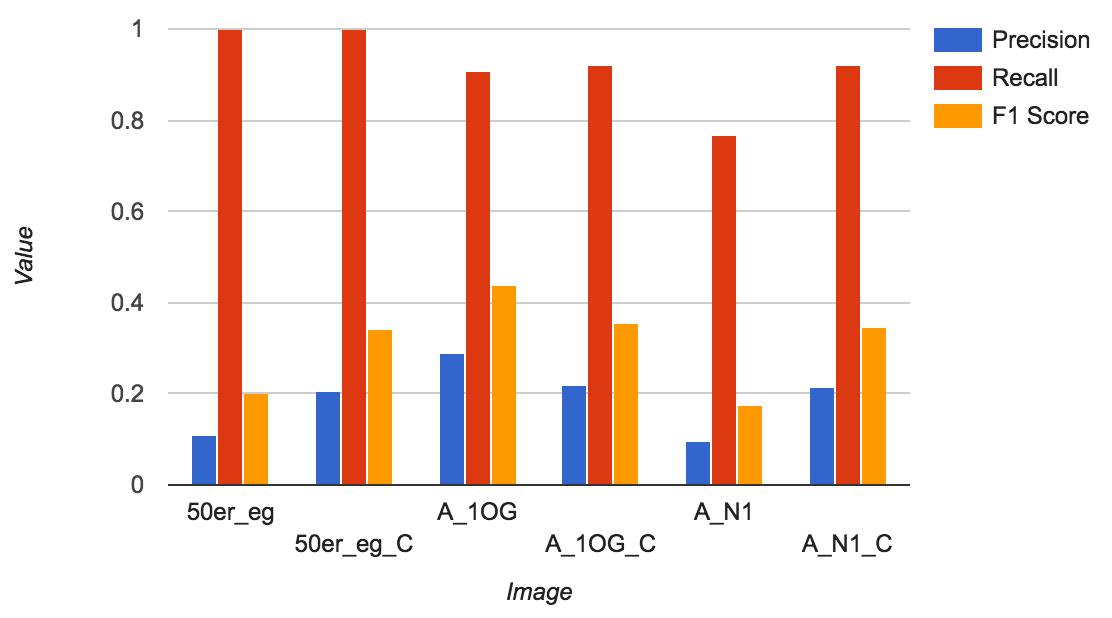
\includegraphics[width=1.0\textwidth]{CCT3Result}
	\caption{Results of the third cascade classification iteration.}
	\label{fig:CCT3Result}
\end{figure}

As seen on figure~\ref{fig:CCT3Result}, the precision slightly increased to iteration 2 (Figure~\ref{fig:CCT2Result}). This directly leads to a better F1-Score, because there were more true positives found in the images.

But the F1-Score is still very low, because a lot of the found images are not doors (false positive).

\paragraph{Iteration 3 with polygon matching (CC\_T3\_PolyDP)}
\label{sub:CCT3PolyDP}
\label{sub:PolyDP}

As improvement, we tried to use the cascade classification together with another method, which would classify the huge amount of positive images and filter out the false positives. The second method is called contour matching. It is a method to compare two shapes and get a value, which represents the difference between the two shapes.

\begin{figure}[H]
	\centering
	\subfloat[Template door]{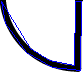
\includegraphics[width=0.3\textwidth]{PolyDPTemplate}\label{fig:PolyDPTemplate}}
	\hfill
	\subfloat[Matched door]{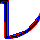
\includegraphics[width=0.3\textwidth]{PolyDPMatch163}\label{fig:PolyDPMatch163}}
	\hfill
	\subfloat[Matched door]{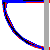
\includegraphics[width=0.3\textwidth]{PolyDPMatch41}\label{fig:PolyDPMatch41}}
	\caption{Shape matching template and matches.}
	\label{fig:ShapeDistanceMatching}
\end{figure}

To get the a template shape, we analyse the contours of the template image $T$ from the template matching method (Section~\ref{sub:TemplateMatching}). The largest contour on the template image (marked in blue on figure~\ref{fig:PolyDPTemplate}) is used as a template shape.

Now this shape detection is processed on every area, which the cascade classification has marked as positive. With the information of the largest contour, it is possible to calculate the distance to the template door. If both shapes have the exact same shape, the distance will be zero.

To filter out false positives, we have set a threshold, which only shows the areas, which match with a lower value than that of the threshold.

\begin{figure}[H]
	\centering
	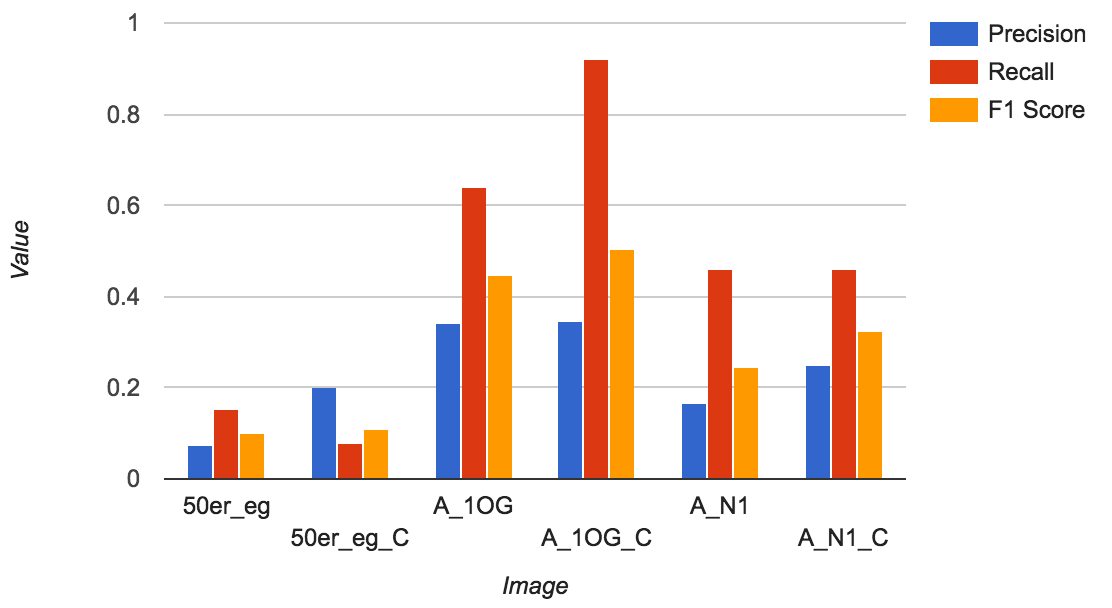
\includegraphics[width=1.0\textwidth]{CCT3PolyDPResult}
	\caption{Results of the third cascade classification experiment with shape matching.}
	\label{fig:CCT3PolyDPResult}
\end{figure}

To stack multiple detection methods behind each other was not as effective as we thought. As shown on figure~\ref{fig:CCT3PolyDPResult}, the F1-Score was on some images increased and on some decreased. This has to do with the template image $T$. It is very specific for one plan and if the doors do look a bit different on the plan, the contour will not match.

An advantage of this method is, that the amount of positive objects is decreased, because of the second filter method. But this also effects the recall on most of the images.

\paragraph{Iteration 4 (CC\_T4)}
\label{sub:CCT4}

After extensive research on how to improve the cascading classification method, we found an interesting blog post, which accurately describes how to get the best result from the training \citep{ball}. We realized, that the positive and negative sample ratio was not good for training small pictures like doors. In the previous iterations, we used a $2:1$ ratio, but it was recommended to use a $1:1$ ratio or higher.

We then decided to split up the large negative samples into very small pieces, to generate more negative images to train with. In the end we used about 600 positive samples and 600 negative samples.

\begin{figure}[H]
	\centering
	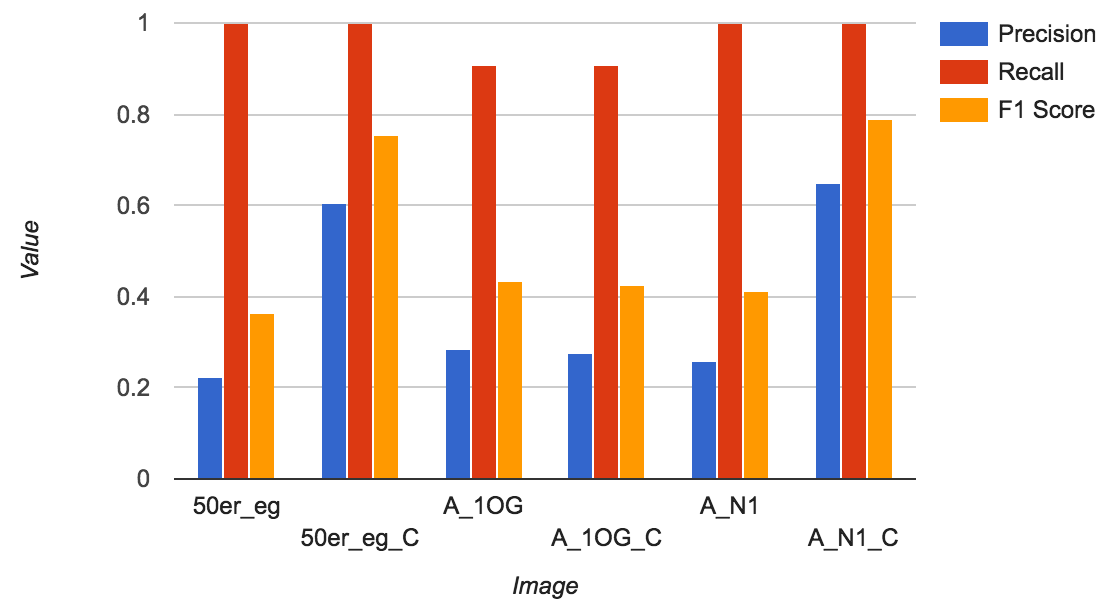
\includegraphics[width=1.0\textwidth]{CCT4Result}
	\caption{Results of the fourth cascade classification iteration.}
	\label{fig:CCT4Result}
\end{figure}

Actually, we used the same pictures like before, but the negative images have been cut into pieces. But this difference was a success as shown on figure~\ref{fig:CCT4Result}. The F1-Score is higher then ever before on every image. It was still not good enough, because there were some false positive detected, but not as much, as in previous iterations.

\paragraph{Iteration 5 (CC\_T5)}
\label{sub:CCT5}

In iteration five, we tried to improve the precision of the object detection, which was alright in iteration four (Section~\ref{sub:CCT4}), but still not good enough to use it in this project.

To increase the precision, we used even more negative samples to have a positive to negative sample ratio of $1:3$. As in iteration four, we used the big negative floor plans and cut them into very small pieces. In the end we used about 600 positive and 1500 negative images to train the classifier.

\begin{figure}[H]
	\centering
	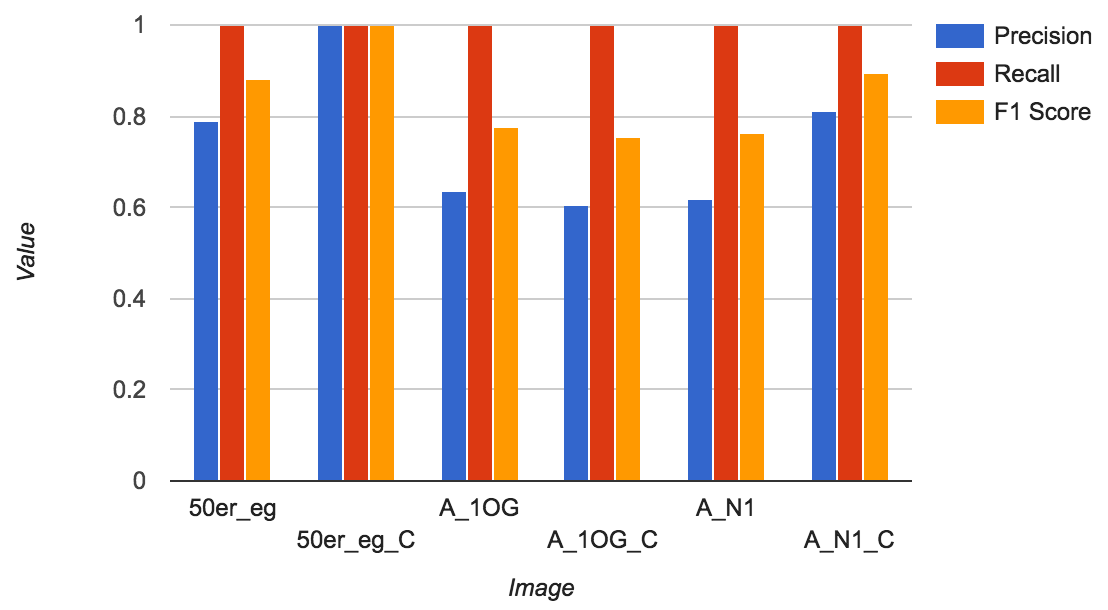
\includegraphics[width=1.0\textwidth]{CCT5Result}
	\caption{Results of the fifth cascade classification iteration.}
	\label{fig:CCT5Result}
\end{figure}

The results (Figure~\ref{fig:CCT5Result}) looked great. There were only very few false positives detected and, nearly all of the positives. The results seen in figure~\ref{fig:CCT5Result} originate from a test with fixed detection parameters. If we decrease the parameter \textit{minNeighbors}, the precision increases drastically. \textit{MinNeighbors} specifies how many neighbors each detected object should have, to retain in the result set.

\begin{figure}[H]
	\centering
	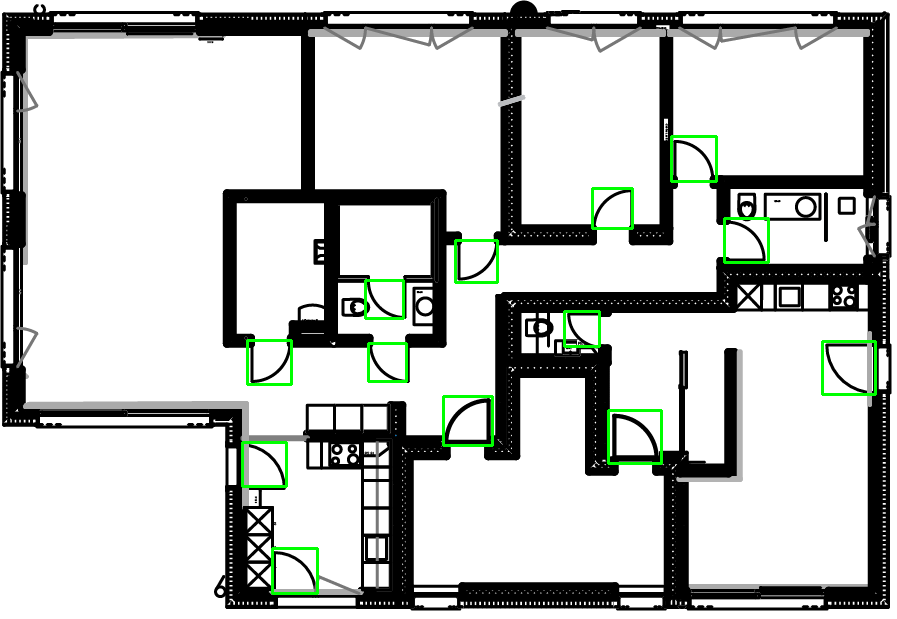
\includegraphics[width=1.0\textwidth]{CCT5ExampleAN1}
	\caption{Example of the fifth cascade classification iteration.}
	\label{fig:CCT5ExampleAN1}
\end{figure}

By default we use \textit{minNeighbors} with value $3.0$, but on some plans it is better to use a lower value. On the plan \textit{AN\_1} for example, it is better to use a value of 8.0 to get only the doors (Figure~\ref{fig:CCT5ExampleAN1}).

We currently use this training iteration for the door detection in the software. It is not perfect, but it is accurate enough to use and detect most of the doors.

\paragraph{Results}
\label{sec:ResultsCascade}
In this section, we will summarise the results of the cascading classification iterations and discuss the general improvements between each step.

\begin{figure}[H]
	\centering
	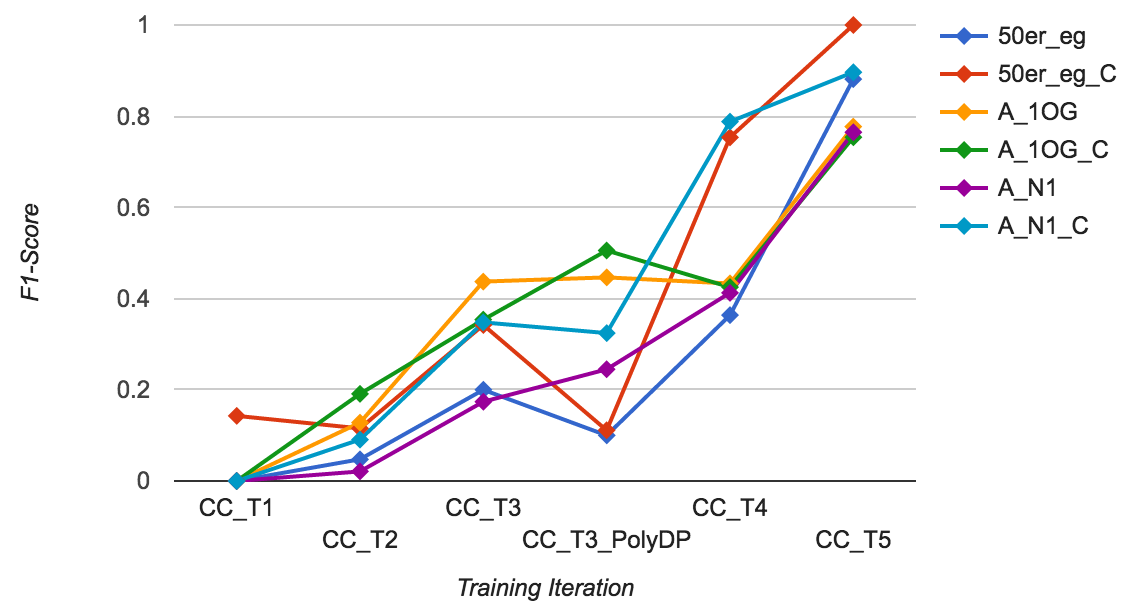
\includegraphics[width=1.0\textwidth]{CCF1ScoreGraph}
	\caption{F1-Score results of the floor plans.}
	\label{fig:CCF1ScoreGraph}
\end{figure}

Figure~\ref{fig:CCF1ScoreGraph} shows the F1-Score of each floor plan, over each training iteration. With more samples to train the classifier, the results increased over each training. Only the \textit{CC\_T3\_PolyDP} training was a retrogressive step, because the stacked filter system was too restrictive and rejected even true positives. In step \textit{CC\_T5}, all tested floor plans achieved an accuracy (F1-Score) over 75 percent, which was enough to use it in the gap closing algorithms (Section~\ref{sub:GapClosing}).

Another interesting graphic is the comparison between the performance of the original and cleaned floor plans. Figure~\ref{fig:CCF1ScoreGraphOCAverage} shows the averaged F1-Score of the original and cleaned floor plans, over each iteration. The cleaned floor plans always perform better then the original ones. This has to do with noise on the plans like furniture, text or markings, which are falsely classified as objects. This behaviour is intended.

\begin{figure}[H]
	\centering
	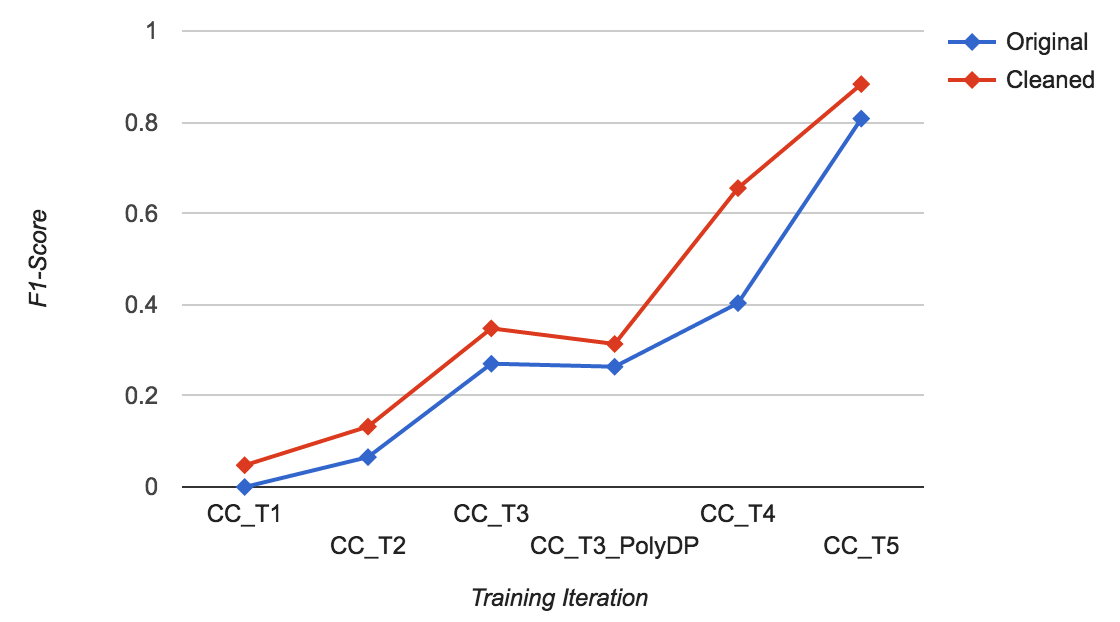
\includegraphics[width=1.0\textwidth]{CCF1ScoreGraphOCAverage}
	\caption{Averaged F1-Score of original (blue) and cleaned plans (red).}
	\label{fig:CCF1ScoreGraphOCAverage}
\end{figure}

Interesting is the difference in iteration 4 (\textit{CC\_T4}), because the cleaned floor plans have drastically increased their accuracy, but the original ones only marginally. This has to do with the false positive detection count. There is much more noise in the original plans, which leads to a higher count of false positives. Only when we increased the negative sample count to 1600, also the original plans could make a big step and double its accuracy.

The graph shows that it is recommended to do a clean up before processing the image. This includes removing unnecessary walls, furniture and markers.


\subsubsection{Gap closing}
\label{sub:GapClosing}
In this section, gap closing will be discussed. There are two different types of gap closing in this project. There is the outer-wall gap closing. This is mainly a gap closing of all the existing windows. This is important to circumvent the rooms to the outside of the house. The second part of gap closing is the door closing. It is important as per definition all rooms are separated by a door. By closing the door gap, the room finding algorithm will then be able to easily find each room.
\paragraph{Edge door closing}
The edge door closing algorithm was the first algorithm that was implemented to solve the problem of closing doors. The idea behind it was, that in the area of any found door with the cascade classifier, there would be a rectangle of corners that represent the edges of the walls where the door is attached to. Therefore, an algorithm was implemented, that detected those corners and then tested if there was an actual rectangle within that area.

The idea is that on the area a door is found there is usually no other rectangle of corners other than the door frame itself. This assumption is made after the morphological cleaning is done, therefore most noise that could have created a rectangle of corners should have been extinguished. On the image of the walls, the algorithm performs a Corner Detection (see section~\ref{subsubsec:HarrisCornerDetection}). This results in an image that represents all locations that are likely to be a corner with white pixels. Usually, one corner is detected in the form of several white pixels. To find the exact position of this corner the algorithm uses Point Clustering (see section~\ref{sec:PointClustering}) to find its center. After all corners and doors are found, the door gap closing algorithm (see section~\ref{sec:DoorGapAlgorithm}) kicks in. It finds the rectangles that create the door frame within the area of the detected door and some additional margins. This margin was added, as the detected door symbol usually does not contain the door frame and the wall enclosing it, and therefore does not have the corners within the original detection square.
When a door rectangle was found, it was filled with black color. This closed the gap on the image.

\begin{figure}[H]
	\centering
	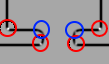
\includegraphics[width=0.6\textwidth]{CornerNotFound}
	\caption{This image shows the result of a corner detection. Blue circles represent corners that should have been found but were not. Red circles represent corners that were found by the Harris corner algorithm. In this image the door frame rectangle can not be found because two out of four corners are missing.}
	\label{fig:CornerNotFound}
\end{figure}

A big problem with this approach was, that some of the corners on floor plans were too round. As soon as one corner of the needed four was not detected the algorithm wouldn't close the gap. Additionally, if a wrongly detected door was enclosing a room within itself. The whole room was identified as a gap and therefore filled. This was a rare occurrence. This algorithm didn't deliver very good results,due to its very restrictive conditions.

\paragraph{Simple door closing}
\label{sub:SimpleDoorClosing}
As a result, an easier solution for gap closing was created. It again uses the squares with the location of the found doors. It makes use of the fact that on the image where all the noise was removed, the symbol of the detected door is erased. All that is left within the square, are walls. Due to the fact that the found door will always be where the gap for a door is, there have to be two ends to a wall as well. The algorithm connects those walls with a simple combination of erosion and dilation.

\begin{figure}[H]
	\centering
	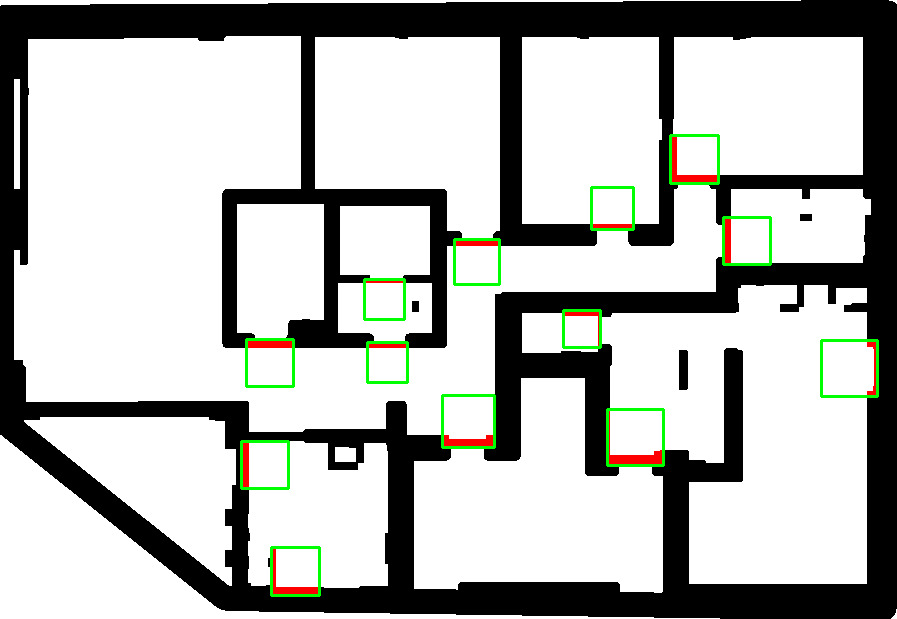
\includegraphics[width=1.0\textwidth]{SimplifiedGapClosingAN1}
	\caption{Simplified gap closing visualised on the plan AN\_1. The red areas represent the closed gaps.}
	\label{fig:SimplifiedGapClosingAN1}
\end{figure}

The lines of the wall within that square are eroded until they connect and then dilated back to their original size. The difference is that the gap is now filled and looks like it is part of the wall (Figure~\ref{fig:SimplifiedGapClosingAN1}). This algorithm doesn't have to deal with undetected corners. It will also not change any existing walls with no gaps that are within one of the squares. These walls will just be expanded and then resized to their original size. The only problem that was found with this algorithm, was that if the erosion size was too big, the whole square will be filled. This is obviously not intended and therefore incorrect.

\paragraph{Door closing comparison}
\label{sub:DoorClosingComparison}
In this section both of the algorithms are compared to each other. It will describe how effective they were, and explain the results.

\begin{figure}[H]
	\centering
	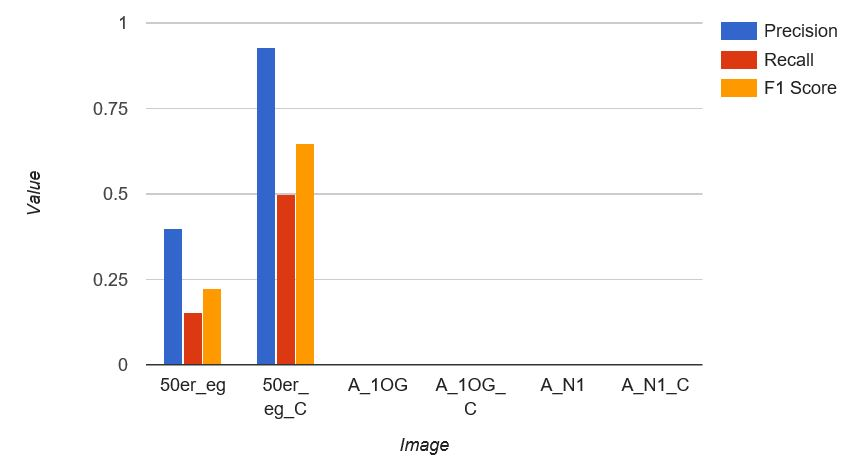
\includegraphics[width=1.0\textwidth]{pointDoorClosing}
	\caption{Precision, Recall and F1-Score for all images processed with the edge door closing algorithm. }
	\label{fig:pointDoorClosing}
\end{figure}

As shown in the figure \ref{fig:pointDoorClosing}, the images A\_1OG and A\_N1 do not have any scores at all. The problem for image A\_1OG is, that due to the structure of the doors within this plan, the algorithm can not find 4 corners to connect. The door frame is already closed, as the door symbol itself had a "wall" connecting the enclosing walls. The problem with the image A\_N1 is that there are never four edges detected for one door, because at least one of the supposed corners is too round. It is not detected as a corner and therefore no door closing is done. For the last plan, the cleaned version shows decent results, since the precision is at 90 percent. The problem is that not all doors are correctly detected and provide the four corners. Therefore the recall is only at 50 percent.

\begin{figure}[H]
	\centering
	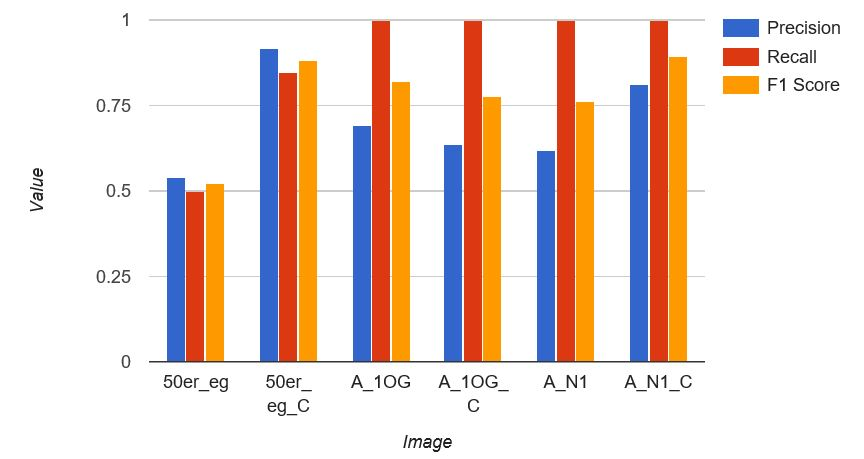
\includegraphics[width=1.0\textwidth]{simpleDoorClosing}
	\caption{Precision, Recall and F1-Score for all images processed with the simple door closing algorithm. }
	\label{fig:simpleDoorClosing}
\end{figure}

In comparison, the simple door closing algorithm shows much better results. The precision for all images is comparably low. This is due to the fact that the cascade classifier has identified more doors than are actually on the map. All of those additional doors found count as false positives. Important to note is that this does not impact the algorithm in a strong manner. Almost all of those false positives have no negative effect on the future algorithm, as they usually draw over a present wall. This has no effect on the resulting image. This shows especially in the recall, where in two out of the three images all doors are closed.
For this door closing algorithm a good recall is the most important number as closing of false positives seldom real impact on the image itself.

As can be seen from the results of both of the algorithms, the second algorithm is a lot more robust to noise and like rounded corners and already closed doors. It does not need to identify any corners to work and closed doors are treated like a preexisting wall. This shows an extreme improvement for door gap closing on any image and has almost no drawbacks to our current knowledge. With the first algorithm, the implementation is very restricted to good conditions. The simple door closing algorithm in contrary will work under almost all circumstances and was therefore used for the final workflow.

\paragraph{Wall closing}
\label{sub:WallClosing}
As for wall closing, there were two different approaches tested. The most obvious approach was to find all the windows with object detection and then close those gaps. The problem with this attempt was, the way windows are represented in architectural floor plans changes on most plans. The few tests done showed very bad results and therefore it was decided that there had to be a different method to close the windows.

This new algorithm finds the outer walls by finding the convex hull for the polygon of the outside walls. It then closes them by drawing a line, that represents the closed wall, along the outer hull. This way, the outer bounds are all enclosed.
The algorithm will first find all the contours as described in section~\ref{sub:FindContoursTheory}. Based on those contours it will find the convex hull (see section~\ref{sub:ConvexHull}) of the outer polygon from all the drawn contours. This leads to the exact convex hulls of the outer walls. Sometimes there are outliers from the wall that have no connection to any room and would therefore create additional rooms. To try and prevent this, the polyDP (see section~\ref{sub:PolyDP}) was implemented. It can straighten out lines and therefore reject outliers of walls. This helped to create a more realistic outer wall.
\subsubsection{Room detection}
\label{sub:RoomDetection}
In the following section, the room detection used in the third workflow will be discussed. It features a short description of how each algorithm was used for room detection and then discusses the different results.
\paragraph{Connected components}
\label{sec:ConnectedComponents}
To detect the rooms in workflow three, the connected components algorithm was used. This algorithm is described in detail in section \ref{sub:ConnectedComponentAnalysis}. What it does is, that it creates groups of white pixels that are connected to each other. Each group of white pixels represents its own room. The connected component search is done after all noise removal, object detection and gap closing algorithms are run. An additional heuristic implemented is, that all rooms connected to the border of the image are not recognized as rooms. It is expected that any building has an outer wall, therefore no room can touch the border of the image.

In the figure \ref{fig:RoomDDResult}, the numbers for Precision, Recall and F1-Score for room detection with the connected components algorithm are listed. All of the tests were done by our team and a detailed description can be found in the file \textit{Evaluation.odf}, which comes with this work. Any information to replicate the tests can be found within this document. The tests resulting in this graph were done without any user interaction other than adjusting the algorithm parameters. There was no manual deletion of noise or closing of gaps by hand.

As seen in figure \ref{fig:RoomDDResult}, the results for the two uncleaned images are much worse than for the cleaned ones. This is due to the fact, that the outer wall closing does not work properly on an uncleaned image. This messes up most rooms, as a lot of windows are not closed. Unclosed windows create wrong rooms and have a negative effect on all three bench marks. The cleaned versions show a high precision with all of them being around 90 percent. This shows that the room detection works really good even without any user interaction. The high recall value shows, that no matter how complicated a plan is, or how many rooms a plan has, most of the rooms are still correctly detected. Any of these values can be further improved if the user takes more time to find better parameters for the algorithm. But these results should show a good representation of a daily detection, where the user will not take minutes to find the best possible parameter. Instead, he will correct minor mistakes afterwards by hand, which is more time efficient.

\begin{figure}[H]
	\centering
	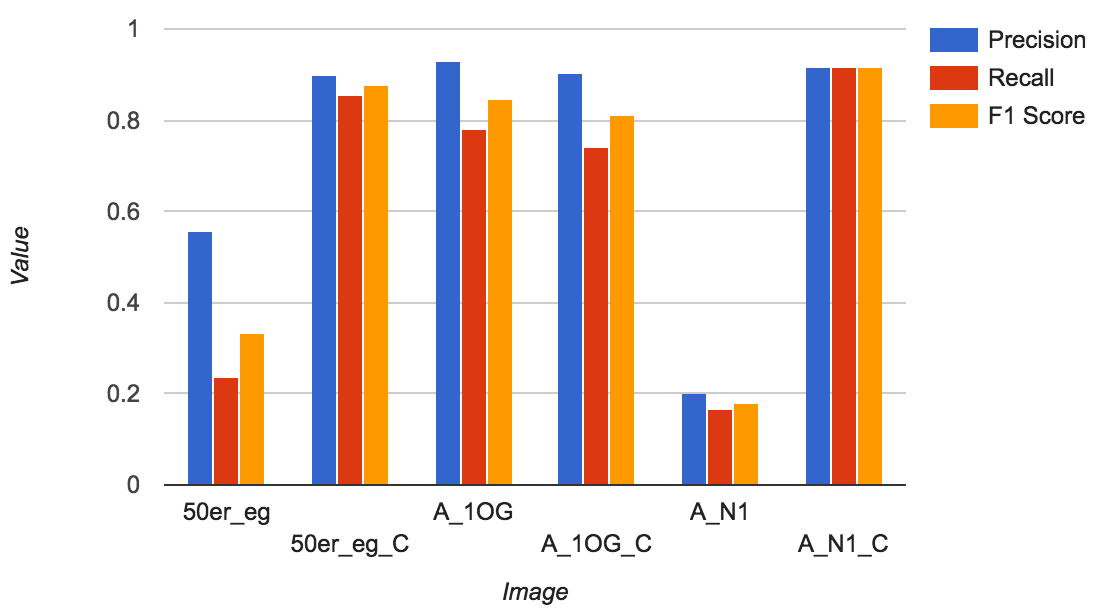
\includegraphics[width=1.0\textwidth]{RoomDDResult}
	\caption{This graph represents precision, recall and F1-score for all tested images. Each image was tested with an uncleaned and a cleaned version. The letter "C" represents the cleaned image version. In the tests represented, there was no additional cleaning of the images with the tools available within the editor. }
	\label{fig:RoomDDResult}
\end{figure}

The following figure \ref{fig:RoomDDResult} shows the results of the same tests as the ones done above. The difference is, that in these tests, the tester was able to use the tools provided within the editor. The figure shows precision of a 100 percent. This improvement, especially in the uncleaned plans, was created due to the fact that the editor can basically create a cleaned version of the plan. Therefore, even the "uncleaned" versions show high precision and recall. If taken enough time, all those bench marks could be at a 100 percent, as you can basically redraw the plan with the existing tools. But those tests had to be done within a considerable amount of time. Therefore, some of the plans do not have a recall of 100 percent.

\begin{figure}[H]
	\centering
	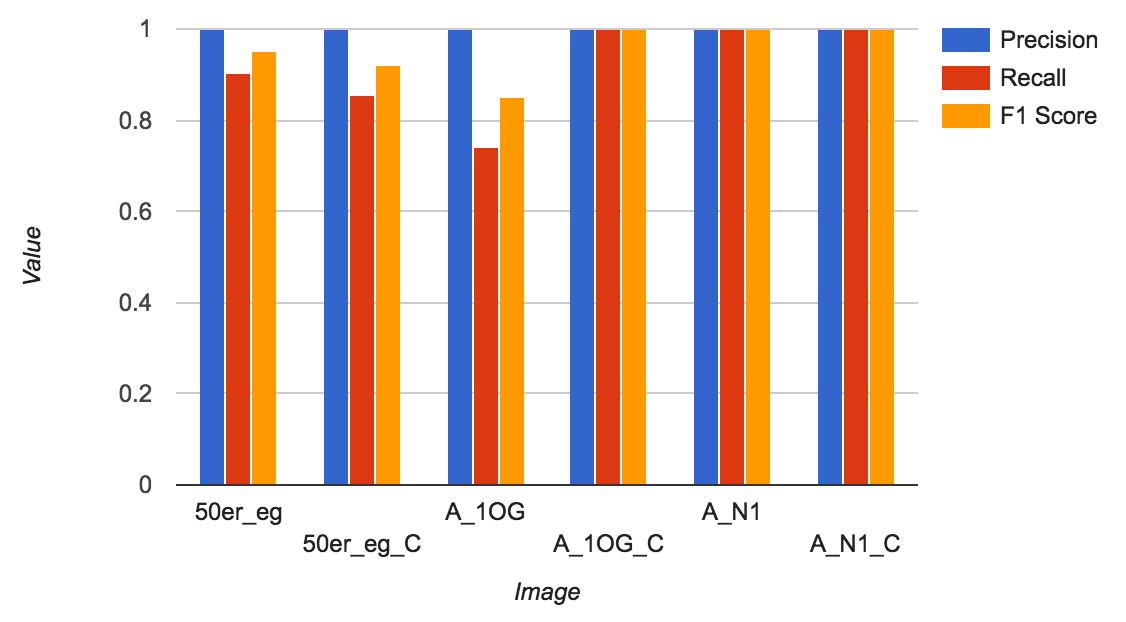
\includegraphics[width=1.0\textwidth]{RoomDDEResult}
	\caption{This graph represents precision, recall and F1-score for all tested images. Each image was tested with an uncleaned and a cleaned version. The letter "C" represents that the image is the cleaned version. In the tests represented, the tester did additional cleaning of the images with the tools available within the editor. These tools can create or erase lines. }
	\label{fig:RoomDDEResult}
\end{figure}

All of these bench marks discussed show how good the actual room detection works. But there is no comparison yet, what the improvements are compared to the old program used at the Planfabrik GmbH. As defined in the metrics, the whole process to detect the rooms was measured with clicks and time used to detect the rooms. This comparison with these values will be done just below.

As seen in figure \ref{fig:ClicksPerPlan}, the clicks or user input is far less than the amount needed with the old program. This comes from the fact, that algorithms find the room corners directly and do not need one click per corner. As seen, the amount of clicks needed stays about the same for each detection run. This shows, that the user input will be about the same no matter how complicated or how many rooms a plan has. The clicks used are mostly to adjust the parameters for the algorithms. This is fare less than most plans have room corners on them. Additionally, most tests with cleaning done by the user take some more clicks. But it is within a very small margin, compared to the run with no error correction. What can be said about this program is, that it generally takes less clicks than the old program. Not only that, but the bigger the plan, the fewer additional clicks it takes to process compared to the old program. 

\begin{figure}[H]
	\centering
	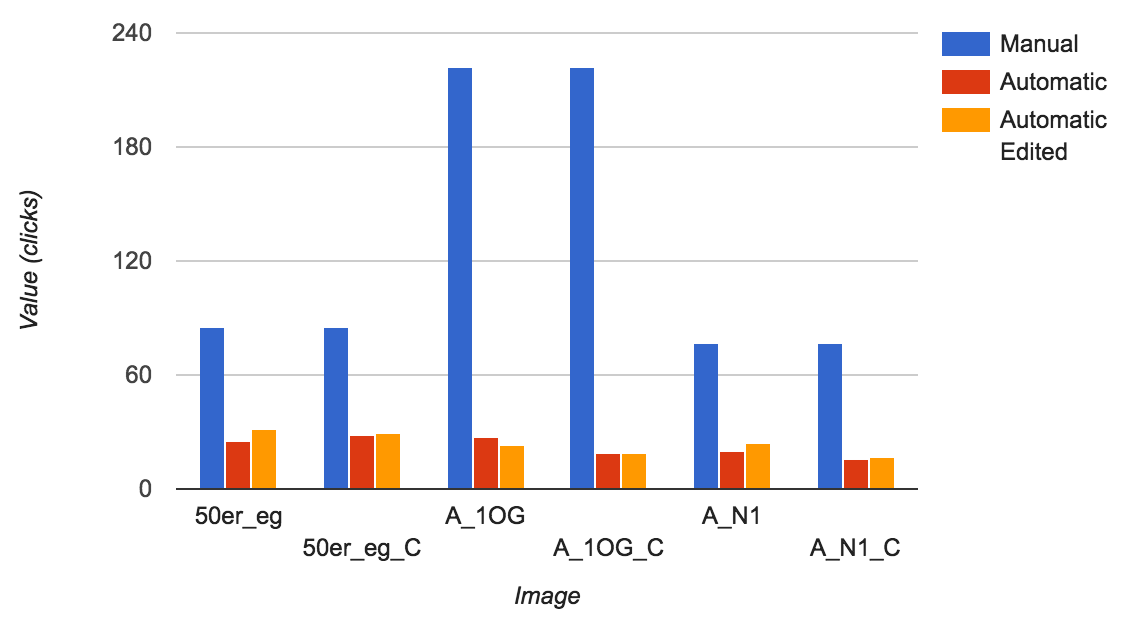
\includegraphics[width=1.0\textwidth]{ClicksPerPlan}
	\caption{This figure shows the clicks that were needed to fully process a plan. The blue bar represents the tests that were done with the old program within the Planfabrik GmbH. The red bar represents the tests without user editing of plans, while the orange bar represents with user editing.}
	\label{fig:ClicksPerPlan}
\end{figure}

The same was done in \ref{fig:TimePerPlan}, as in figure \ref{fig:ClicksPerPlan}. The difference is that figure \ref{fig:TimePerPlan} shows the time instead of the clicks needed. This graph indicates the same results as the other graph. It takes more time to find the rooms on a bigger plan when done with the old program. This program shows only small differences in time consumed, no matter which plan was tested. 

\begin{figure}[H]
	\centering
	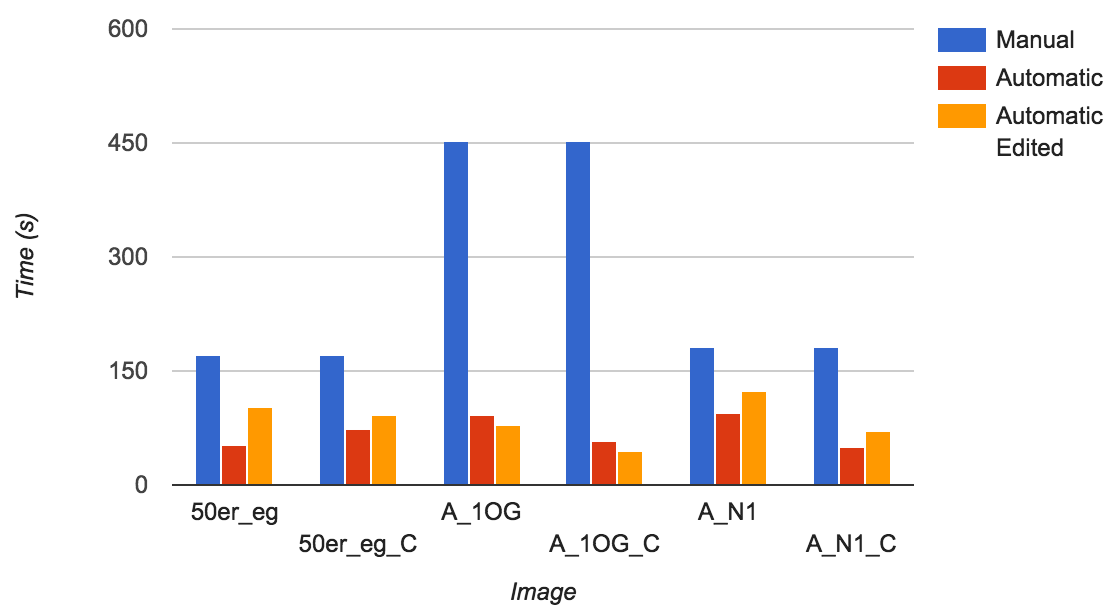
\includegraphics[width=1.0\textwidth]{TimePerPlan}
	\caption{This figure shows the time that was needed to fully process a plan. The blue bar represents the tests, that were done with the current process within the Planfabrik GmbH. The red bar represents the tests without user editing of plans, while the orange bar represents with user editing.}
	\label{fig:TimePerPlan}
\end{figure}

In general we can say, that this algorithm does solve the problem faster and with less user interaction than the old program.

\paragraph{Minimum room deletion}
\label{sub:MinimumRoom}
To improve the actual room detection, a simple heuristic was created. The problem was, that due to the fact that the wall closing algorithm was not perfect and other factors, very small rooms were detected, that were no rooms. This was so obvious that those detected rooms could not be a room itself, because they were more than a hundred times smaller than the biggest room.
To reject these rooms the program provides a factor, usually one percent, that the rooms to be removed have to be smaller than the biggest room of the house. This one percent is calculated on the area of both rooms and it is a measure that proved to be solid for all tested plans.

\paragraph{Result}
To test how accurate the room detection works, we analysed a floor plan and compared the results of the software with the values, which are stated on the actual plan. The test uses the plan \textit{50er} and \textit{50er\_C} and its \textit{BF} (\textit{Boden Fläche}) label as room size.

\begin{figure}[H]
	\centering
	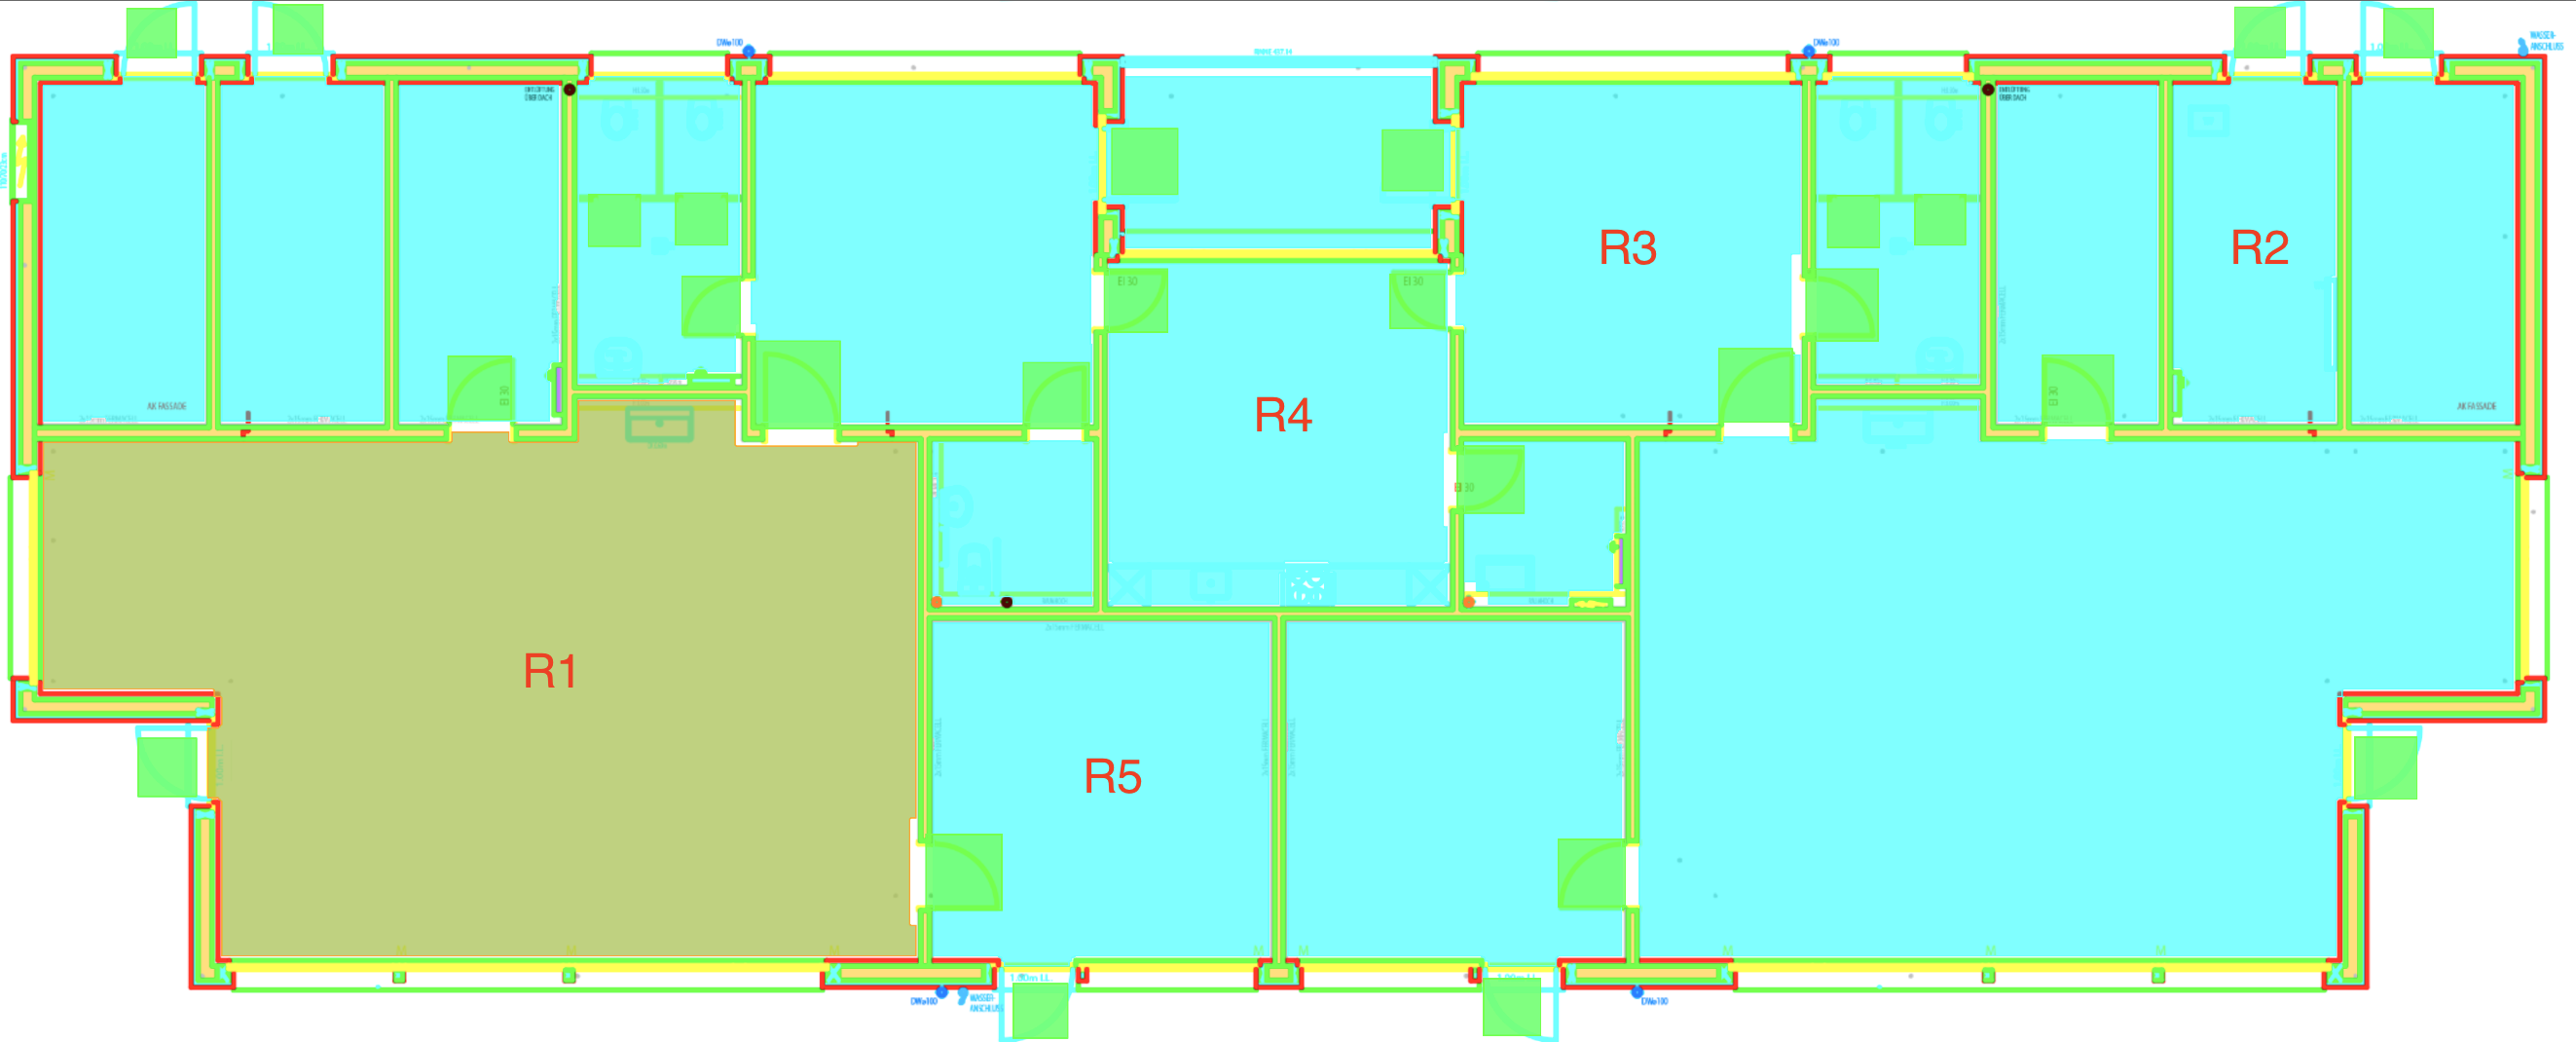
\includegraphics[width=1.0\textwidth]{50erRoomSize}
	\caption{This figure shows the 50er\_C room plan with the marked room polygons. For the accuracy test, the red marked rooms are used.}
	\label{fig:50erRoomSize}
\end{figure}

Only five of the rooms have been tested, because most of the rooms have the same size. We tried to use different room sizes to get a representative result of the accuracy. The rooms are marked in figure~\ref{fig:50erRoomSize} with a red label. The test was done with default small edits by the user, to simulate a real workflow.

\begin{figure}[H]
	\centering
	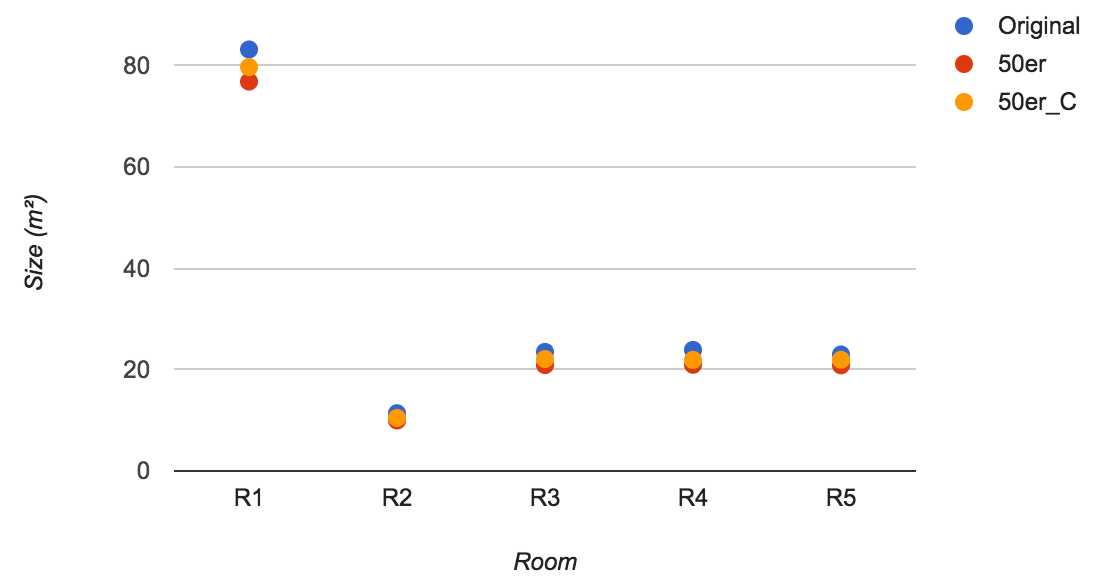
\includegraphics[width=1.0\textwidth]{50erRoomAccuracy}
	\caption{This figure shows the accuracy test results of the 50er\_C room plan in $m^{2}$.}
	\label{fig:50erRoomAccuracy}
\end{figure}

As shown on figure~\ref{fig:50erRoomAccuracy}, the detected room sizes are always smaller then the actual values. The larger the room, the bigger is the deviation in m$^{2}$. We think this is, because the algorithm is missing some areas at the doors and due to the inaccuracy of the ruler tool. With this tool, it is possible to set the distance relations and if this is done inaccurately, all room sizes will suffer from it.

\begin{figure}[H]
	\centering
	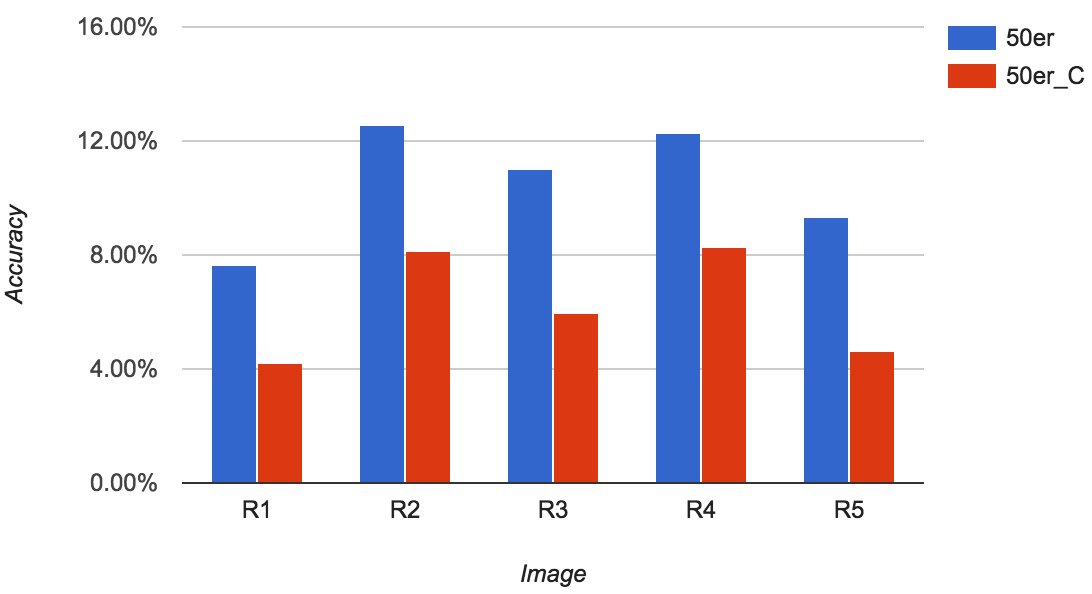
\includegraphics[width=1.0\textwidth]{50erRoomAccuracyPercent}
	\caption{This figure shows the accuracy test results of the 50er\_C room plan in percent.}
	\label{fig:50erRoomAccuracyPercent}
\end{figure}

The deviation is even stronger on original plans than on cleaned plans (Figure~\ref{fig:50erRoomAccuracyPercent}). We think this comes from the fact, that the cleaned plans have less noise on it, which could create interferences in the room polygons.

Our test showed that there is an average deviation of 10.55percent on original plans and 6.25 percent on cleaned floor plans.



\section{Theory}
\subsection{Information Segmentation}
\subsubsection{Erosion and Dilation}
\label{subsubsec:Erosion and Dilation}
In our project we need dilation to strengthen small features that we want highlighted, as well as to get rid of small details in the picture itself. We use it in early preprocessing, because together with the erosion it helps clean up pictures, in oder to further process them without too many interfering objects in the image. The main usage is to extract an image that features all the walls and has as few other lines on it as possible \citep{burger_burge_2016}.

For our project we use the binary grayscale erosion~\eqref{eq:GrayscaleErosion}.
The erosion uses the following principle to work.


\begin{equation}\label{eq:GrayscaleErosion}A \ominus B = \{ z\in E | B \subseteq A \}\end{equation}  
\begin{equation}\label{eq:StructuringElement}where: B_{z} = \{b+z | b \in B\} with \forall z \in E \end{equation}

$A$ is a binary image in the Euclidean space or an integer grid. The erosion is done with the structuring element $B$~\eqref{eq:StructuringElement} on the image $A$. The structuring element has to be a subset or equal to $A$, otherwise there will be no erosion. The mask $B$ will be applied to all pixels possible, if the mask fits on the center pixel of $A$, the value will be retained. Otherwise it will get deleted. This means, that only when $B$ is completely contained in $A$, values of pixels are retained.

Binary dilation uses the exact same process. The only difference compared to the erosion is, that the deletion of the pixel will not be setting pixel values to white 1, but to black 0. Both of those processes are inherently the same and can be summed up under the term morphological operation. Morphological operations are altering the image with a mask, as we did here for erosion and dilation.

\subsubsection{Geodesic Dilation}
\label{subsubsec:GeodesicDilation}

Geodesic dilation is an iterative morphological transformation for the reconstruction of marked foreground objects. Instead of the normal dilation (Section~\ref{subsubsec:Erosion and Dilation}) it uses a marker image $F$ which defines the starting points of the dilation, a mask image $G$ which defines the constraints of the dilation and a structuring element $B$ which describes the dilation itself.

For example the algorithm is used to reconstruct the area of the brightest points within a distance transformed image (Section~\ref{subsubsec:Distance transformation}). We used this for extracting and enhancing the room center points which then are used as marker points of the watershed marker image (Section~\ref{subsub:watershed}).

The geodesic dilation is defined as $D_{G}^{(n)}(F)$ where n is the iteration size and $F$ the marker with respect to the mask $G$. As a precondition $F$ is a subset of (or is included in) $G$: $F \subseteq G$.

There is no implementation in \gls{gloss:OpenCV} of this algorithm, so we did it ourselves. Following is a short overview of our implementation.
	
\begin{equation} \label{eq:geodesic_dilation_iteration}
\begin{gathered}
D_{G}^{(0)}(F) = F
\\
D_{G}^{(1)}(F) = (F \oplus B) \cap G)
\\
D_{G}^{(n)}(F) = D_{G}^{(1)}(D_{G}^{(n-1)}(F))
\end{gathered}
\end{equation}

Where:
\begin{itemize}[label=]
    \item $F$: is the marker image
    \item $G$: is the mask image
    \item $B$: is the structuring element
    \item $n$: is the iteration index
\end{itemize}

As seen in equation~\eqref{eq:geodesic_dilation_iteration}, a geodesic dilation with zero iterations is equal to the initial marker image. In the first iteration the marker image $F$ is dilated with the structural element $B$ and the result of that dilation is intersected with the mask image. This intersection limits the dilation to the marker constraints. After one iteration the next iteration uses the result of the last iteration as new marker image $F$.

The iteration stops as soon as the the difference (absolute array norm) between $F^{n}$ and $F^{n-1}$ becomes less then $\epsilon$ which in our case is 0.0001.

\subsubsection{Distance transformation}
\label{subsubsec:Distance transformation}
As well as the erosion and dilation, the distance transformation is a morphological operation. In our project it serves the purpose to find basins for the watershed algorithm. This is used to define the foreground picture. We will explain this further in the wathershed discussion.
It is used after preprocessing to find the center of what is supposed to be rooms. This algorithm is only used in combination with the watershed.

The algorithm that OpenCV uses is called cvDistTransform and uses an euclidean distance to calculate the output image. The input for this transformation is a binary image $I(u,v) = I(x)$ which will be separated into a foreground \eqref{eq:Foreground} and background \eqref{eq:Background} image.
\begin{equation}\label{eq:Foreground}FG(I) = {x | I(x) = 1}\end{equation}
\begin{equation}\label{eq:Background}BG(I) = {x | I(x) = 0}\end{equation}
The formula for the distance transformation of $I$, $D(x)$ itself is defined as:
\[D(x) :=\min_{x' \in FG(I)} dist(x,x') \]
It applies to any pixel $x = (u,v)$ of the input image. If the pixel is part of the foreground image $FG(I)$ then the result of the transformation $D(x)$ is zero. As said above, the distance formula $dist(x,x')$ is the euclidean distance \eqref{eq:EuclideanDistance} (also called $L_{2}-Norm$) between two pixels.
\begin{equation}\label{eq:EuclideanDistance}dist(x,x') = ||x - x'|| = \sqrt{(u - u')^2 + (v - v')^2}\end{equation}

Since the exact calculation with the euclidean distance takes a lot of computational power openCV uses the Chamfer-Algorithm instead. This algorithm runs two masks over the image. The first mask $M_{L}$ \eqref{eq:LeftMask} is run in a diagonal manner over the image, starting in the top left corner of the image. The second mask $M_{R}$ \eqref{eq:RightMask} does the same in reverse starting at the bottom right corner. Those masks are a matrix that represent the euclidean distance between the center and the pixels around it. Each mask only changes the pixels in the direction they are run through the image \citep{burger_burge_2016}. As a result, the masks look similar to the following ones:
\begin{equation}\label{eq:LeftMask} M_{L} = \begin{bmatrix} . & . & .\\ . & x & m_1 \\ m_2 & m_1 & m_2 \end{bmatrix}\end{equation}
\begin{equation}\label{eq:RightMask}M_{R} = \begin{bmatrix} m2 & m1 & m2 \\ m1 & x & . \\ . & . & . \end{bmatrix} \end{equation}

This all leads to the resulting effect shown in the image below (\citep{szeliski_2011} and \citep{distancetransform}).
\begin{figure}[H]
	\centering
	\includegraphics[width=0.8\textwidth]{dist_transform1}
	\caption{This image shows the distance transformation of the plan AN\_1.}
	\label{dist_transf_theory}
\end{figure}


\subsubsection{Find contours}
\label{sub:FindContoursTheory}
The find-contours algorithm was used several times during the implementation of this project for different uses. Those uses are described in the \textit{Implementation} (Section~\ref{sub:Implemenation}) part of this document. What the algorithm does is that it finds the borders or the contour of different components in an image. The algorithm used by OpenCv was first described by Suzuki and Abe \citep{suzuki_abe_1985}. This will be a short description of what the algorithm does, as the algorithm itself is quite complicated and can be reviewed completely in their paper.

The algorithm searches for borders in an image. A border is for example on a binary image where the pixel value changes from 0 to 1 or the other way. The algorithm defines two components that are possible. There are borders, that is where the value changes. Then there are holes, these are the spaces between the borders as well as the background.

The algorithm searches for borders on the images. It starts at the border of the image and goes inwards. As soon as it meets a pixel that is part of a border it stops and assigns this border a uniquely identifiable number. This marks it as a border. Each found border will also be assigned a parent, this is the border that encloses this border. This will define a hierarchy of all borders. The algorithm then follows the detected border and sets all pixels that are part of it to the same number. This will be repeated until all pixels of the image are visited and all borders are found.

This is a very simplistic explanation of what the algorithm does. The whole algorithm is described and proved in the work of Suzuki and Abe \citep{suzuki_abe_1985} for anyone interested in the exact algorithm.

\begin{figure}[H]
	\centering
	\includegraphics[width=0.4\textwidth]{suzuki_abe}
	\caption{The representation of borders in an example image in the paper of Suzuki and Abe. The value represent the different borders of connected pixels.}
	\label{suzuki_abe}
\end{figure}


\subsubsection{Harris corner detection}
\label{subsubsec:HarrisCornerDetection}
The corner detection algorithm is used to find corners in an image that contains mostly walls. Its purpose is to find the edges of all walls and therefore provide important information for the door gap closing algorithm. Why this information is needed will be explained in the section about this door gap closing algorithm.
This project uses the Harris corner algorithm due to its reliability, simplicity in implementation and the good results we got after the first uses. The algorithm itself is implemented by OpenCv.
The idea of the algorithm is that there are edges wherever the gradient of the image function is high for more than one direction.
First it calculates the basic partial derivatives of the image function $I_{x}(u,v)$ in horizontal and vertical direction. This is done for every position in the image $(u,v)$.
\begin{equation}A(u,v) = I_{x}^2(u,v)\end{equation}
\begin{equation}B(u,v) = I_{y}^2(u,v)\end{equation}
\begin{equation}C(u,v) = I_{x}^2(u,v) * I_{y}^2(u,v)\end{equation}

All of those elements will be part of a local structure matrix M.
\begin{equation}M = \begin{pmatrix} A & C \\ C & B \end{pmatrix}\end{equation}
Afterwards, all three scalar fields will be smoothed with a linear Gaussian filter and be represented as a Matrix $\bar{M}$.
The two eigenvalues of the Matrix $\bar{M}$
\begin{equation}\lambda_{1,2} = \dfrac{trace(\bar{M})}{2} \pm \sqrt{(\dfrac{trace(\bar{M})}{2})^2 - det(\bar{M})} \end{equation}
are positive and contain important information about the local structure. In a area with no corners $\bar{M} = 0$  as well as the two eigenvalues $\lambda_1 = \lambda_2 = 0$. To find a corner there needs to be a strong edge in the main direction (bigger eigenvalue) as well as in the direction of its normal (smaller eigenvalue). 
To find the corner strength itself the Harris corner detection uses the function 
\begin{equation}Q(u,v) := det(\bar{M}(u,v)) - \alpha * (trace(\bar{M}(u,v)))^2\end{equation}
whereas the parameter $\alpha$ defines the sensitivity of the detector. A candidate for a corner is found when
$Q(u,v) > t_H$
with the threshold $t_{H}$ being around 10 000 to 1 000 000. To find the exact corner it finds groups of candidates that are close to each other and all are eliminated but the best candidate.

\subsubsection{Point clustering}
\label{sec:PointClustering}
Due the fact, that the corner detection (Section~\ref{subsub:CornerDetection}) sometimes detects too many points at a wall corner, the aim of this algorithm is to create a sparse point group. This algorithm assigns a list of points into groups and combines them together to one single point, which represents the average position of all points in the group (Figure~\ref{fig:HCPointClustering}).

\begin{figure}[h!]
	\centering
	\subfloat[Multiple points at wall corner]{\includegraphics[width=0.4\textwidth]{hc_overdetection}\label{fig:hc_overdetection}}
	\hfill
	\subfloat[Averaged point at wall corner]{\includegraphics[width=0.4\textwidth]{clustered_hc_detection}\label{fig:clustered_hc_detection}}
	\caption{Harris Corner detection before point clustering (a) and after point clustering (b).}
	\label{fig:HCPointClustering}
\end{figure}

The algorithm takes a list of points $M$ in $R^2$ and a maximal distance $d$ as input and returns a list of grouped points. If the $L^2$ distance between two points, is less then the maximal distance $d$, the points are adjacent and assigned to the same group.

For each unprocessed point in the group, the algorithm is repeated to avoid a greedy behaviour of the algorithm.

A single point without any adjacent remains as it is (Figure~\ref{fig:point_clustering_single}). Multiple points are combined into one single point (Figure~\ref{fig:point_clustetring_multiple_close}). Sometimes it leads to large groups, because points which are not adjacent, can be assigned to the same group. In figure~\ref{fig:point_clustering_multiple_spread}, that case is visualised, where multiple points are assigned to the same group, which are further away then the maximal distance $d$.

\begin{figure}[h!]
	\centering
	\subfloat[Single point]{\includegraphics[width=0.3\textwidth]{point_clustering_single}\label{fig:point_clustering_single}}
	\hfill
	\subfloat[Multiple points]{\includegraphics[width=0.3\textwidth]{point_clustetring_multiple_close}\label{fig:point_clustetring_multiple_close}}
	\hfill
	\subfloat[Multiple spread points]{\includegraphics[width=0.3\textwidth]{point_clustering_multiple_spread}\label{fig:point_clustering_multiple_spread}}
	\caption{Different point clustering cases.}
	\label{fig:PointClusteringCases}
\end{figure}

To minimise the group to one single point, which defines the center of the corner, the algorithm uses the average center of all points in the group ~\eqref{eq:PointAverage}.


\begin{equation} \label{eq:PointAverage}
\begin{gathered}
\bar{X} = \sum_{i=1}^{N}X_{i}/N
\\
\bar{Y} = \sum_{i=1}^{N}Y_{i}/N
\end{gathered}
\end{equation}


\subsubsection{Convex hull}
\label{sub:ConvexHull}
Finding the convex hull of a set of points is a good way for this project to find the outer points of our wall which encloses the whole building. The convex hull is the smallest convex set of points that contains all points given in a Euclidean space.

The convex hull of a set of points X \begin{equation}conv X \coloneqq \underset{X \subseteq K \subseteq V, K convex}{\bigcap} K  \end{equation} is defined as the intersection of all supersets of X. It can also be described as the set of all limited convex combinations:

\begin{equation}conv X = \{ \sum_{i=1}^{n}\alpha_{i} * x_{i} \mid x_{i} \in X, n \in \mathbb{N}, \sum_{i=1}^{n} \alpha_i = 1, \alpha_i \geq 0  \}]\end{equation}

There are several known algorithms that implement this problems. Examples of those are the Graham-Scan algorithm with a complexity of  $\mathcal{O}(n log n)$ or the Jarvis-March-algorithm with the complexity of $\mathcal{O}(n*k)$ where k is the number of points on the hull itself.

\begin{figure}[H]
	\centering
	\includegraphics[width=0.4\textwidth]{convex_hull}
	\caption{Example image of a convex hull. The black line around the point-set shows that start of the algorithm as it is closing around all the outer points until  being the convex hull (blue).}
	\label{fig:convex_hull}
\end{figure}

\subsubsection{Door gap closing algorithm}
\label{sec:DoorGapAlgorithm}

The cascade door training algorithm has found the rectangles that represent the doors. What is needed in the end though, is not the door itself, but the space inbetween the two walls that the door connects. This is so that we can separate the different rooms that have doors in-between.

\begin{figure}[H]
	\centering
	\includegraphics[width=0.4\textwidth]{door_closing}
	\caption{This is an image after being processed by the harris corner detection. All white pixels are part of a corner. The points $A$, $B$, $C$ and $D$ will be part of a found door as they create a rectangle. Points E and F will be left out.}
	\label{fig:door_closing}
\end{figure}

This algorithm combines the edges that have been found with the Harris-Corner detection and the doors from the cascade door algorithm. It uses a heuristic that works as following: The door algorithm provides four points that mark the edge of the recognized door and build a rectangle (Figure~\ref{fig:door_closing}).

Added to the rectangle is  a threshold in all directions, in which the algorithm searches for edges. The idea is that due to the structure of walls, there will be a rectangle made out of four edge points inside the door area, that represents the space inbetween the walls. It is expected to only find one rectangle, due to the fact that it makes no sense to have a wall go through a door. As well as the fact that there should be no further lines because it a cleaned up image and any other line except the walls should not be in that image.
To find the rectangle it connects two edges and calculates the angle compared to the x-Axis for all pairs of edges available. Now all the angles get compared to each other. If two edges $AB$ and $CD$ have a similar angle there will be another comparison for the angles between $AC$ and $BD$ or $AD$ and $BC$. If one of those two is also of a similar angel, we then need to prove that two lines that build a corner have an angle of 90 degree between them. If the opposing lines are all parallel and the angle of one corner is 90 degree we can assume that all other angles have to be 90 degree too and it is therefore a rectangle. 

\pagebreak
\subsection{Structural Analysis}

\subsubsection{ORB algorithm}
\label{sub:ORBAlgorithm}
The algorithm \acrfull{acro:ORB} was used to detect objects in architectural floor plans. It is similar to the two other feature matching algorithms like SIFT or SURF. This algorithm is orientation and size invariant which is really important as object size may differ from plan to plan and orientation might even differ within one plan.

The algorithm itself consists of two algorithms FAST and BRIEF. The FAST algorithm is for finding keypoints in images that match visual features. FAST keypoints are detected with an intensity threshold between a center pixel and the pixels in a circular ring around the center. To select the best keypoints, \acrshort{acro:ORB} employs a Harris corner measure (algorithm described in \ref{subsubsec:HarrisCornerDetection}) to find the best $N$ keypoints. Since FAST keypoints have no rotational awareness, \acrshort{acro:ORB} introduces the orientation by intensity centroid. The intensity centroid $C$ \eqref{eq:IntesityCentroid}

\begin{equation}\label{eq:IntesityCentroid} C = \begin{pmatrix}
\frac{m_{10}}{m_{00}},\frac{m_{1}}{m_{00}}\end{pmatrix} \end{equation}

is defined by the moments in equation \eqref{eq:MomentsIntesityCentroid}

\begin{equation}\label{eq:MomentsIntesityCentroid} m_{pq} = \sum_{x,y} x^p y^q I(x,y)\end{equation}

To find the orientation $\theta$ \eqref{eq:OrientationORB}, the algorithm constructs a vector from the corners center $O$ to the centroid $OC$.

\begin{equation}\label{eq:OrientationORB} \theta = atan2(m_{01},m_10)\end{equation}

Here atan2 is the quadrant aware version of the arcus tangens.

To compare those keypoints to others the algorithm needs the BRIEF descriptor. It does binary tests on patches of the image. The binary test $\tau$ \eqref{eq:BinaryTest},is defined by the equation:

\begin{equation}\label{eq:BinaryTest} \tau(p;x,y) := \begin{cases} 1 :p(x) < p(y) \\ 0 :p(x) \geq p(y)\end{cases}\end{equation}

where $p(x)$ is the intensity of $p$ at point x. A feature \eqref{eq:BinaryFeature} to compare the keypoints together is defined as a vector of binary tests: 

\begin{equation}\label{eq:BinaryFeature} f_{n}(p) := \sum_{1 \leq i \leq n}2^{i-1} \tau(p;x,y)\end{equation}

To allow BRIEF to be rotation invariant, the descriptor \eqref{eq:BriefDescriptor} will be orientated to the orientation of keypoints. The rotation will be defined by the patch orientation $\theta$ and the rotation matrix $R_{\theta}$ to be $S_{\theta} = R_{\theta}S$.
This orientated BRIEF descriptor is now defined as
\begin{equation}\label{eq:BriefDescriptor} g_{n}(p,\theta) := f_{n}(p)|(x_{i},y_{i}) \in S_{\theta}\end{equation}

\acrshort{acro:ORB} creates a matcher that is used to compare the trained features with the features of a target image. If any of those features match the algorithm has likely found the object of the first image in the second image and will return its coordinates \citep{rublee_rabaud_konolige_bradski_2011}.

\subsubsection{Cascade training}
\label{sub:CascadeTraining}
The algorithm used for object detection in this project was first described by Paul Viola in his paper Rapid Object Detection using a Boosted Cascade of Simple Features \citep{viola_jones_2001}. It is based on three key components. One is the \textit{Integral Image} which is an image representation that allows to detect features very quickly. A second component is the learning algorithm, \textit{AdaBoost}, which selects a small number of critical features from a big set. The last component is an algorithm that combines increasingly complex features in a cascade. All of these components provide the basis for a really fast feature detection, compared to previously known algorithms.

The object detection for this method is based on features and not pixels. Features can provide additional domain knowledge that would not be know with just pixels. Additionally, the detection based on features, is processed much faster than a pixel based system. The algorithm uses three different simple features based on the \textit{Haar} basis functions. The value of a two-rectangle feature is the difference of the sum of two regions that are vertically or horizontally adjacent and have the same measurements (see Figure~\ref{fig:rectFeat}). The three-rectangle feature has the same conditions, but the value is based on the sum of two outside rectangles and subtracted the sum of a center rectangle. Last is the four-rectangle features, which the value is the difference of sums of diagonal pairs of rectangles.
\begin{figure}[H]
	\centering
	\includegraphics[width=0.4\textwidth]{rectangleFeatures.jpg}
	\caption{Rectangle features in a detection window. There are two-rectangle ($A$ and $B$), three-rectangle ($C$) and four-rectangle features in use.}
	\label{fig:rectFeat}
\end{figure}

All features combined are more than 180'000 while the detector has a base resolution of 24x24. This means the rectangle features are over complete.
These rectangle features are computed using the representation "integral image". In an integral, every pixel is a sum of pixels of the original image that are above and to the left:
\begin{equation}ii(x,y) = \sum_{x'\leq x, y'\leq y} i(x',y')\end{equation}
where ii(x,y) is the integral image and i(x,y) the original. Using two conditions with s(x,y) as the row sum:
\begin{equation}s(x,y) = s(x,y-1)+i(x,y)\end{equation}
\begin{equation}ii(x,y) = ii(x-1,y)+s(x,y)\end{equation}
the whole image can be computed in one pass.
This method helps so we can now compute two-rectangular features from just 6 values instead of having to do all the calculations for the sums each time over whole regions. In addition, three-rectangular features only take 8, and four-rectangular only 9 values to calculate its value. This algorithm can only recognize features in vertical, horizontal or diagonal direction due to the nature of our rectangle features.
To train and select a small size of features this algorithm uses the \textit{AdaBoost} method. The basic idea is that there is a feature size over 180'000 features to determine if an object is recognized or not. The job of this \textit{AdaBoost} is to reduce the amount of features down to a basic set of features that still has a high recognition rate. For each feature, the algorithm determines the optimal threshold classification function so that the least amount of examples are misclassified.
To achieve an improved detection rate and drastically reduce the computation time, this algorithm implements a cascade function. This means that the detection process is that of a degenerate decision tree. A positive result from a classifier triggers the evaluation of the next classifier. If at any point the result is negative, the algorithm immediately declares the result as negative and will not be computed any further. The idea is that the first layer rules out a large amount of possibilities with very little computation time. Further stages of the process will reduce further negatives but need additional computation power. The idea behind this process, is that in an image most sub-windows will be negative and such should be rejected as early as possible in the cascade process to require fewer computational effort.
The classifier is trained with a training set of positives and negatives. Each stage is trained by adding features until the target detection and false positive rates are met. Stages are added until the overall target for false positive rate and detection rate is met. In the end there is always a balance between finding high detection rates with low false positive rates, and lower time for computation.

\subsubsection{Template Matching}
\label{sub:TemplateMatching}
To find a template $T$ (Figure~\ref{fig:door_template}) in a given image $I$ (Figure~\ref{fig:A_N1_cleaned}), it is possible to use template matching. The algorithm slides the template $T$, pixel by pixel over the original image $I$ and stores the metric of the current pixel, in the correlation image $R$.

There are various kinds of formulas to calculate the matching metric. Usually the formula sums up the matching pixels in the template $T$ and the image $I$ and stores the result as a color value, in the correlation image $R$.

\begin{figure}[H]
	\centering
	\subfloat[Template $T$]{\includegraphics[width=0.15\textwidth]{door_template}\label{fig:door_template}}
	\hfill
	\subfloat[Image $I$]{\includegraphics[width=0.4\textwidth]{A_N1_cleaned}\label{fig:A_N1_cleaned}}
	\hfill
	\subfloat[Correlation matrix $R$]{\includegraphics[width=0.4\textwidth]{tm_correlation_matrix}\label{fig:tm_correlation_matrix}}
	\caption{Template matching example. The red rectangle in \ref{fig:tm_correlation_matrix} indicates the brightest location.}
	\label{fig:TemplateMatchingExample}
\end{figure}


The brightest points in the correlation image $R$ (Figure~\ref{fig:tm_correlation_matrix})  indicate the highest matches. If multiple occurrences of an object should be detected, it is possible to use a threshold on the correlation matrix $R$ to detect all the correlated locations.

Template matching is a very simple matching method and is not rotation and scale invariant.

\pagebreak
\subsection{Semantic Analysis}
\subsubsection{Hough transformation}
\label{subsubsec:Hough transformation}
The hough transformation was used as an alternative to the current process to find walls, and therefore the rooms. In the implementation it will be explained why this was not implemented in the final project.

The hough transformation is a general approach to find forms like lines or circles in images. This section will discuss how to detect lines in an image.
Any line can be represented as $r = x \cos \theta + y \sin \theta$ which is the \textit{Hessesche Normalenform}. The parameter $r$ represents the distance from the origin, in an image the bottom left, to the closest point on a straight line that goes through $(x,y)$. The angle $\theta$ represents the angle between the x-axis and the line we used for our parameter $r$. Any possible straight line that can go through the image can be represented by those parameters. The plane of $(r,\theta)$ is called the Hough space for straight lines.

\begin{figure}[H]
	\centering
	\includegraphics[width=0.4\textwidth]{hough_gerade}
	\caption{This is an example image of a hough-line with the distance $r$ and the angle $\theta$. It represents the hough line $r = x \cos \theta + y \sin \theta$.}
	\label{fig:hough_line}
\end{figure}

The algorithm now uses a two dimensional array called accumulator to detect the existence of a straight line. The algorithm then determines for each pixel and its neighbourhood if there is a possibility for a line and then increments the value in the accumulator for the representative $(r,\theta)$ values. When done for all pixels on the image, there will be local maxima for $(r,\theta)$ values in the accumulator. Those maxima are most likely to represent a straight line in the actual image.  

\begin{figure}[H]
	\centering
	\includegraphics[width=0.5\textwidth]{hough_accumulator}
	\caption{The image on the left side represents an image with lines and some noise on it. The right image represents the Hough plane (accumulator) with local maxima, which are highlighted as white pixels.}
	\label{fig:hough_accumulator}
\end{figure}

To find the actual length of the lines, there has to be a further algorithm that checks where on the found, the lines of the image correspond. This can done in several ways and therefore will not be explained here. There are several algorithms described on the internet, or for example in the book \textit{Digital image processing: an algorithmic introduction using Java} \citep{burger_burge_2016}.

\subsubsection{Connected Component Analysis}
\label{sub:ConnectedComponentAnalysis}
Finding connected components is a common way to detect objects in a thresholded image. In this work it is used to detect connected room pixels and calculate the size of each room out of it.

This is accomplished by finding pixels which are adjacent to each other. A pixel is adjacent to another pixel if it is immediate $\mathcal{N}_4$ or $\mathcal{N}_8$ and has the same scalar value. Further the neighbour pixels are labeled with the same label, and in the end combined to a region $\mathcal{R}$ \citep[Section 3.3.4]{szeliski_2011}.

\begin{figure}[H]
	\centering
	\subfloat[4-neighbourhood, $\mathcal{N}_4$]{\includegraphics[width=0.2\textwidth]{n4_pixel}\label{fig:n4_pixel}}
	\hfill
	\subfloat[8-neighbourhood, $\mathcal{N}_8$]{\includegraphics[width=0.2\textwidth]{n8_pixel}\label{fig:n8_pixel}}
	\caption{Pixel neighbourhoods.}
	\label{fig:pixel_neighbourhood}
\end{figure}

The distance $\mathcal{N}_4$ and $\mathcal{N}_8$ refers to the distance between two pixels (Figure~\ref{fig:pixel_neighbourhood}). In $\mathcal{N}_4$ only the four pixels (top, left, bottom, right) are used to determine if two pixels are connected. In $\mathcal{N}_8$ all pixels around the pixel are included into the process \citep{burger_burge_2016}.

For each region $\mathcal{R}$ it is possible to compute statistics, like the area (number of pixels) or the perimeter (number of boundary pixels) \citep[Section 3.3.4]{szeliski_2011}. These statistics are used for example, to determine the actual room size.

\subsubsection{Watershed}
\label{subsub:watershed}
The watershed-algorithm in our project is used for segmentation of the different rooms. It can find rooms, indifferent of their shape.
\\
The algorithm is processed on a gray-scale image on which the color intensity is analogous to the height in a height map. The watershed in use does flooding. The idea is to place a water source in each regional minimum and flood the entire relief. It will stop if it meets a different water source or an impassable barrier.

The basic algorithm uses three different markings for all regions. The values I for each region can be:
\begin{equation}I(u,v) = \begin{cases} 0 & background \\  255 & foreground \\ 1..254 & regions \end{cases} \end{equation}

It is a really simple algorithm which starts with looking for an unmarked foreground pixel. All pixels of the region that are connected to this starting pixel will be visited and marked. There are three different ways to do this process. It can be a recursive, an iterative depth-first or breadth-first flood filling. It is not clear what implementation OpenCv uses. In the end, all of the methods lead to a similar result and thus will not be discussed further. 


\section{Result}
This section covers the results of this project. It will explain, in which way the workflow functions and what the outcome was during the period of this bachelor thesis

\subsection{Discussion}
\label{sub:Discussion}
In this section we will discuss all the results shown in the implementation. It will highlight the algorithms used and then conclude with a comparison of our results to the other works mentioned in the "Introduction" (Section~\ref{sub:Introduction}) under "Similar works" (Section~\ref{sub:SimilarWorks}).

\subsubsection{Door detection}
The machine learning approach, called "Cascade classifier", shows good results for door detection. Most doors on the floor plans can be detected. On all plans, the F1-Score was at least at 75 percent. This was good enough for a good implementation of the gap closing algorithm. Another important finding is, that cleaned floor plans show an improvement in detection rate of the F1-score up to a 100 percent. This shows that with a little extra effort, the detection can work with very high success. All of these results can be found in figure~\ref{fig:CCF1ScoreGraph}. What is also shown with this graph, is that the detection rate can be further improved if better or more training images can be found. Almost every training we did shows improvement, with additional time it would be likely to create a better cascade file and let this trend continue.

\subsubsection{Door closing}
The door closing algorithm based on the door detection algorithm shows very good results as well. As seen in figure~\ref{fig:simpleDoorClosing}, the door closing algorithm works very well in most cases. The F1-Score, is for all but one image, above 75 percent. Very important here is the Recall, it is on more than half of the images at a 100 percent. This means that all doors on the plan are closed. The low precision is due to the fact that some windows are also recognized as doors, therefore the plan has quite a few false positives. It is important to remark, that this algorithm handles false positives very well. In most cases, the detection of a false positive will not lead to a negative effect, as it just redraws the existing wall. A further description of this problem is found in section~\ref{sub:DoorClosingComparison}.

\subsubsection{Room detection}
The room detection done based on all this preprocessing shows results above 80 percent for the F1-Score on all of the cleaned up plans. As explained in section~\ref{sec:ConnectedComponents}, the uncleaned versions have problems with the outer wall closing and most of them show terrible results with room detection. All of these results are based on the fact, that no post processing by the user was done. The exact values can be found in figure~\ref{fig:RoomDDResult}. What improved the room detection by a great margin, was the user interaction, as shown in figure~\ref{fig:RoomDDEResult}. On all plans, the F1-Score is above 80 percent, most of them are even at a 100 percent. With enough user interaction, all scores could be at a 100 percent, as the user can basically fully redraw the floor plan to an optimal plan for room detection. This graph represents tests with user interaction. The time used is comparable to that what user a user would take if the program would be used in a working environment.

\subsubsection{Other works}
Compared to the works of Mace, Valveny, Loctea and Tabbone \citep{mace_valveny_loctea_tabbone_2010} and Ahmed, Liwicki, Weber and Dengel \citep{ahmed_liwicki_weber_dengel_2012}, this work shows some improvement in room detection. Our algorithm shows an average of 83.8 percent of room detection accuracy on cleaned up plans. This is slightly above the 82 percent that the algorithm of Ahmed, Liwicki, Weber and Dengel showed. It is an even greater improvement if you compare it to their 79 percent, which was the same algorithm, however without combining rooms based on room labels. It is a big step compared to the 69 percent detection accuracy achieved by Mace, Valveny, Loctea and Tabbone. In general it can be said, that uncleaned floor plans will achieve a detection accuracy still below 40 percent, as there is just too much noise that can not be canceled. But simple floor plans, or some pre-cleaning, can boost the detection rate of those algorithms in the higher 90 percent without additional user input. 

\subsubsection{Improvements}
The comparison of the figures \ref{fig:ClicksPerPlan} and \ref{fig:TimePerPlan} show the improvement that the automated algorithm demonstrates, compared to what is used currently at the Planfabrik GmbH. The graphs show, that the time and clicks used for analyzing the plans with the algorithm display about same results, no matter how big or complicated the plan is. This is different to the current approach, which takes more time and clicks with more difficult plans. Generally can be said, that time and clicks used are less when using the new algorithm. The time and effort saved gets better, the more complicated a plan is. 

\subsection{Workflow}
\label{sub:FinalWorkflow}
During the time of this project, we tried out different algorithms and processes (Section~\ref{sub:Discussion}), to create a workflow, which solves the stated task (Section~\ref{sub:ProblemDescription}).

\begin{figure}[H]
	\centering
	\includegraphics[width=1.0\textwidth]{FinalWorkflow}
	\caption{Final workflow flowchart.}
	\label{fig:FinalWorkflow}
\end{figure}

The workflow is visualised in figure~\ref{fig:FinalWorkflow}, is the same workflow as the workflow three, described in section~\ref{sub:workflow3}.

It starts with object detection (Section~\ref{sub:ObjectDetection}), which detects all doors on a floor plan. This information is saved into the meta image format (Section~\ref{sub:MetaFormat}) for further processing. Then the noise cancellation (Section~\ref{sub:NoiseRemoval}) removes noise like furniture, markings or other elements on the plan, to create a skeleton of the walls.

Due to the fact, that the noise cancellation also removes the windows of the building, the wall closing algorithm (Section~\ref{sub:WallClosing}) finds the outer contour and closes the gaps. Together with the information gathered in the objection detection step, the simple door closing algorithm (Section~\ref{sub:SimpleDoorClosing}) closes the gaps between walls, where the doors should be.

After the cleanup and reconstruction process, the room detection is processed (Section~\ref{sub:RoomDetection}). As a final step, the minimum room detection (Section~\ref{sub:MinimumRoom}) filters out rooms, which are too small, in relation to the average room size.


\subsection{Prototype}
To create a user friendly application, we implemented a user interface prototype (Section~\ref{sub:userInterface}), which supports the execution of the workflow described in section~\ref{sub:FinalWorkflow}.

\begin{figure}[H]
	\centering
	\includegraphics[width=1.0\textwidth]{UserInterfacePrototype}
	\caption{A screenshot of the user interface prototype at the end of the detection process.}
	\label{fig:UserInterfacePrototype}
\end{figure}

The prototype is able to load floor plans and run the predefined workflow. With the editing tools, the user is able to make enhancements between each step and can fix errors or mistakes on the plan.

After processing, the software supports analysing the result and directly receives the size of each room. For further processing of the results, the software is capable of exporting the rooms either into SVG or CSV (Section~\ref{sub:ImportExport}).

\subsection{Limitations and restrictions}
The current algorithm is able to analyse floor plans and detect various objects on it. But there are some preconditions. which have to be fulfilled, to ensure a smooth process.

First of all, the plan has to be in a raster image format. Currently the software is not able to read DXF or DWG plans, therefore the user has to convert the floor plans manually. Another problem connected with this restriction is, that the export of the results are limited to CSV and SVG files (Section~\ref{sub:ImportExport}).

Another limitation is, that the noise cancellation (Section~\ref{sub:NoiseRemoval}) needs thick walls to detect the right skeleton of the building. If the walls are too thin, they will be detected as noise and removed. The advantage of this limitation is, that we did not to use a heuristic to detect the rooms, which would limit the room polygon to a specific shape. We are able to detect rooms of any shape.

To detect the outer contour of the building, it is necessary to have a noise free plan. There should be no objects on the outer side of the building. We tried to solve this limitation with a morphological opening and a polygon approximation of the contour, but it is still recommended to have a clean plan. Otherwise the outer wall will not be closed correctly and windows will stay open.

The fact, that the user has to set the right parameters for each algorithm, is a big limitation. With live preview and help texts, we tried to make this as comfortable as possible for the user.


\section{Conclusion}
\subsection{Extensions}
In this topic we discuss what additional measures can be taken to improve and extend this program. It will also show what the preparations were to provide an easy implementation for future extensions.

\subsubsection{Object detection}
\label{sub:FutureObjectDetection}
As of now, only doors are being matched with the cascade classifier. There are several objects that could further be identified. Those objects are showers, toilets, baths, windows and different sorts of closets.
There was a trial to identify windows with the cascade classifier already. But for the case of windows it is near impossible to find a good classifier. Most of the plans provided have a different structure or a different symbol and sometimes they are even marked differently within the same plan. But with the other objects this should be possible. Those objects would help remove noise on the initial plan as they would be removed after their detection. Additionally, these object define different zones, as described in section~\ref{sub:ZoneDetection}. To provide a head start for future work on this project, there are trained cascade files for each of those objects. Additionally, the class that implements the cascade classifier in this project can reference a cascade file and discover the object trained. Therefore, all steps to detect the objects are already provided. It is the implementation in a workflow and the usage to define zones, that are not yet implemented and need work. In our opinion, implementing this additional detection will make detecting the walls easier, as there is less noise and also will improve the room detection as a direct result of that.

\subsubsection{Zone detection}
\label{sub:RoomZones}
\label{sub:ZoneDetection}
The zone detection was originally one of the goals for this project. As there was not enough time, we provided a lot of work to make it easily implementable for a future project. As described in the object detection~\ref{sub:FutureObjectDetection}, these zones are defined by different objects.
There are three different zones:
\begin{table}[H]
	\centering
	\label{tab:Zones}
	\begin{tabular}{@{}lll@{}}
		"Blindflächen" & This zone consists of elements like showers, baths and small \\
		& walls that are an extension to the real wall.\\
		"Randzonen" &  This zone is connected to all windows on the outside of a house. \\
		"Stellflächen" & This zone consists of kitchen combinations and closets.\\
	\end{tabular}
\end{table}	

The reason different zones exist, are that there will be a different density of heating tubes or none at all under those different zones. The idea is, that each room is split into these zones and the zones are returned in addition to the room polygon. The big problem with this addition is, that windows are difficult to detect and therefore the "Randzone" is hard to detect without a heuristic. The current solution to window closing~\ref{sub:WallClosing} could be extended to find empty spaces inbetween the walls and then define the gaps as their location. This can be a solution, but it is subject to difficult structures on the outside wall (like balcony's etc.) and special constructs in the outer walls. Basically even a big white space in a wall could possibly result in a gap and would then be recognized as a window. Therefore, if there is a possibility to standardize the symbol for a window and then detect it with our cascade classifier, this detection would be a lot smoother.

\subsubsection{3D-plan}
An idea, that was mentioned by the Planfabrik GmbH at the start of the project was, that with object detection 2D-plans could automatically be transformed into 3D-plans. This idea could be implemented with some elements used in this work. Specifically the object detection could be used to detect all elements that are available on the floor plans. When recognized, a 3D-plan could be created with some additional information about the size of these objects. The challenge with this problem will be, that there is no standardization for objects like walls or any others within a floor plan itself. Therefore, it is very unlikely that an automated detection would work within this environment. A good 3D-plan creation will first need a guideline of how object symbols are to be drawn and architects would have to follow it.


\subsection{Acknowledgment}
We would like to thank both the Planfabrik GmbH and the University of Applied Sciences and Arts Northwestern Switzerland, for the possibility to work on such an interesting problem. More specifically, we would like to thank Oliver and Patrick Stalder for their great support and their insight which their work provided. They both were very supportive and always very interested, which made them a pleasure to work with. Additionally, we would like to thank Prof. Dr. Simon Schubiger as our coach, for his guidance and all the ideas we were able to discuss with him. We are very thankful for his continued support and all of his advice!
\section{Annex}

\subsection{Figures}
\begin{table}[H]
\small
\centering
\caption{DWG / DXF evaluation matrix.}
\label{tbl:DWGEvaluationMatrix}
\makebox[\linewidth]{
\begin{tabular}{@{}llllllll@{}}
\toprule
Name & Vendor & Price & Last Update & License & Read & Write & Comment \\ \midrule
YCAD & Ed Karlo & - & Aug 07, 2015 & LGPLv2 & Yes & ? & \begin{tabular}[c]{@{}l@{}}confusing \& \\ no documentation.\end{tabular} \\
Teigha & ODA & 2000 USD/Y & - & Commercial & Yes & Yes &  \\
Kabeja & - & - & Mar 12, 2008 & Apache-2.0 & Yes & No &  \\
Tika & Apache & - & Oct 19, 2016 & Apache-2.0 & Yes* & No & *Meta text reader. \\
jnetcad & J. Raida & ? & Apr 28, 2016 & Commercial & Yes* & Yes* & \begin{tabular}[c]{@{}l@{}}*Only converter \\ for 3D Objects.\end{tabular} \\
CaffViewer & DeCaff & 1350 Euro & May 17, 2016 & Freeware & Yes & Yes &  \\ \bottomrule
\end{tabular}
}
\end{table}

\pagebreak
\subsection{Developer Guide}
This section describes, how to extend the application developed in this work. It is split into different tasks, which will most likely be done in the future.

\subsubsection{Installation}
The software is still a prototype and not packaged into an executable. To run the software, you have to run the \texttt{run.sh} (Unix) or \texttt{run.bat} / \texttt{run64.bat}  (Windows).

\subsubsection{Development prerequisites}
For development on the existing project, you have to install the JDK 8 (Java Development Kit). The download link to the JDK is the following:

http://www.oracle.com/technetwork/java/javase/downloads/jdk8-downloads-2133151.html

The project itself can be built with the \textit{gradle build tool} (https://gradle.org/) (Listing~\ref{lst:GradleBuild}).

\begin{lstlisting}[caption={Gradle build tool build of the project.}, label={lst:GradleBuild}, language=Kotlin]
// unix
gradlew build

// windows
gradle.bat build
\end{lstlisting}

\subsubsection{Adding new algorithms}
To add a new algorithm you have to create a new class, which implements the \textit{IAlgorithm} interface. The interface and algorithms are described in section~\ref{sub:algorithm}, but we will give you a short overview of the interface and how to implement it.

We recommend, to split up different parts of a new process into different algorithms, which enhances the maintainability of an algorithm.

\begin{figure}[H]
  \centering
      \includegraphics[width=0.6\textwidth]{IAlgorithm_CD}
  \caption{Algorithm interface class diagram.}
  \label{fig:IAlgorithm_CD_DG}
\end{figure}

In figure~\ref{fig:IAlgorithm_CD_DG}, you see the methods, which have to be implemented to run the algorithm. The very basic version of an algorithm just returns the input image as it is (Listing \ref{lst:basicAlgorithm}).

\begin{lstlisting}[caption={Basic version of an algorithm.}, label={lst:basicAlgorithm}, language=Kotlin]
class MyAlgorithm : IAlgorithm
{
    override val name: String
        get() = "MyAlgorithm"

    override fun run(image: AFImage, history: MutableList<AFImage>): AFImage {
        return image
    }
}
\end{lstlisting}

If you change the original image, it makes sense to create a copy of the incoming image, because the algorithm will maybe run various times. There are multiple ways to copy a \textit{Mat}, but we have provided an extension method called \textit{copy()} (Listing~\ref{lst:extendedAlgorithm}, Line~\ref{line:AlgorithmCopy}), which creates a deep copy of the image.

If your algorithm uses parameters, which should be possible to be changed by the user, you can flag the parameter variables with an \textit{AlgorithmParameter} attribute (Listing~\ref{lst:extendedAlgorithm}, Line~\ref{line:AlgorithmParameter}). You then also have the possibility to set the range of the parameter and provide a short help text (Listing~\ref{lst:extendedAlgorithm}, Line~\ref{line:AlgorithmHelpText}). These informations will be read by the parameter window and shown during the process.

\begin{lstlisting}[caption={Extended version of an algorithm.}, label={lst:extendedAlgorithm}, language=Kotlin, escapechar=$]
class MyAlgorithm : IAlgorithm
{
    @AlgorithmParameter(name = "Threshold",
            minValue = 0.0,
            maxValue = 255.0,
            majorTick = 1.0,
            helpText = "Set the threshold value!") $\label{line:AlgorithmHelpText}$
    var threshold = 128.0 $\label{line:AlgorithmParameter}$

    override val name: String
        get() = "MyAlgorithm"

    override fun run(image: AFImage, history: MutableList<AFImage>): AFImage {
        val img = image.image.copy() $\label{line:AlgorithmCopy}$
        
        // do image processing
        img.threshold(threshold)

        history.add(AFImage(image.image, "Image before threshold")) $\label{line:AlgorithmHistory}$
        return AFImage(img, "Result")
    }
}
\end{lstlisting}

To provide images the user from between the algorithm, you just have to add the image to the \textit{history} list (Listing~\ref{lst:extendedAlgorithm}, Line~\ref{line:AlgorithmHistory}). The images provided in there are shown in the parameter window (Section~\ref{sub:parameter_window}).

\subsubsection{Extending the user interface}

To edit the user interface, you have to edit the \textit{MainWindow} controller class. In this section we will explain how to add a new button to the user interface, which enables the user to export the currently displayed image.

The user interface is written with the UI Framework JavaFX 2 and uses FXML files to define the layout of the different forms. We recommend to use the SceneBuilder application from Gluon to edit these layout files (http://gluonhq.com/products/scene-builder/).

For more information about the user interface, have a look at the section~\ref{sub:userInterface}.

\begin{figure}[H]
	\centering
	\includegraphics[width=0.8\textwidth]{fxmlArchitecture}
	\caption{User interface architecture.}
	\label{fig:fxmlArchitecture}
\end{figure}

As seen on figure~\ref{fig:fxmlArchitecture}, the user interface is split into two parts. The first one is called FXML and defines the layout of the interface. The second one is the controller, which defines the actions and events, that can happen on the interface. For example, for the \textit{MainWindow} there is a \textit{MainWindow.fxml} and a \textit{MainWindow.kt} file in the source code.

\begin{lstlisting}[caption={MainWindow.fxml with new button.}, label={lst:fxmlwithbutton}, language=XML, escapechar=$]
    <Separator orientation="VERTICAL" />
    <Button onAction="#exportLayer" text="Export SVG" />
    <Button onAction="#exportToCSV" text="Export CSV" />
    <Button onAction="#saveImage" text="Save Image" /> $\label{line:fxmlSaveImage}$
</children>
\end{lstlisting}

Firstly, you have to add the extra button to the layout. In listing~\ref{lst:fxmlwithbutton} on line~\ref{line:fxmlSaveImage} the new button is defined. The \textit{onAction} attribute is a link to a method in the controller of the view.

Now, you have to implement the behaviour of the button on the controller side. There you have to create a function, which is named like the \textit{onAction} attribute value.

\begin{lstlisting}[caption={Save image controller code.}, label={lst:saveImage}, language=Kotlin, escapechar=$]
fun saveImage(e : ActionEvent)
{
    val stage = (e.source as Node).scene.window as Stage

    val fileChooser = FileChooser()
    fileChooser.initialFileName = "image.png"
    fileChooser.title = "Export image as png"
    fileChooser.extensionFilters.addAll(
            FileChooser.ExtensionFilter("PNG", "*.png"))

    val file = fileChooser.showSaveDialog(stage)

    if (file != null) {
        val writableImage = WritableImage(canvas.canvas.width.toInt(),
                canvas.canvas.height.toInt())
        canvas.canvas.snapshot(null, writableImage)
        val renderedImage = SwingFXUtils.fromFXImage(writableImage, null)
        ImageIO.write(renderedImage, "png", file)
    }
}
\end{lstlisting}

First, you have to show a file chooser, where the user is able to choose the file output location. To save the current image, you have to copy the canvas element into a writable image.

\subsubsection{Training new classifiers}

The objection detection in this project is primarily achieved with cascade classifiers (Section~\ref{sub:CascadeTraining}). This section gives a brief overview, on how to train new objects with cascading classifiers and how to add it to the current process.

To train a new object, you should have following prerequisites:

\renewcommand{\labelenumi}{\alph{enumi})}
\begin{enumerate}
    \item Minimum 25 images of the object to detect (positives).
    \item Minimum 50 large images of the background (negatives).
    \item OpenCV installed (http://opencv.org/).
    \item ImageMagick installed (https://www.imagemagick.org/).
    \item OpenCV Sample Annotator installed (https://github.com/cansik/opencv-sample-annotator).
\end{enumerate}

\paragraph{Setup new training project}

The source code for this project contains a folder called \textit{/training}, which contains a shell script called \textit{train.sh}. This shell script is there to train a new classifier, but it needs some files in the right place to run.

The folder also contains an example directory as structure called \textit{/training/example}. We recommend to copy this structure, rename it to the object you want to recognise (for example \textit{doors}) and add your positive images to the \textit{positive} folder and the negative images to the \textit{negative} folder.

\paragraph{Annotate positive images}

Now you have to annotate your positive files, which means that you have to select the object in your positive images. We have developed a simple application (Figure~\ref{fig:SampleAnnotator}), which helps you to annotate the images.

\begin{figure}[H]
	\centering
	\includegraphics[width=0.8\textwidth]{SampleAnnotator}
	\caption{OpenCV Sample Annotator.}
	\label{fig:SampleAnnotator}
\end{figure}

If you start the application, you have to select the dataset. These are your positive images, which are stored in the \textit{positive} folder. The second thing to select, is the output file. You should store it directly into the project folder (\textit{/training/doors}) as \textit{positives.txt}.

Then you have to draw a rectangle around every object, that occurs in the image. If you have annotated all objects, click next and annotate the next image until you are finished. The application automatically saves the annotated regions into the \textit{positives.txt} file.


\paragraph{Process negative images}
If you only have 50 negative images, you should process these images first and create cropped versions of them, which helps to get better training results \citep{ball}. We recommend to gather large negative images and then split the images into smaller parts.

This can be done with \textit{ImageMagick} batch processing. Navigate into your \textit{negative} folder and run following command of listing~\ref{lst:ImageCropping}.

\begin{lstlisting}[caption={Image cropping.}, label={lst:ImageCropping}, language=Kotlin, escapechar=$]
convert -crop 10%x10% +repage image.jpg image_part_%d.jpg
\end{lstlisting}

\paragraph{Start training}
Now all preprocessing steps are finished and you can finally start the training of your new object. The training process is started by running the script \textit{train.sh} with following attributes:

\begin{enumerate}
    \item \textit{PROJECT}: The name of your project folder.
    \item \textit{WIDTH}: The width of your positive objects.
    \item \textit{HEIGHT}: The height of your positive objects.
    \item \textit{NUMPOS}: The number of annotated positive objects.
    \item \textit{NUMNEG}: The number of negative images.
\end{enumerate}

We recommend a small \textit{WIDTH} and \textit{HEIGHT}, because the training process is faster and you are able to detect smaller objects. In listing~\ref{lst:RunTraining} you see an example of how to run the training.

\begin{lstlisting}[caption={Run training.}, label={lst:RunTraining}, language=Kotlin, escapechar=$]
./train.sh doors 14 14 10 200
\end{lstlisting}

\paragraph{Add trained classifier to algorithm}
When the training is finished, you will find the \textit{cascade.xml} in your project folder in the directory \textit{trained}. This file contains the trained data and is used by the algorithm to run the detection.

To add this file to the existing process, you have to add it into the \textit{cascade-files} folder and add a new classifier detector algorithm, to the default workflow (Listing~\ref{lst:CCDefaultWorkflow}).

\begin{lstlisting}[caption={New classifier in default worfklow.}, label={lst:CCDefaultWorkflow}, language=Kotlin, escapechar=$]
val defaultWorkflow = Workflow(
        arrayListOf(
                CascadeClassifierDetector("cascade.xml", "doors"),
                MorphologicalTransform(),
                ExteriorWallClosing(),
\end{lstlisting}
\bibliography{quotations}
\section{Declaration of Academic Integrity}
Hereby, we declare that we have composed the presented paper independently on our own and without any other resources than the ones indicated. All thoughts taken directly or indirectly from external sources are properly denoted as such. This paper has neither been previously submitted to another authority nor has it been published yet.
\vspace{0.3in}
\Signatures{Florian Bruggisser}{Alexander Wyss}

\clearpage
\printglossary

\clearpage
\listoffigures

\end{document}